% Customizable fields and text areas start with % >> below.
% Lines starting with the comment character (%) are normally removed before release outside the collaboration, but not those comments ending lines

% svn info. These are modified by svn at checkout time.
% The last version of these macros found before the maketitle will be the one on the front page,
% so only the main file is tracked.
% Do not edit by hand!
\RCS$Revision: 461935 $
\RCS$HeadURL: svn+ssh://svn.cern.ch/reps/tdr2/notes/AN-17-243/trunk/AN-17-243.tex $
\RCS$Id: AN-17-243.tex 461935 2018-05-28 12:46:06Z lorusso $
%%%%%%%%%%%%% local definitions %%%%%%%%%%%%%%%%%%%%%
% This allows for switching between one column and two column (cms@external) layouts
% The widths should  be modified for your particular figures. You'll need additional copies if you have more than one standard figure size.
\newlength\cmsFigWidth
\ifthenelse{\boolean{cms@external}}{\setlength\cmsFigWidth{0.85\columnwidth}}{\setlength\cmsFigWidth{0.4\textwidth}}
\ifthenelse{\boolean{cms@external}}{\providecommand{\cmsLeft}{top\xspace}}{\providecommand{\cmsLeft}{left\xspace}}
\ifthenelse{\boolean{cms@external}}{\providecommand{\cmsRight}{bottom\xspace}}{\providecommand{\cmsRight}{right\xspace}}
%%%%%%%%%%%%%%%  Title page %%%%%%%%%%%%%%%%%%%%%%%%
\cmsNoteHeader{AN-17-243} % This is over-written in the CMS environment: useful as preprint no. for export versions
% >> Title: please make sure that the non-TeX equivalent is in PDFTitle below
\title{Search for high mass resonances using WW fully leptonic decays with 2016 data}

% >> Authors
%Author is always "The CMS Collaboration" for PAS and papers, so author, etc, below will be ignored in those cases
%For multiple affiliations, create an address entry for the combination
%To mark authors as primary, use the \author* form

\address[ifca]    {Instituto de F\'{\i}sica de Cantabria (CSIC - University of Cantabria), Spain.}
\address[uniovi]  {University of Oviedo, Spain.}
\address[antwerp] {University of Antwerpen, Belgium.}
\address[neu]     {Northeastern University, USA.}
\address[firenze] {University and INFN Firenze, Italy.}
\address[kansas]  {University of Kansas, USA.}
\address[Kyung]   {Kyungpook National University, Korea.}
\address[pu]      {Panjab University, India.}
\address[taiwan]  {National Taiwan University, Taiwan.}
\address[rio]     {State University of Rio de Janeiro,  Brazil.}
\address[ciemat] {Centro de Investigaciones Energ\'eti cas Medioambientales y Tecnol\'ogicas}
\address[jhu] {Johns Hopkins University, USA}
\address[rwth] {RWTH Aachen University, Germany}

\author[ifca]    {N.~Trevisani, A.~Calder\'on, J.~Piedra, R.~Vilar, C.~Mart\'{\i}nez, T.~Rodrigo, P.~Fernandez, L.~Scodellaro, B.~Chazin, J.~Ferrero, C.~Prieels, P.~Mart\'{\i}nez}
\author[uniovi]  {\\J.~Cuevas, J.~Fern\'andez}
\author[antwerp] {\\J.~Lauwers, X.~Janssen, D.~Di~Croce}
\author[neu]     {\\A.~Massironi}
\author[firenze] {\\V.~Ciulli, P.~Lenzi, L.~Viliani, L.~Russo}
\author[kansas]  {\\A.~Kropivnitskaya, P.~Baringer}
\author[Kyung]   {\\S. Lee, S.I. Pak, S.~Sekmen, D.~Son, G.~Kim}
\author[pu]      {\\A.~Mehta, V.Bhatnagar, J.B.~Singh}
\author[taiwan]  {\\A.~Kumar, P.~Chen, P.R.~Yu, K.F.~Chen}
\author[rio]     {\\A.~Sznajder, L.J.~S\'anchez}
\author[ciemat]  {\\Adri\'an~\'Alvarez~Fern\'andez, M.~Isabel~Josa}
\author[jhu]     {\\U. Sarica}
\author[rwth]     {\\D. Roy, P. Fackeldey}



% >> Date
% The date is in yyyy/mm/dd format. Today has been
% redefined to match, but if the date needs to be fixed, please write it in this fashion.
% For papers and PAS, \today is taken as the date the head file (this one) was last modified according to svn: see the RCS Id string above.
% For the final version it is best to "touch" the head file to make sure it has the latest date.
\date{\today}

% >> Abstract
% Abstract processing:
% 1. **DO NOT use \include or \input** to include the abstract: our abstract extractor will not search through other files than this one.
% 2. **DO NOT use %**                  to comment out sections of the abstract: the extractor will still grab those lines (and they won't be comments any longer!).
% 3. For PASs: **DO NOT use tex macros**         in the abstract: CDS MathJax processor used on the abstract doesn't understand them _and_ will only look within $$. The abstracts for papers are hand formatted so macros are okay.
\abstract{
We present a search for high mass resonances, $X$, decaying to WW $\rightarrow$ 2$\ell$2$\nu$  using data
collected in 2016 at a center-of-mass energy of 13 TeV.
}

% >> PDF Metadata
% Do not comment out the following hypersetup lines (metadata). They will disappear in NODRAFT mode and are needed by CDS.
% Also: make sure that the values of the metadata items are sensible and are in plain text:
% (1) no TeX! -- for \sqrt{s} use sqrt(s) -- this will show with extra quote marks in the draft version but is okay).
% (2) no %.
% (3) No curly braces {}.
\hypersetup{%
pdfauthor={Lorenzo Russo},%
pdftitle={Search for high mass resonances using WW fully leptonic decays with 2016 data},%
pdfsubject={CMS},%
pdfkeywords={CMS, physics, software, computing}}

\maketitle



\tableofcontents
\newpage

% ---- ---- ---- ---- ---- ---- ---- ---- ---- ---- ---- ---- ---- ---- ---- ---- ----
\section{Introduction}\label{sec:Introduction}

The major breakthrough in modern experimental particle physics was the Higgs boson discovery by the LHC experiments ALTAS and CMS in 2012.
The discovered particle is well compatible with Standard Model (SM) Higgs
mechanisms prediction: the only unknown parameter, the boson's mass, has been
measured to be  close to 125 \GeV. Nevertheless,  in order to identify whether the SM Higgs sector is complete, precise measurements on the Higgs boson properties, as the coupling strengths, the $CP$ structure and the transverse momentum, are needed. 
A complementary and also important strategy is the search of additional heavy
scalars, that would prove the presence of  beyond-the-SM (BSM) physics in
the form of a non-minimal Higgs sector. The existence of sibling  Higgs boson,
denoted $X$, is motivated in many BSM scenarios, so the research in the full
mass range accessible at LHC remains one of the main objectives of the experimental community.\\
\newline
The search of such sibling Higgs boson has been performed using Run-I and
early Run-II data in many different decay channels and an upper limit on its
cross section has been provided. With the full 2016 data collected by CMS
experiment at 13 \TeV, approximately  36 \fbinv, it is now possible to set a very tight upper limit on the sibling Higgs boson cross section.
One of the most sensitive decay channel for the $X$ boson is in a couple of W bosons for masses above 200 \GeV. Only the fully leptonic final state, 2$\ell$2$\nu$
  (with $\ell =$ e or \PGm), is considered in this analysis: indeed this channel  has a clear signature due to the presence of the two isolated leptons and a moderate missing-transverse-energy (MET) that is a indirect evidence of the neutrinos presence.\\
\newline
The search is similar to the previous analysis \cite{CMS-PAS-HIG-16-023} with several
improvements. The mass range is extended to 3000 \GeV (was 1000 \GeV)  and new
events categories have been introduced, optimised for the gluon-gluon fusion (ggF) and for the vector-boson fusion (VBF) production mechanisms.
The signal is interpreted in terms of the electroweak (EW) singlet model
including a detailed simulation of the on interference between $X$ signal, SM Higgs boson $H_{125}$ and WW backgrounds. 
 \clearpage

% ---- ---- ---- ---- ---- ---- ---- ---- ---- ---- ---- ---- ---- ---- ---- ---- ----
\section{Data and simulated samples}\label{sec:Dataset}

\subsection{2016 dataset}
%Data
Data recorded in proton proton collisions at 13~TeV during all 2016 was used in the analysis, with a total integrated luminosity of  35.9 \fbinv.
The data has been reprocessed in the reprocessing campaign characterized by the submission date \textit{03Feb2017}.
In Table~\ref{tab:data} the different data streams used are presented. All
runs are taken at 25~ns and recorded in seven different periods.
%
%\begin{table*}[htbH]
%\begin{center}
%\caption{Data samples used in the analysis. 
%\label{tab:data}}
%\begin{tabular}{@{}|l|c|c|@{}}
%\hline
%Data Taking Era & Stream & Luminosity\\
%\hline
%\multirow{5}{*}{Run2015D - 05 Oct 2015} 	& SingleMuon & \\
%								& SingleElectron & \\
%								& DoubleEG &  0.553~\ifb\\
%								& DoubleMuon & \\
%								& MuonEG & \\ \hline
%\multirow{5}{*}{Run2015D - PromptReco} 	& SingleMuon & \\
%								& SingleElectron & \\
%								& DoubleEG & 1.566~\ifb  \\
%								& DoubleMuon & \\
%								& MuonEG & \\ 								
%\hline 
%\end{tabular}
%\end{center}
%\end{table*}

\begin{table*}[htbH]
\begin{center}
\begin{tabular}{@{}|l|c|@{}}
\hline
Data Taking Era & Stream\\
\hline
\multirow{5}{*}{Run2016C} 	& SingleMuon  \\
                                & DoubleMuon \\
				& SingleElectron \\
                                & DoubleEG \\
				& MuonEG \\ \hline
\multirow{5}{*}{Run2016D}       & SingleMuon  \\
                                & DoubleMuon \\
                                & SingleElectron \\
                                & DoubleEG \\
                                & MuonEG \\ \hline
\multirow{5}{*}{Run2016E}       & SingleMuon  \\
                                & DoubleMuon \\
                                & SingleElectron \\
                                & DoubleEG \\
                                & MuonEG \\ \hline
\multirow{5}{*}{Run2016F}       & SingleMuon  \\
                                & DoubleMuon \\
                                & SingleElectron \\
                                & DoubleEG \\
                                & MuonEG \\ \hline
\multirow{5}{*}{Run2016G}       & SingleMuon  \\
                                & DoubleMuon \\
                                & SingleElectron \\
                                & DoubleEG \\
                                & MuonEG \\ \hline
\multirow{5}{*}{Run2016H}       & SingleMuon  \\
                                & DoubleMuon \\
                                & SingleElectron \\
                                & DoubleEG \\
                                & MuonEG \\ \hline
\hline 
\end{tabular}
\caption{Data samples used in the analysis. The total integrated luminosity
corresponds to 35.9\fbinv.
\label{tab:data}}
\end{center}
\end{table*}
%

The triggers used in the analysis are summarized in Table~\ref{tab:triggers} 

\begin{table}
\begin{center}
\begin{tabular}{|l|l|}
   \hline
   Dataset & HLT path \\
   \hline
   
   \multirow{2}{*}{SingleElectron} & HLT\_Ele45\_WPLoose\_Gsf\_v* \\
                                   & HLT\_Ele27\_eta2p1\_WPLoose\_Gsf\_v* \\
   \hline
   
   \multirow{2}{*}{SingleMuon}   & HLT\_IsoMu22\_v* \\
                                 & HLT\_IsoTkMu22\_v* \\
   \hline
   
   \multirow{2}{*}{MuonEG}       & HLT\_Mu8\_TrkIsoVVL\_Ele17\_CaloIdL\_TrackIdL\_IsoVL\_v*  \\
                                 & HLT\_Mu17\_TrkIsoVVL\_Ele12\_CaloIdL\_TrackIdL\_IsoVL\_v*  \\
   
   \hline
   
   \multirow{2}{*}{DoubleMuon}   & HLT\_Mu17\_TrkIsoVVL\_Mu8\_TrkIsoVVL\_v*  \\
                                 & HLT\_Mu17\_TrkIsoVVL\_TkMu8\_TrkIsoVVL\_v*  \\

   
   \hline
   
   \multirow{1}{*}{DoubleEG}   &    HLT\_Ele23\_Ele12\_CaloIdL\_TrackIdL\_IsoVL\_DZ\_v* \\
   
   \hline
\end{tabular}
\caption{
    HLT paths used in the analysis.
\label{tab:triggers}  }
\end{center}
\end{table}

In Figure~\ref{Fig:trigger} the trigger efficiency for a gluon fusion signal
with mass 300~\GeV is shown for electrons (left) and muons (right).
An average trigger efficiency greater than 99\% is found, as shown in Figure~\ref{Fig:triggerIntegral}.


\begin{figure*}[htbp]
\centering
\begin{tabular}{cc}
%  \includegraphics[width=0.45\textwidth]{Figs/Trigger/ele.png} &
%  \includegraphics[width=0.45\textwidth]{Figs/Trigger/mu.png} \\
%  (a) electron & (b) muon \\
 \includegraphics[width=0.45\textwidth]{Figs/Trigger/ele1.png} &
 \includegraphics[width=0.45\textwidth]{Figs/Trigger/mu1.png} \\
 (a) electron 1st & (b) muon 1st \\
 \includegraphics[width=0.45\textwidth]{Figs/Trigger/ele2.png} &
 \includegraphics[width=0.45\textwidth]{Figs/Trigger/mu2.png} \\
 (c) electron 2nd & (d) muon 2nd \\
\end{tabular}
\caption{
      Trigger efficiency per event
      as a function of the lepton \pt
      for electrons (a) where leading lepton is an electron, 
      and (c) where trailing lepton is an electron, 
      and muons (b) where leading lepton is a muon, 
      and (d) where trailing lepton is an muon, 
      for a gluon fusion 300~\GeV MC sample.
      In this plots the other lepton not shown is
      integrated.
      An average trigger efficiency greater than 99\% is found.      
     }
    \label{Fig:trigger}
\end{figure*}

%  r99t /media/data/amassiro/LatinoTrees/Moriond/MCl2loose__hadd__bSFL2pTEff__l2tight/latino_GluGluHToWWTo2L2NuPowheg_M125.root
%  latino->Draw("effTrigW:std_vector_lepton_pt[0]","std_vector_lepton_pt[0]>10 && std_vector_lepton_pt[0]<50 && std_vector_lepton_pt[1]>13 && abs(std_vector_lepton_flavour[0]) == 11 && abs(std_vector_lepton_flavour[1]) == 13 ","colz")
%  latino->Draw("effTrigW:std_vector_lepton_pt[0]","std_vector_lepton_pt[0]>10 && std_vector_lepton_pt[0]<50 && std_vector_lepton_pt[1]>13 && abs(std_vector_lepton_flavour[0]) == 13 && abs(std_vector_lepton_flavour[1]) == 11 ","colz")
%     TH2F histo("histo","", 1000,20,100,   2000,0,1.1);
%     latino->Draw("effTrigW:std_vector_lepton_pt[0] >> histo","std_vector_lepton_pt[0]>20 && std_vector_lepton_pt[0]<100 && std_vector_lepton_pt[1]>10 && (abs(std_vector_lepton_flavour[1]) == 13 || std_vector_lepton_pt[1]>13) && abs(std_vector_lepton_flavour[0]) == 11 ", "colz");
%     latino->Draw("effTrigW:std_vector_lepton_pt[0] >> histo","std_vector_lepton_pt[0]>20 && std_vector_lepton_pt[0]<100 && std_vector_lepton_pt[1]>10 && (abs(std_vector_lepton_flavour[1]) == 13 || std_vector_lepton_pt[1]>13) && abs(std_vector_lepton_flavour[0]) == 13 ", "colz");
%     
%     TH2F histo("histo","", 1000,10,100,   2000,0,1.1);
%     latino->Draw("effTrigW:std_vector_lepton_pt[1] >> histo","std_vector_lepton_pt[0]>20 && std_vector_lepton_pt[1]<100 && std_vector_lepton_pt[1]>10 && (abs(std_vector_lepton_flavour[1]) == 13 || std_vector_lepton_pt[1]>13) && abs(std_vector_lepton_flavour[1]) == 11 ", "colz");
%     latino->Draw("effTrigW:std_vector_lepton_pt[1] >> histo","std_vector_lepton_pt[0]>20 && std_vector_lepton_pt[1]<100 && std_vector_lepton_pt[1]>10 && (abs(std_vector_lepton_flavour[1]) == 13 || std_vector_lepton_pt[1]>13) && abs(std_vector_lepton_flavour[1]) == 13 ", "colz");
%     
%     histo.GetXaxis()->SetTitle("p_{T} 1st [GeV]")
%     histo.GetYaxis()->SetTitle("Trigger Efficiency")
%     gPad->SetGrid();
%     histo.GetXaxis()->SetTitle("p_{T} 2nd [GeV]")




\begin{figure*}[htbp]
\centering
 \includegraphics[width=0.45\textwidth]{Figs/Trigger/triggW.png}
\caption{
      Trigger efficiency distribution for 
      four MC samples corresponding to masses of 300, 500, 1000 and 3000~\GeV.
      An average trigger efficiency greater than 99\% is found.
     }
    \label{Fig:triggerIntegral}
\end{figure*}




The triggers used in the analysis are summarized in Table~\ref{tab:triggers} and 
described thoroughly in the separate analysis note, AN-17-082.



\subsection{MC samples}
%Monte Carlo
Concerning the simulated samples, several different Monte Carlo (MC) generators were used. 
In the simulation, `lepton' includes also $\tau$.
In order to perform the resonance search in a large part of the mass spectrum,
several signal samples for the gluon-gluon fusion and the vector boson fusion
mechanisms have been generated corresponding to different Higgs boson masses
in the range between 200\GeV and 3\TeV. The signal lineshape for each mass point corresponds to the one expected for a SM Higgs boson at that mass.
All signal samples, presented in Table~\ref{tab:signal}, have been simulated with
\POWHEG v2~\cite{Nason:2004rx,Frixione:2007vw,Alioli:2010xd}, designed to describe the full NLO properties of these processes.
In particular, for Higgs produced via gluon fusion~\cite{Alioli:2008tz}, and vector-boson-fusion (VBF)~\cite{Nason:2009ai},
the decay of the Higgs boson into two W boson and subsequently into leptons
was done using JHUGen v6.2.8~\cite{jhugen} for samples up to 300~\GeV of mass
and with v6.9.8 above that mass.
The signals which correspond to a Higgs boson mass of 125\GeV have been simulated accordingly and are treated as backgrounds in the analysis, including the associated production with a vector boson ($\mathrm{W^{+}H}$, $\mathrm{W^{-}H}$, ZH)~\cite{Luisoni:2013kna}, and gluon fusion produced ZH (ggZH). For associated production processes the Higgs boson decay was done via \PYTHIA 8.1~\cite{Sjostrand:2007gs}.


%
\begin{table*}[htbH]
\begin{center}
\small{
\begin{tabular}{@{}|l|c|c|@{}}
\hline
Process & Dataset Name & Number of events\\
\hline
\multirow{3}{*}{ggH} 			&  GluGluHToWWTo2L2Nu\_M125\_13TeV\_powheg\_JHUgen\_pythia8      &   500K \\	
					&  GluGluHToWWTo2L2Nu\_M200\_13TeV\_powheg\_JHUgenv628\_pythia8 &   100K \\
					&  GluGluHToWWTo2L2Nu\_M250\_13TeV\_powheg\_JHUgenv628\_pythia8 &   100K \\
					&  GluGluHToWWTo2L2Nu\_M300\_13TeV\_powheg\_JHUgenv698\_pythia8 &   100K \\
					&  GluGluHToWWTo2L2Nu\_M350\_13TeV\_powheg\_JHUgenv698\_pythia8 &   100K \\
					&  GluGluHToWWTo2L2Nu\_M400\_13TeV\_powheg\_JHUgenv698\_pythia8 &   100K \\
					&  GluGluHToWWTo2L2Nu\_M450\_13TeV\_powheg\_JHUgenv698\_pythia8 &   100K \\
					&  GluGluHToWWTo2L2Nu\_M500\_13TeV\_powheg\_JHUgenv698\_pythia8 &   100K \\
					&  GluGluHToWWTo2L2Nu\_M550\_13TeV\_powheg\_JHUgenv698\_pythia8 &   100K \\
					&  GluGluHToWWTo2L2Nu\_M600\_13TeV\_powheg\_JHUgenv698\_pythia8 &   100K \\
					&  GluGluHToWWTo2L2Nu\_M650\_13TeV\_powheg\_JHUgenv698\_pythia8 &   100K \\
					&  GluGluHToWWTo2L2Nu\_M700\_13TeV\_powheg\_JHUgenv698\_pythia8 &   100K \\
					&  GluGluHToWWTo2L2Nu\_M750\_13TeV\_powheg\_JHUgenv698\_pythia8 &   100K \\
					&  GluGluHToWWTo2L2Nu\_M800\_13TeV\_powheg\_JHUgenv698\_pythia8 &   100K \\
					&  GluGluHToWWTo2L2Nu\_M900\_13TeV\_powheg\_JHUgenv698\_pythia8 &   100K \\
					&  GluGluHToWWTo2L2Nu\_M1000\_13TeV\_powheg\_JHUgenv698\_pythia8 &   100K \\
					&  GluGluHToWWTo2L2Nu\_M1500\_13TeV\_powheg\_JHUgenv698\_pythia8 &   100K \\
					&  GluGluHToWWTo2L2Nu\_M2000\_13TeV\_powheg\_JHUgenv698\_pythia8 &   100K \\
					&  GluGluHToWWTo2L2Nu\_M2500\_13TeV\_powheg\_JHUgenv698\_pythia8 &   100K \\
					&  GluGluHToWWTo2L2Nu\_M3000\_13TeV\_powheg\_JHUgenv698\_pythia8 &   100K \\
					\hline
\multirow{3}{*}{VBF} 			&  VBFHToWWTo2L2Nu\_M125\_13TeV\_powheg\_JHUgen\_pythia8      &   500K \\	
					&  VBFHToWWTo2L2Nu\_M200\_13TeV\_powheg\_JHUgenv628\_pythia8 &   100K \\		
					&  VBFHToWWTo2L2Nu\_M250\_13TeV\_powheg\_JHUgenv628\_pythia8 &   100K \\
					&  VBFHToWWTo2L2Nu\_M300\_13TeV\_powheg\_JHUgenv698\_pythia8 &   100K \\
					&  VBFHToWWTo2L2Nu\_M350\_13TeV\_powheg\_JHUgenv698\_pythia8 &   100K \\
					&  VBFHToWWTo2L2Nu\_M400\_13TeV\_powheg\_JHUgenv698\_pythia8 &   100K \\
					&  VBFHToWWTo2L2Nu\_M450\_13TeV\_powheg\_JHUgenv698\_pythia8 &   100K \\
					&  VBFHToWWTo2L2Nu\_M500\_13TeV\_powheg\_JHUgenv698\_pythia8 &   100K \\
					&  VBFHToWWTo2L2Nu\_M550\_13TeV\_powheg\_JHUgenv698\_pythia8 &   100K \\
					&  VBFHToWWTo2L2Nu\_M600\_13TeV\_powheg\_JHUgenv698\_pythia8 &   100K \\
					&  VBFHToWWTo2L2Nu\_M650\_13TeV\_powheg\_JHUgenv698\_pythia8 &   100K \\
					&  VBFHToWWTo2L2Nu\_M700\_13TeV\_powheg\_JHUgenv698\_pythia8 &   100K \\
					&  VBFHToWWTo2L2Nu\_M750\_13TeV\_powheg\_JHUgenv698\_pythia8 &   100K \\
					&  VBFHToWWTo2L2Nu\_M800\_13TeV\_powheg\_JHUgenv698\_pythia8 &   100K \\
					&  VBFHToWWTo2L2Nu\_M900\_13TeV\_powheg\_JHUgenv698\_pythia8 &   100K \\
					&  VBFHToWWTo2L2Nu\_M1000\_13TeV\_powheg\_JHUgenv698\_pythia8 &   100K \\				
					&  VBFHToWWTo2L2Nu\_M1500\_13TeV\_powheg\_JHUgenv698\_pythia8 &   100K \\				
					&  VBFHToWWTo2L2Nu\_M2000\_13TeV\_powheg\_JHUgenv698\_pythia8 &   100K \\				
					&  VBFHToWWTo2L2Nu\_M2500\_13TeV\_powheg\_JHUgenv698\_pythia8 &   100K \\				
					&  VBFHToWWTo2L2Nu\_M3000\_13TeV\_powheg\_JHUgenv698\_pythia8 &   100K \\	\hline			
\end{tabular}
\caption{Reference signal samples used in the analysis. 
\label{tab:signal}}
\end{center}
}
\end{table*}
%

The \WW production, irreducible background for the analysis, was simulated in different ways. 
\POWHEG v2~\cite{Melia:2011tj} was used for \qqbar induced \WW in different decays. 
The cross section used for normalizing WW processes produced via \qqbar was computed at next-to-next-to-leading order (NNLO)~\cite{Gehrmann:2014fva}. 
In order to control the top quark background processes, the analysis is
performed in jet bins. The jet binning enhances the importance of logarithms of the jet \pt, spoiling the convergence of 
fixed-order calculations of the qq$\rightarrow$WW process and requiring the use of dedicated resummation techniques for an
accurate prediction of differential
distributions~\cite{Meade:2014fca,Jaiswal:2014yba}.  
Since the \pt of the jets produced in association with the WW system is strongly correlated with its transverse momentum, 
\pt$^{WW}$,  the simulated qq$\rightarrow$WW events are reweighted  
to reproduce the \pt$^{WW}$ distribution from the \pt-resummed calculation.

Gluon fusion produced \WW was generated, with and without Higgs diagrams, using \MCFM v7.0~\cite{Campbell:2013wga}. 
A \ttbar sample dilepton sample was also generated using \POWHEG v2. The \WW and \ttbar samples 
produced specifically for this analysis are presented in Table~\ref{tab:wwl}.


\begin{table*}[htbH]
\begin{center}
\footnotesize{
\begin{tabular}{@{}|l|c|c|c|@{}}
\hline
Process & Dataset Name & Events & $\sigma\times$BR [pb] \\
\hline
\ttbar$\rightarrow$\WW$b\bar{b}\rightarrow2l2\nu b\bar{b}$ & TTTo2L2Nu\_13TeV-powheg & 5M  & 87.31 \\
\hline
\qqbar$\rightarrow$\WW$\rightarrow2l2\nu$ & WWTo2L2Nu\_13TeV-powheg & 2M & 12.178 \\
 \qqbar$\rightarrow$\WW$\rightarrow l\nu qq$ & WpWmJJ-QCD-noTop\_13TeV-powheg &  & \\
% \qqbar$\rightarrow$\WW$\rightarrow4q$ & WWTo4Q\_13TeV-powheg & 2M & 51.723\\ \hline
$gg\rightarrow$\WW$\rightarrow2l2\nu$ & GluGluWWTo2L2Nu\_MCFM\_13TeV & 500K & 0.5905 \\
%$gg\rightarrow$\WW$\rightarrow2l2\nu$ (H diagr.) & GluGluWWTo2L2Nu\_HInt\_MCFM\_13TeV & 500K & 0.9544\\
\hline

\end{tabular}
}
\caption{Simulated samples for \ttbar and \WW production.}
\label{tab:wwl}}
\end{center}
\end{table*}

Other background samples are used, a list of the most relevant ones is presented in Table~\ref{tab:otherbck}.

\begin{table*}[htbH]
\begin{center}
\footnotesize{
\begin{tabular}{@{}|l|c|c|c|@{}}
\hline
Process & Dataset Name &  $\sigma\times$BR [pb] \\
\hline
Single top & ST\_tW\_top\_5f\_inclusiveDecays\_13TeV-powheg-pythia8\_TuneCUETP8M1 &   35.85  \\
		& ST\_tW\_antitop\_5f\_inclusiveDecays\_13TeV-powheg-pythia8\_TuneCUETP8M1 &   35.85  \\
\hline
Drell-Yan 	& DYJetsToTauTau\_ForcedMuEleDecay\_M-50\_TuneCUETP8M1\_13TeV-amcatnloFXFX-pythia8\_ext1 & 1867 \\
                & DYJetsToLL\_M-50\_TuneCUETP8M1\_13TeV-madgraphMLM-pythia8 &  6025.26  \\
                & DYJetsToLL\_M-50\_HT100to200\_TuneCUETP8M1\_13TeV-madgraphMLM-pythia8 &  147.4  \\
                & DYJetsToLL\_M-50\_HT200to400\_TuneCUETP8M1\_13TeV-madgraphMLM-pythia8 &  40.99  \\
                & DYJetsToLL\_M-50\_HT400to600\_TuneCUETP8M1\_13TeV-madgraphMLM-pythia8 &  5.678  \\
                & DYJetsToLL\_M-50\_HT600toInf\_TuneCUETP8M1\_13TeV-madgraphMLM-pythia8 &  2.198  \\
\hline
Multibosons 	& WZTo2L2Q\_13TeV\_amcatnloFXFX\_madspin\_pythia8 &  5.5950 \\
		& ZZTo2L2Q\_13TeV\_amcatnloFXFX\_madspin\_pythia8 &  3.2210 \\
		& WWZ\_TuneCUETP8M1\_13TeV-amcatnlo-pythia8  &  0.1651 \\
		& WZZ\_TuneCUETP8M1\_13TeV-amcatnlo-pythia8 &  0.05565 \\
\hline
\end{tabular}
}
\caption{Simulated samples for other backgrounds used in the analysis. 
\label{tab:otherbck}}
\end{center}
\end{table*}

For the Drell-Yan backgrounds we use two different sets of samples. For the
opposite flavore analysis (Sec~\ref{sec:OF}), selecting events with an
electron and a muon, a dedicated sample in which only the
$Z/\gamma^{*}\rightarrow{}\tau\tau\rightarrow{e\mu\nu\nu}$ decay is simulated.
For the same flavor analysis (Sec.~\ref{sec:SF}), in which pairs of electrons
or muons are selected, a soup of different HT binned DY samples is used. A
detailed study about this soup is given below in Sec.~\ref{sec:DY}.

All processes are generated using the NNPDF3.0~\cite{Ball:2013hta,Ball:2011uy} parton distribution functions (PDF) for NLO generators,
while the LO version of the same PDF is used for LO generators. All the event generators are interfaced 
to \PYTHIA 8.1~\cite{Sjostrand:2007gs} for the showering of
partons and hadronization, as well as including a simulation of the underlying event (UE) and multiple interaction (MPI)
based on the CUET8PM1 tune~\cite{Khachatryan:2015pea}. 
%
%To estimate the systematic uncertainties related to the choice of UE and MPI tune, the signal processes and the WW
%events are also generated with two alternative tunes which are representative of the errors on the tuning parameters.
%The showering and hadronization systematic uncertainty is estimated by interfacing the same MC samples with the 
%\HERWIG{}++ 2.7 parton shower~\cite{Richardson:2013nfo,Bellm:2013hwb}.
%

For all processes, the detector response is simulated using a detailed
description of the CMS detector, based on the \GEANT{}4 package~\cite{Agostinelli:2002hh}. 
The MC samples used  are part of the RunIISummer16MiniAODv2 campaign with the global tag:
\begin{center} \emph{PUMoriond17\_80X\_mcRun2\_asymptotic\_2016\_TrancheIV\_v6} \end{center}
and the CMSSW version used is \emph{8\_0\_26\_patch1}.

%PU
The simulated samples are generated with distributions for the number of pileup interactions that are meant to roughly cover,
though not exactly match, the conditions expected for the different data-taking periods. In order to factorize these effects, 
the number of true pileup interactions from the simulation truth (as stored in the PileupInfo collection in the Monte Carlo)
is reweighted to match the data.
The re-weighting is propagated automatically to both the in-time pile up and the out-of-time one.
In Figure~\ref{Fig:pu}, the effect of this reweighting on a sample enriched in Drell-Yan events is shown.
In order to select this sample, 
events with two electrons with \pt$> 25$~\GeV for the leading one and  \pt$>
13$~\GeV for the trailing one, are selected only if  $|\mll - m_Z| < 10$~\GeV. 

\begin{figure*}[htbp]
\centering
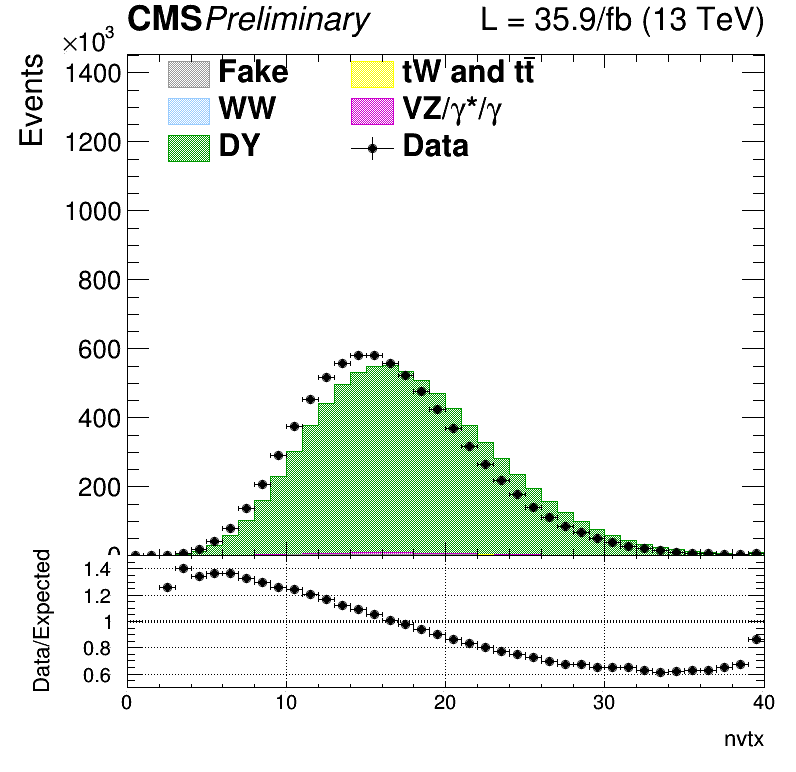
\includegraphics[width=0.45\textwidth]{Figs/nvertices.png}
\caption{
    Distributions of the number of vertices in a Drell-Yan enriched sample
    (Z$\rightarrow{}ee$) in
    data}
    \label{Fig:pu}
\end{figure*}

The pileup histogram for reweighting is calculated using the \emph{pileupCalc} tool as described in~\cite{puJSON}. 


%Cross sections
Different sources and calculations are used to obtain the cross sections for the different processes at 13\TeV. 
For Higgs signals, the cross sections used are the ones reported but the LHC Higgs Cross Section Working Group~\cite{temphiggsxsecs},
computed at NNLO and NNLL QCD and NLO EW for gluon fusion, and at NNLO QCD and NLO EW for the rest of the production modes.
The branching fractions are the ones reported in Ref.~\cite{Heinemeyer:2013tqa}. 

The cross section used for normalizing \qqbar produced WW processes was computed at next-to-next-to-leading order
(NNLO)~\cite{Gehrmann:2014fva}. The leading-order (LO) cross section for ggWW is obtained directly from \MCFM.
For gluon fusion, the difference between LO and NLO cross sections is significantly big.
A scale factor of 1.4 is theoretically calculated~\cite{Caola:2015rqy} and applied to the gg$\to$WW background. 
%The interference between the high mass resonance, the gg$\to$WW background and the H(125) has been computed using the MELA package as describe in Sec.~\ref{sec:AnalysisStrategy}.

%For the LO simulation of the interference between 
%gg$\rightarrow$WW and gluon fusion  produced H$\rightarrow$WW a k-factor of 1.87 is applied. 
%This k-factor is obtained as the average between LO to NNLO ggH scale factor and LO to NLO ggWW scale factor 
%(from private communication with the authors of~\cite{Caola:2015rqy}). 

The cross sections of the different single top processes are estimated by the LHC Top Working group~\cite{singletop} at NLO.
The \ttbar cross section is also provided by the LHC Top Working group~\cite{topxsec}, and it is computed at NNLO, with NNLL soft gluon resummation. 

Drell-Yan (DY) production of Z/$\gamma^{*}$ is generated using a\MADGRAPH~\cite{Alwall:2014hca} and the cross section is scaled using a LO to NNLO k-factor equal to 1.23. 
Other multiboson processes, such as WZ,ZZ, and VVV (V=W/Z), are generated with a\MCATNLO and normalized
to the cross section obtained at NLO in generation.
The cross sections for the remaining processes were directly obtained using the \emph{GenXSecAnalyzer}
tool~\cite{genxsec} or from the Twiki presented in Ref.~\cite{25nstwiki}.

All processes are generated using the NNPDF2.3~\cite{Ball:2013hta,Ball:2011uy} parton distribution functions (PDF) for NLO generators,
while the LO version of the same PDF is used for LO generators. All the event generators are interfaced 
to \PYTHIA 8.1 for the showering of partons and hadronization, as well as including a simulation of the 
underlying event (UE) and multiple interaction (MPI) based on the CUET8PM1 tune~\cite{Khachatryan:2015pea}.





\subsection{The DY sample}\label{sec:DY}

Given the lack of MC statistics in the LO inclusive DY sample the
$H_\mathrm{T}$-binned samples are used. This helps increasing the MC
statistics especially in the VBF category of the same flavor analysis, which is characterized by large values of $H_\mathrm{T}$.
The LO inclusive sample is used for events with $H_\mathrm{T} < 100$\GeV and it has been merged to the other samples selecting events with $H_\mathrm{T}$ below 100\GeV using the parton level information. The cross sections of those samples have been scaled applying the LO to NNLO k-factor. In Fig.~\ref{fig:DY_HT} the $H_\mathrm{T}$ distribution of the sample after the merging is reported, showing a smooth transition between different $H_\mathrm{T}$ samples.

\begin{figure}[htbp]
\centering
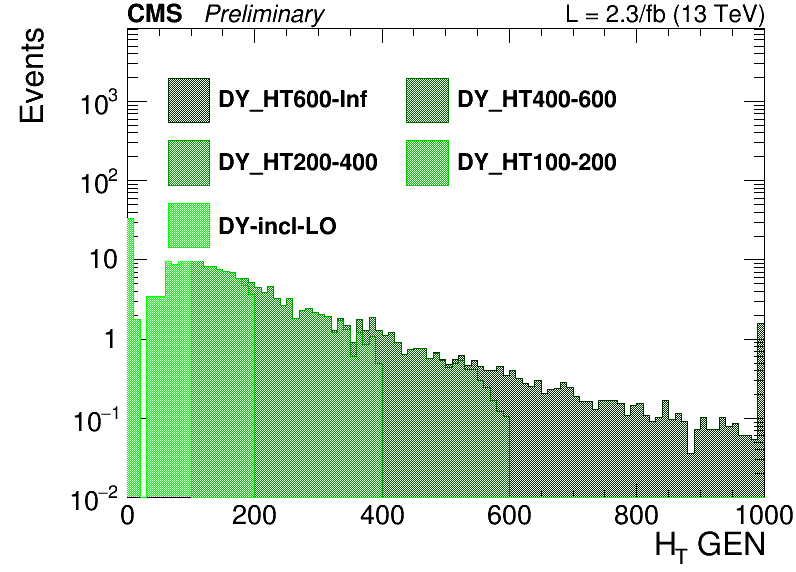
\includegraphics[width=0.6\textwidth]{Figs/log_c_incl_HTGen.png}
\caption{
    $H_\mathrm{T}$ distribution for the merged DY sample.}
    \label{fig:DY_HT}
\end{figure}


To further check the correct behaviour of the $H_\mathrm{T}$ binned samples we compared them to the inclusive LO sample, selecting only the events with a generator level $H_\mathrm{T}$ above 100\GeV. The comparison is done in a control region with two same flavor leptons with $\pt > 20$\GeV and $\mll > 50$\GeV, showing very good agreement between the two samples. The distributions of some variables are shown in Fig.~\ref{fig:inclDYvsHT}

\begin{figure}[htbp]
\centering
\subfigure[\mll]{
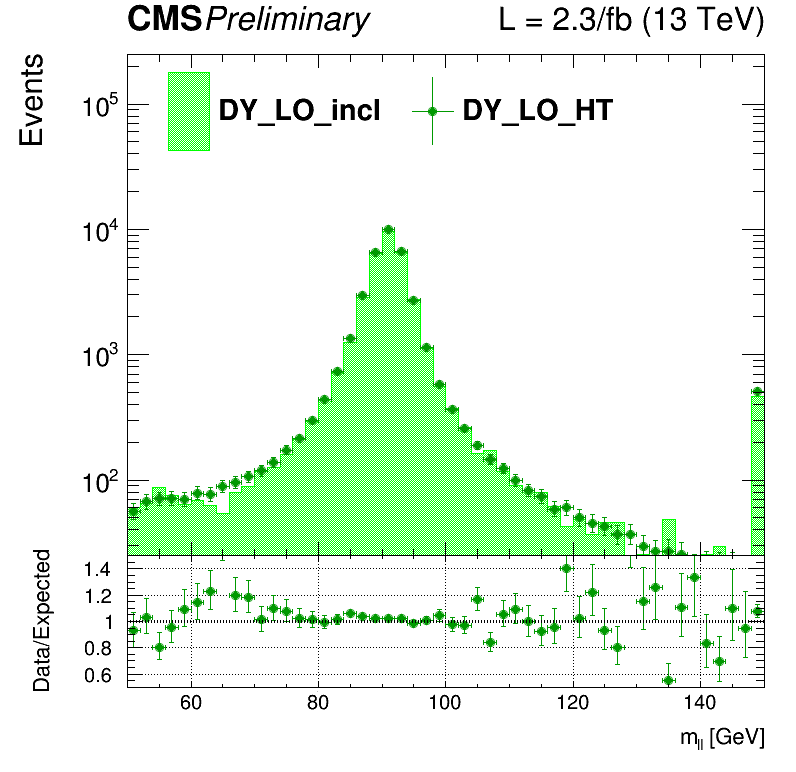
\includegraphics[width=0.45\textwidth]{Figs/DY/inclLOvsHT/log_cratio_dyee_13TeV_mll.png}
}
\subfigure[\ptll]{
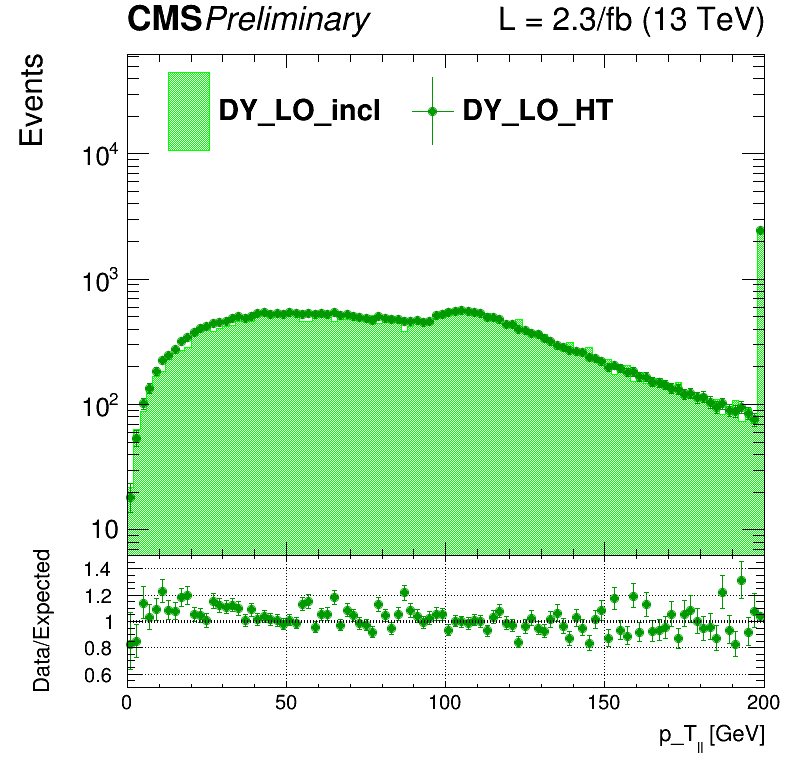
\includegraphics[width=0.45\textwidth]{Figs/DY/inclLOvsHT/log_cratio_dyee_13TeV_ptll.png}
}
\\
\subfigure[$\eta$ of leading lepton]{
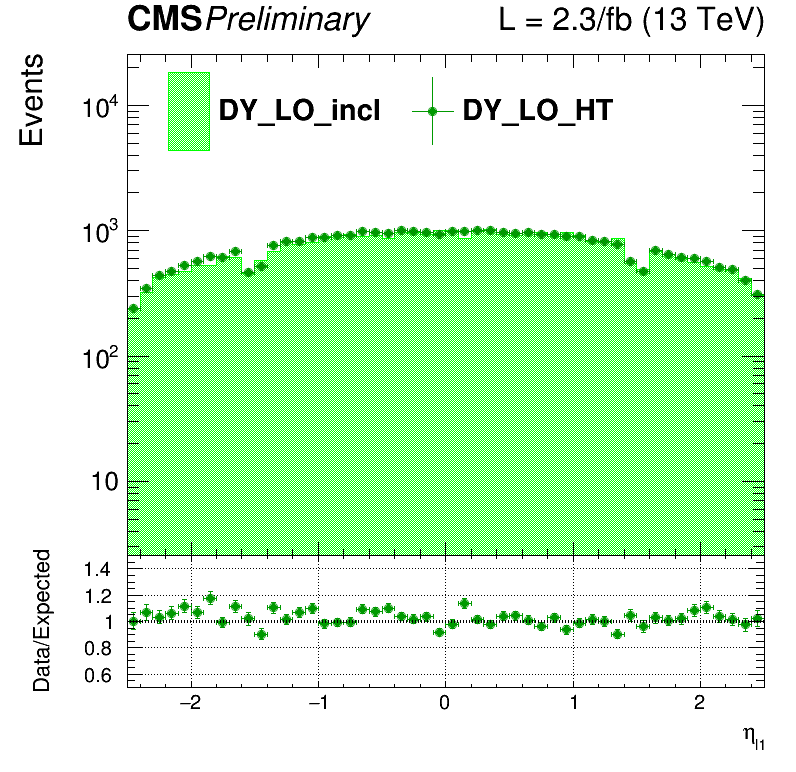
\includegraphics[width=0.45\textwidth]{Figs/DY/inclLOvsHT/log_cratio_dyee_13TeV_eta1.png}
}
\subfigure[$\eta$ of trailing lepton]{
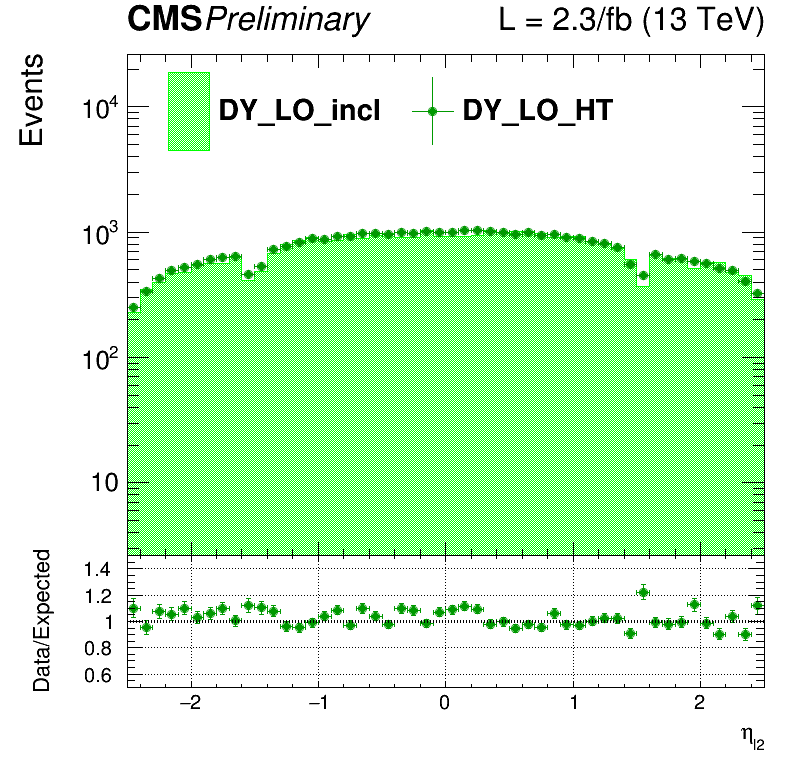
\includegraphics[width=0.45\textwidth]{Figs/DY/inclLOvsHT/log_cratio_dyee_13TeV_eta2.png}
}
\caption{
    Comparison between the inclusive LO DY sample and the $H_\mathrm{T}$ binned samples.}
    \label{fig:inclDYvsHT}
\end{figure}



To check the differences between the LO inclusive sample and the NLO sample simulated with \MCATNLO, the two samples have been compared in a same flavor control region and some variables of interest are shown in Fig.~\ref{fig:LOvsNLO}. The control region is defined requiring two same flavor leptons with $\pt > 20$\GeV and with $\mll > 50$\GeV.


\begin{figure}[htbp]
\centering
\subfigure[\mll]{
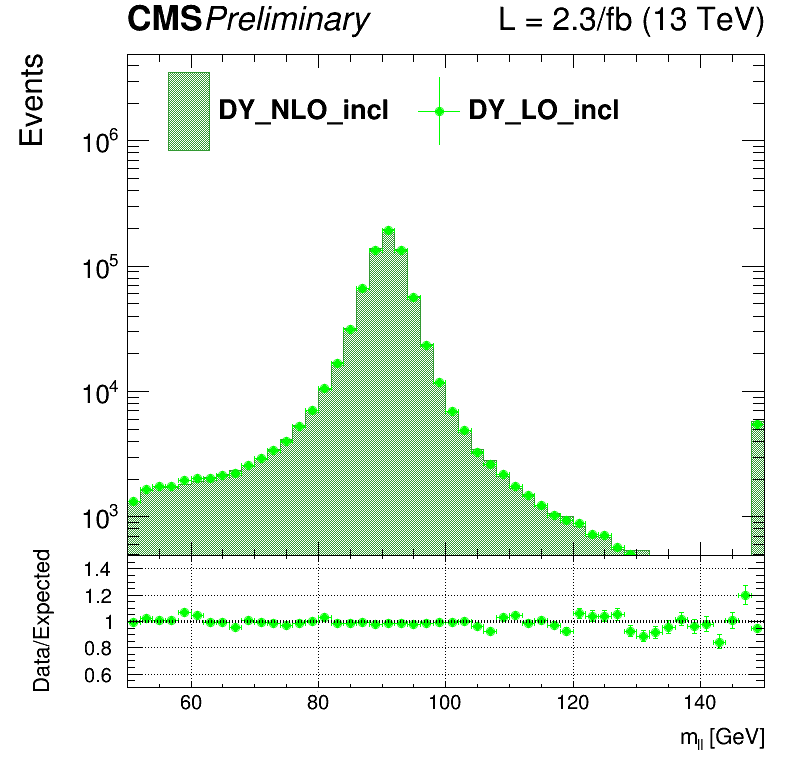
\includegraphics[width=0.45\textwidth]{Figs/DY/LOvsNLO/log_cratio_dyee_13TeV_mll.png}
}
\subfigure[\ptll]{
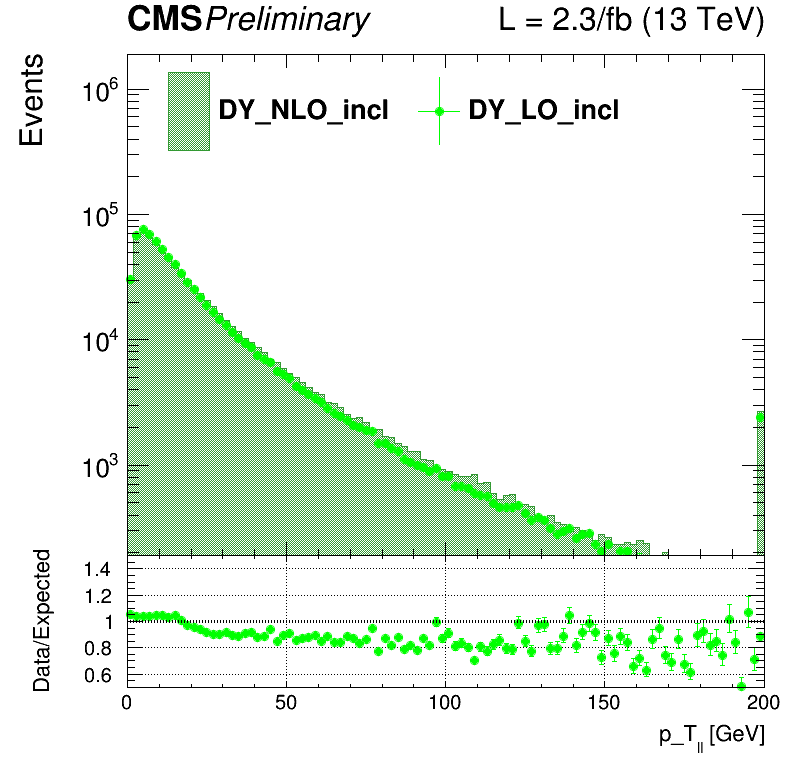
\includegraphics[width=0.45\textwidth]{Figs/DY/LOvsNLO/log_cratio_dyee_13TeV_ptll.png}
}
\\
\subfigure[$\eta$ of first lepton]{
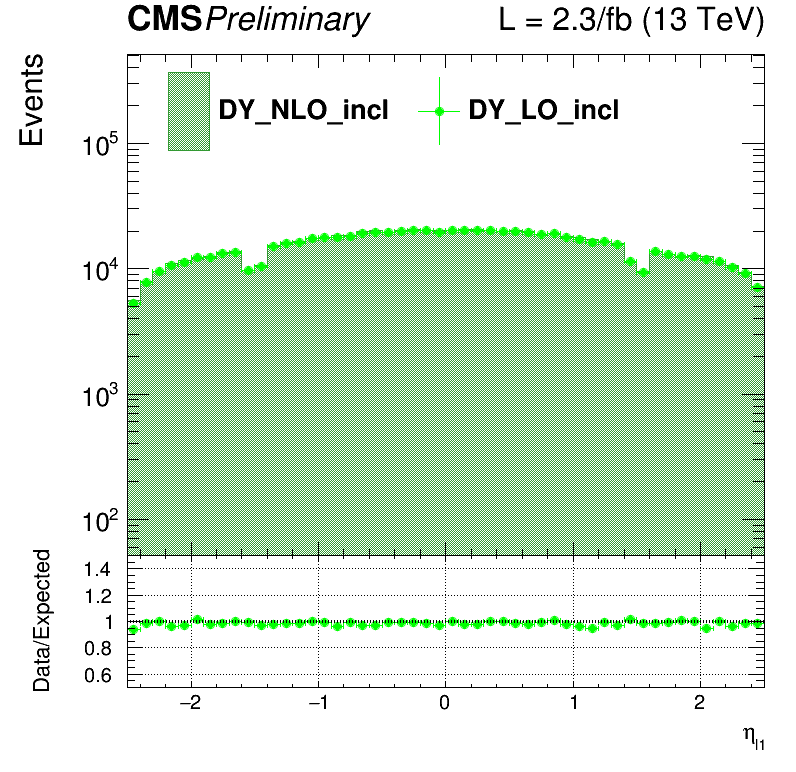
\includegraphics[width=0.45\textwidth]{Figs/DY/LOvsNLO/log_cratio_dyee_13TeV_eta1.png}
}
\subfigure[number of jets]{
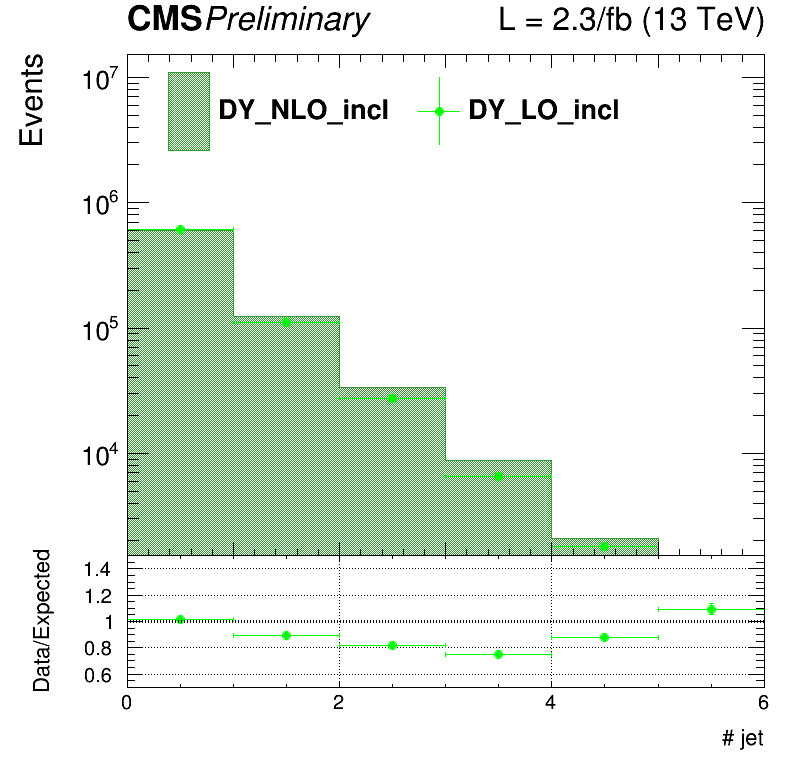
\includegraphics[width=0.45\textwidth]{Figs/DY/LOvsNLO/log_cratio_dyee_13TeV_njet.png}
}
\caption{
    Comparison between the LO and NLO DY samples.}
    \label{fig:LOvsNLO}
\end{figure}


\subsection{The WW sample}

In the analysis two different WW Monte Carlo samples are merge: the ``$WW \rightarrow 2l 2\nu$ NLO'' and the ``WW plus 2 jet'' LO (WpWmJJ-QCD-noTop in Tab. 4). 

The second sample,  ``WW plus 2 quark'', contais final state with two quarks or a gluon-quark system: only the final state with two quarks interferes with the signal.
To avoid double count between the two sample a cut on di-jet mass at gen-level,$mjj_{GenLev}$, is applied. In particular the sample ``$WW \rightarrow 2l 2\nu$ at NLO'' is used for $mjj_{GenLev} <100$ GeV and the ``WW plus 2 quark'' for $mjj_{GenLev} >100$ GeV.

The  distribution for the reco di-jet mass is shown in Fig. \ref{fig:WW}. In particular the red distribution correspond the ``$WW \rightarrow 2l 2\nu$ NLO'' sample with a cut of  $mjj_{GenLev} <100$, the blue distribution to  ``WW plus 2 quark'' with $mjj_{GenLev} >100$ GeV. The sum of the red and blue distributions is shown in black. There is a good agreement between with the black distribution and the ``$WW \rightarrow 2l 2\nu$ NLO'' without any  $mjj_{GenLev}$ distribution , in green.



\begin{figure}[htbp]
\centering
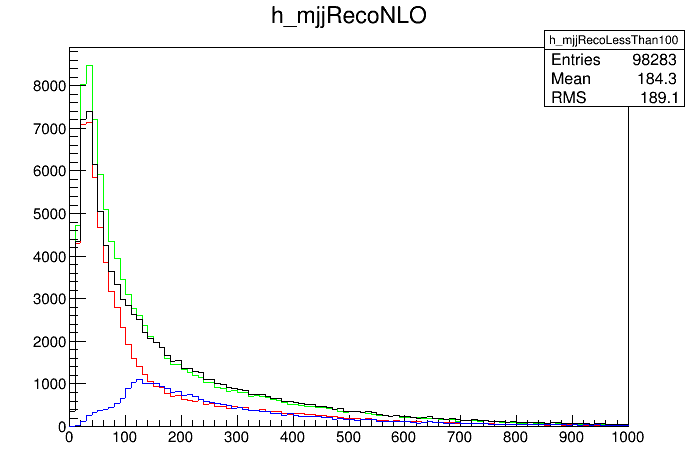
\includegraphics[width=0.6\textwidth]{Figs/WW_distribution.png}
\caption{
    Distribution for $m_{jj}$ at RECO level for the merged WW sample.}
    \label{fig:WW}
\end{figure}

 \clearpage

% ---- ---- ---- ---- ---- ---- ---- ---- ---- ---- ---- ---- ---- ---- ---- ---- ----
\section{Objects}\label{sec:Objects}

For a detailed description of the objects used in the analysis, including the
trigger strategy and fake rates estimation, refer to AN-2017/082.
 \clearpage

% ---- ---- ---- ---- ---- ---- ---- ---- ---- ---- ---- ---- ---- ---- ---- ---- ----

\textit{%As described in Sec.~\ref{NSP}, the research of  new resonance $X$ is one of the mail goals of LHC. With a energy achieved of 13 TeV in the center of mass and the data collected in 2016, it is possible to lead searches in a vast range of mass. One of the main final state channel in in a couple of $W^+W^-$ bosons.
In this chapter the $X \to \mathrm{W^+W^-}\to2\ell2\nu$ analysis using 2016 data is reported. To increase the sensitivity of this search, the signal must be selected in the most efficient way by reducing the
presence of the backgrounds with a similar signature: the selection criteria are described in detail. I have participated at all stages of the analysis selection (signal simulation, categorization, background estimation, etc.)  and I have been responsible for the whole analysis.} 
%The ATLAS experiment has been done this kind of searches using the early 2016 statistic, 13.2 fb$^{-1}$ and the results are shown in Fig.~\ref{ATLAS-CONF-2016-074_fig}.
%With the full 2016 statistic, approximately $\sim 36$ fb$^{-1}$ is possible to investigate a wide range of masses and, if will be no evidence of high mass signal, is possible to set  tight upper limits on the possible cross section.

\section{Overview of the fully leptonic analysis }\label{sec:AnalysisStrategy_Intro}
The analysis strategy for the high mass search in the $X \to \mathrm{W^+W^-}\to2\ell2\nu$ final state must take into account the production modes of the new scalar, the main backgrounds, and the interference among the different processes. 

The main production mode for a Higgs-like particle over the all mass spectrum is the gluon-gluon fusion process. 
However the ratio of the VBF cross-section to the gluon-gluon fusion cross-section increases with $m_\mathrm{X}$ (see Fig.~\ref{prod}), making the VBF production mechanism more and more important.\\

Among the SM processes that have the same final state of the signal or a similar one the most important are non-resonant WW production, top production, Drell-Yan. The WW production is an irreducible background and needs to be determined together with the signal in the fit. To estimate the other background processes, control regions are defined on data and compared to simulation. \\
The events are first divided according the flavour in the final state: 
\begin{itemize}
\item opposite-flavour final state, $e^{\pm} \mu^{\mp}$,
\item same-flavour final state, $e^+ e^-$ and  $\mu^+ \mu^-$. 
\end{itemize}
In the opposite-flavour final state four different jets categories are defined: the 0-jet, the 1-jet, the 2-jet and the VBF, Sec.~\ref{sec:OF}. 
In the same-flavour final state only the VBF category is considered. Indeed, only the VBF selection cuts are sufficiently tight to reduce the  overwhelming Z plus jets background to a manageable level, Sec.~\ref{sec:SF}. The jets categories improve the sensitivity of the analysis, because each category has different contributions from signal production modes and backgrounds.

The signal is interpreted in terms of the EWK singlet and MSSM models as described in Sec~\ref{NSP}. The Higgs boson width and lineshape is reweighted at generator level according to the parameters defined in the model. The interference effects between the signal produced via gluon-gluon fusion, the WW background also from gluon-gluon fusion, and SM Higgs boson, are expected to change the shape of the signal distribution and have been fully taken into account. 
A similar treatment is also applied for the interference between high mass signal produced via VBF, the WW plus two quarks background (emerging from the same initial state) and the SM Higgs generated with VBF production mechanism. In general, the interference becomes more and more important as the mass of $X$ increase and it is studied in detail in Sec~\ref{sec:signalModel}.
Finally, the interference between the $\mathrm{W^+W^-}\to2\ell2\nu$ and $\mathrm{ZZ}\to2\ell2\nu$ is negligible due to the different phase space characteristic of these processes.




\section{Main Background processes}
\label{anbkg}
Inside the SM that are several processes that have the same or a similar final state of the signal. The most important background processes contributing to this final state are non resonant $q\bar{q} \to W^+ W^-$, the top production ($t\bar{t}$ and single-top) and the Drell-Yan process. 
Other backgrounds are due to $W$+jets events, where a jet is misidentified as a lepton, and multibosons events. 
All these processes have been simulated with Monte Carlo generators and the simulation details have been discussed in Sec~\ref{MSsample}.
A detailed description of these background processes is given below:
\begin{itemize}
\item \textit{Non-resonant WW} ($q\bar{q} \to W^+ W^-$): this background is characterized by a final state identical to the signal, however the lepton kinematics for signal and $q\bar{q} \to W^+ W^-$ processes is rather different.
For the signal process, the W bosons originate from a spin-0 particle decay
and their spins must therefore be antiparallel, implying that the charged leptons produced 
in their decays appear preferentially in the same hemisphere~\cite{Ellis:2012wg}. In contrast,
there is no preferential spin direction in the background case. For this reason the
azimuthal angle difference between the two leptons is on average smaller for signal
than for background, resulting in a smaller dilepton invariant mass in the former case. The most relevant Feynman diagram of the process is shown below.
\begin{figure}[h]
\centering
\vspace{0.5cm}
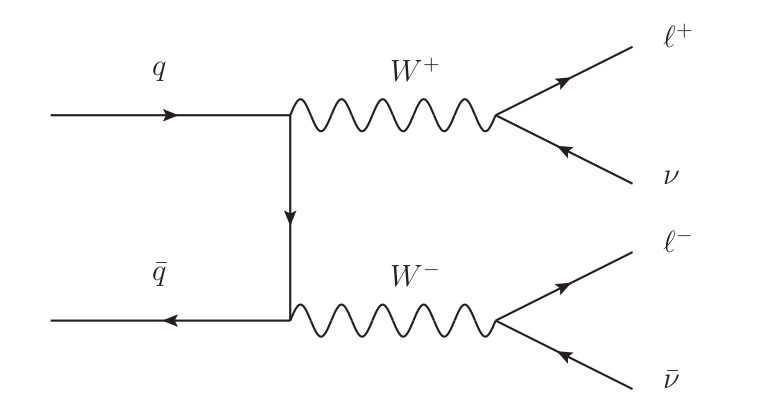
\includegraphics[scale= 0.9]{../Cap5/nnr_WW}
\end{figure}
\item \textit{Top} ($t\bar{t}$ and single-top): the $t\bar{t}$ events give a signal-like signature if both decays $t \to Wb$ are followed by $W \to \ell \nu$.  In such a case, in fact, there are two leptons and missing transverse energy,  plus two jets (from the hadronization of the $b$ quark) in the final state. This process is especially important when the signal is produced via VBS or when the signal is associated with jets coming from initial or final state radiation. The single-top production is characterized by the presence of a $W$ boson and a top quark, so after the top decay, again by two W's, but only one b-jet. Following, some examples of Feynman diagrams for the top background: the $t\bar{t}$ in (a) and (b) diagrams, the single-top in (c).
\begin{figure}[h]
\centering%
\subfigure[]%
{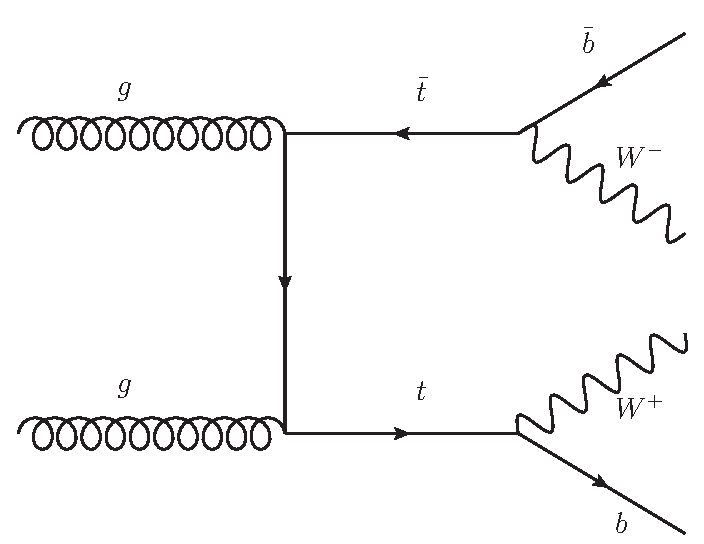
\includegraphics[scale= 0.3]{../Cap5/ggtt_t}} \qquad 
\subfigure[]%
{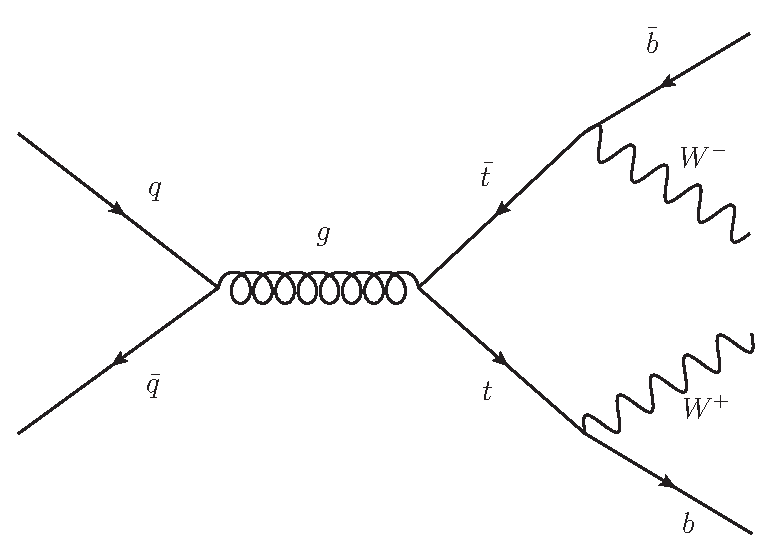
\includegraphics[scale= 0.3]{../Cap5/qqtt_s}} \qquad 
\subfigure[]%
{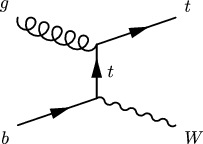
\includegraphics[scale= 0.5]{../Cap5/st_bg}}
\end{figure}
%\newpage
\item \textit{Drell-Yan}: the Drell-Yan process is defined as the annihilation of a quark-antiquark pair into a lepton-antilepton pair. This process is described at leading order by
the two  shown Feynman diagrams. %These amplitudes are proportional to the fine structure constant $\alpha \sim 1/137$.
This kind of background is particularly important for the same flavour final state of the signal
\begin{figure}[h]
\centering
\vspace{0.5cm}
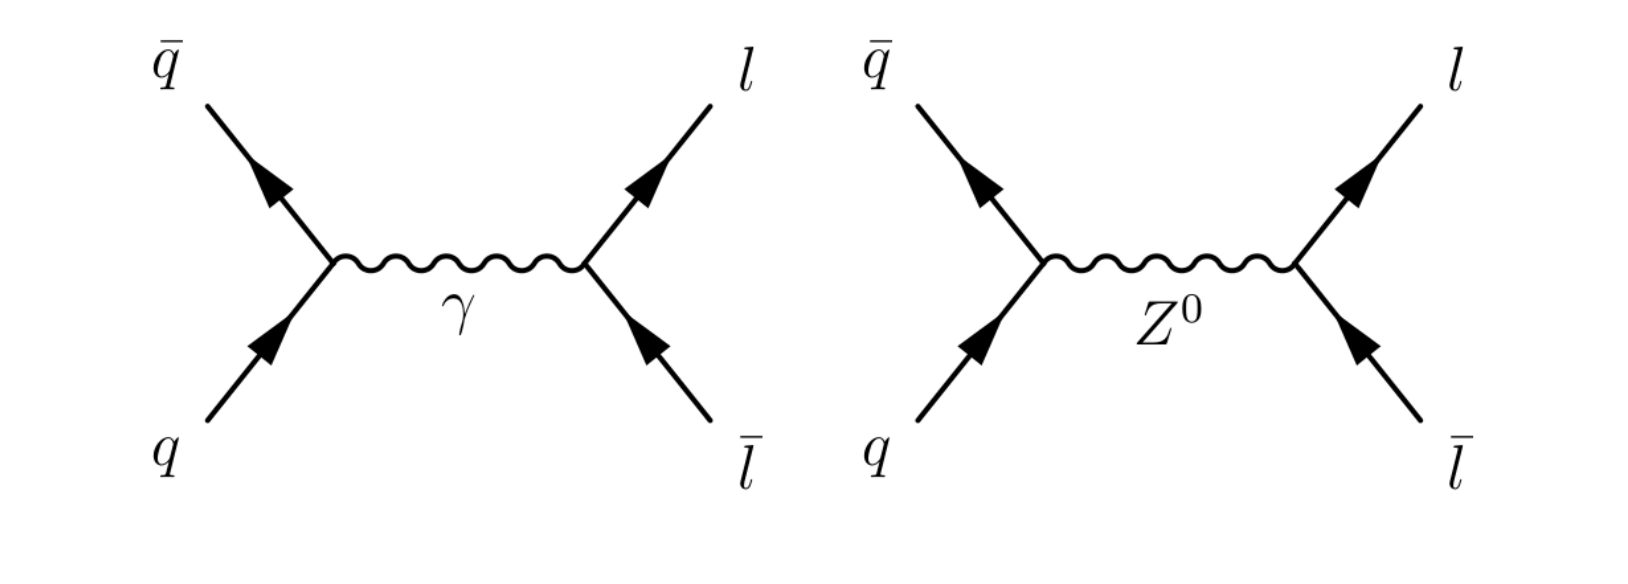
\includegraphics[scale= 0.7]{../Cap5/dy}
\end{figure}

\item \textit{W+jet}: this background is charaterized by a $W$ boson, decaying in $\ell \nu$, produced in association with a jet. If a fake lepton arise from the misidentified jet, these events have  the same final state of the signal (two leptons and missing-transverse-energy), Sec~\ref{fk}. 

\item \textit{Other}: other background processes involve multibosons production, such as $WZ/W\gamma^*$, $ZZ^*$ and $Z\gamma$ with $\gamma$ conversion.

\end{itemize}
The main background processes, the \WW production and the top production, are estimated using data. 
Instrumental backgrounds arising from non-prompt leptons in $W+$jets production and mis-measurement of $E_T^{miss}$ in Drell-Yan events are also estimated from
data. The contribution from W$\gamma^*$  is estimated partly from data. The
contribution of other sub-dominant backgrounds is obtained directly from simulated samples. The different data-driven background estimations are explained in the following sections. 
%More precisely top and  Drell-Yan backgrounds normalizations have been extracted
%directly from data-simulation comparison in specific control regions enriched in either one
%or the other background separately for the different events categories, using the rateParam feature of the combine package~\cite{combine}.


\section{Fake Lepton Background Estimation}
\label{fk}
Lepton fake rates are measured as a
function of the lepton $p_T$ and $\eta$, in a single lepton triggered sample. The test of the method and
systematic errors are described below.
In the analysis
the primary source of background from misidentification is W+Jets. QCD multi-jet and hadronic top backgrounds
are also present at much smaller level. Events in which W bosons are produced in association
with jets give rise to background to WW events when a jet is misidentified as a lepton. These
events contain a real lepton and real missing energy from the W decay. With the jet misidentified 
as a lepton, the W+Jets events have two identified leptons, missing energy, and no other
significant event characteristics. As a result, the W+Jets events cannot be easily suppressed
by event selection. This background is particularly important at low $p_T$.
The estimation of the fake lepton contribution is based on the ``fakeable object'' data-driven
method and provides a measurement of the yield and the kinematic distributions of fake background. 
It is a general technique, applicable to any physics analysis in which particle level
selection criteria are used to suppress background. The method can be used with any number
of final state particles and is independent of the event selection.
The fundamental idea of the fakeable objet method is simple: select a control sample of events
enriched in the background being estimated, and then use an extrapolation factor to relate these
events to the background in the signal region. The method is data-driven provided the control
sample is selected in data, and the extrapolation factor is measured with data. For background
arising from particle misidentification, the extrapolation is done in particle identification space
($p_T$ and $\eta$ ) of the lepton. The control sample is defined using a looser particle selection criteria
that are chosen such that the rate of misidentification is increased. The extrapolation factor
relates background misidentified with this criteria, to background misidentified as passing the
full particle selection of the signal region.



\section{Lepton Efficiencies from Tag and Probe Method}
\label{TP}
One of the well established data-driven approach for measuring the particle efficiencies is the
so called Tag and Probe method. The Tag and Probe method uses a known mass resonance (e.g. $J/\Psi$, $Z$) to select particles of the desired type, and probe the efficiency of a particular
selection criterion on these particles. In general the “tag” is an object that passes a set of very
tight selection criteria designed to isolate the required particle type. Tags are often referred
to as a “golden” electrons or muons and the fake rate for passing tag selection criteria should
be very small. A generic set of the desired particle type (i.e. with potentially very loose selection 
criteria) known as “probes” is selected by pairing these objects with tags such that the
invariant mass of the combination is consistent with the mass of the resonance. Combinatoric
backgrounds may be eliminated through any of a variety of background subtraction methods
such as fitting, or sideband subtraction. The definition of the probe objects depend on the specifics of the selection criterion being examined. The simple expression to get the efficiency %as a function of $p_T$ and $\eta$ 
is given below:
\begin{equation}
\epsilon=\frac{N_{Pass}^{Probes}}{N_{Pass}^{Probes}+N_{Fail}^{Probes}}
\end{equation}

\subsection*{Electrons} 
The   Tag and Probe is used here to get the identification and isolation efficiency of electrons. In this case, the Tag is a
well identified and isolated electron which also passes an electron trigger. 
Once the Tag electron is selected then another object that pass the kinematic electron selection, Tab.~\ref{IDe}, is searched for. 
The invariant  mass of the Tag and the Probe electron pair is reconstructed and must be in window around the Z boson mass. 
After that, to compute the efficiency, the Probe electron is required  to pass the identification tight working point. 
This procedure is performed for the data and the MC samples. 
Once data and MC efficiencies have been calculated, the electron scale factors are estimated as the ratio among the data and MC efficiencies.  
These scale factors are calculated as a function of $p_T$ and $\eta$ and used to correct the difference in efficiencies between data and MC in the analysis. 
%The Pile-Up reweighting is also applied on MC during the computation of efficiencies. 
%A MC truth matching has also been applied in case of the computation using simulation. 
%In principle, there are two methods to estimate the efficiencies.
%The first one is the \textit{counting method} and the other one is the \textit{fitting method}. 
%The counting method is used when there  are small backgrounds, instead  the fitting method instead when the backgrounds are 
%In order to take into account the effect of DY background in the efficiency estimation,  a fitting method has been used. 
%Tag and Probe pairs are  selected in Z mass window of 60 to 120 GeV.
%If there exist more than one pair then the one whose invariant mass closer to Z pole mass has been selected.
%The efficiencies have been computed as a function of $p_T$ and $\eta$ of electron.
%For signal fitting, MC templates are derived from the simulated sample in the Z mass range 60 to 120 GeV in  $p_T$ and $\eta$ bins.
%The MC Templates are then smeared using Gaussian function. For the background fitting a function, that is combination of
%an exponential function and an error function, has been used.
%The exponential decay distribution becomes
%active at high mass beyond the Z peak and the error function takes over at low masses due to
%threshold effect.
%A fit examples for all $p_T$ bins is shown in Fig.~\ref{ac}
%\begin{figure}
%\centering
%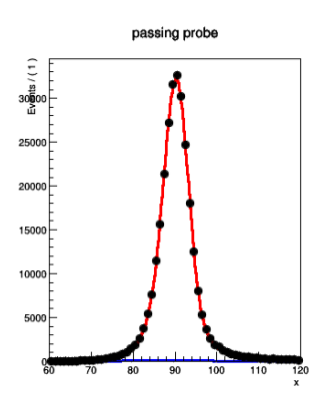
\includegraphics[scale= 0.5]{tpe}
%\caption{Fits for $p_T$ bin (35-50) GeV and $\eta$ in (-2.5,-2.0) bin.}
%\label{ac}
%\end{figure}

The electron efficiency is about 95\%, on the trigger plateau. 


\subsection*{Muons} 
The muon identification and isolation efficiency is also studied and compared to the prediction of MC in order
to understand if a correction is needed. The muon efficiency is obtained as
\begin{equation}
\epsilon_{\mu} = \epsilon_{TRK} \times \epsilon_{Tight} \times \epsilon_{ISO \; Tight} \; ,
\end{equation}
\newline
where $ \epsilon_{TRK}$ is the tracker  muon efficiency.  
The $ \epsilon_{Tight} $ is muon efficiency
under the assumption that the muon passes the kinematic selections summarized in  Tab.~\ref{IDm}.
The $\epsilon_{ISO \; Tight}$ is the efficiency of the isolation criteria under the assumption that the muon passes the same selection.
The $\epsilon_{Tight}$ and $ \epsilon_{ISO \; Tight}$ are determined  using the Tag and Probe method. 
The Tag muon is obtained by applying  the kinematic selections  and   the isolated muon trigger  with $p_T^{\mu}>20$ GeV.
The Probe muon  is requested to pass the kinematic selection and the isolation criteria.
%After that it is checked if the Probe muon is matched to the muon trigger. 
%In general the efficiencies are relatively high due to the lower cut on $p_T$ and the looser cut on
%isolation %in the double lepton trigger compared to single muon trigger. 
The efficiency value on the plateau is around 93\%-99\%.



\section{Data sample and Trigger used}

%\subsection*{Data sample}
%\subsection*{Data in CMS}
Data recorded in proton proton collisions at 13 TeV during all 2016 was used in the analysis, with a total integrated luminosity of  35.9 \fbinv.
%The data has been reprocessed in the reprocessing campaign characterized by the submission date \textit{03Feb2017} in CMS.
%In Table~\ref{tab:data} the different data streams used are presented. 
All runs are taken with a 25~ns LHC filling scheme and recorded in seven different periods, namely Run2016C, Run2016D, Run2016E, Run2016F, Run2016G, and Run2016H.
% \begin{table}
% \begin{center}
% \begin{tabular}{|l|l|}
% \hline
% Data Taking Era & Stream\\
% \hline
% \multirow{5}{*}{Run2016C} 	& SingleMuon  \\
%                                 & DoubleMuon \\
% 				& SingleElectron \\
%                                 & DoubleEG \\
% 				& MuonEG \\ \hline
% \multirow{5}{*}{Run2016D}       & SingleMuon  \\
%                                 & DoubleMuon \\
%                                 & SingleElectron \\
%                                 & DoubleEG \\
%                                 & MuonEG \\ \hline
% \multirow{5}{*}{Run2016E}       & SingleMuon  \\
%                                 & DoubleMuon \\
%                                 & SingleElectron \\
%                                 & DoubleEG \\
%                                 & MuonEG \\ \hline
% \multirow{5}{*}{Run2016F}       & SingleMuon  \\
%                                 & DoubleMuon \\
%                                 & SingleElectron \\
%                                 & DoubleEG \\
%                                 & MuonEG \\ \hline
% \multirow{5}{*}{Run2016G}       & SingleMuon  \\
%                                 & DoubleMuon \\
%                                 & SingleElectron \\
%                                 & DoubleEG \\
%                                 & MuonEG \\ \hline
% \multirow{5}{*}{Run2016H}       & SingleMuon  \\
%                                 & DoubleMuon \\
%                                 & SingleElectron \\
%                                 & DoubleEG \\
%                                 & MuonEG \\ \hline
% \hline 
% \end{tabular}
% %\vspace{0.5cm}
% \caption{Data samples used in the analysis. The total integrated luminosity corresponds to 35.9\fbinv.
% \label{tab:data}}
% \end{center}
% \end{table}


%\subsection*{Triggers path and  efficiency}
Events are required to fire one of the unprescaled single-electron, single-muon or
muon-electron triggers. Due to the rather high LHC instantaneous luminosity the
single-lepton triggers must have high HLT $p_T$ thresholds, otherwise the rate of these
triggers would be too large to be sustained. The double-lepton triggers allow the $p_T$
thresholds to be lowered while keeping a sustainable trigger rate.
%, thus maintaining a
%good sensitivity to the Higgs boson signal, for which the lepton  $p_T$ can be rather small.
The triggers used in this analysis are summarized in Table~\ref{tab:triggers}. 
%Since a final state with two leptons is searched for, both single and double lepton triggers are used. 
%For the electrons a combination of triggers is necessary to increase the statistics and to adjust the $p_T$ threshold requirement. 
\begin{table}
\begin{center}
\begin{tabular}{|l|l|}
   \hline
   Trigger name & HLT Threshold \\
   \hline
   
   SingleElectron & $p_T>$ 27 GeV  \\

   \hline
        
   SingleMuon   &  $p_T>$ 22 GeV  \\

   \hline
   
   MuonElectron       &  $p_T>$ 17 GeV  and 8 GeV  \\
   
   \hline
   
   DoubleMuon   & $p_T>$ 17 GeV  and 8 GeV  \\
      
   \hline
   
   DoubleElectron   &  $p_T>$ 23 GeV  and 12 GeV    \\
   
   \hline
\end{tabular}
\caption{Transverse momentum thresholds applied in the lepton triggers at the HLT
level. Double set of thresholds indicates the thresholds for each leg of the double lepton
triggers.}
\label{tab:triggers}  
\end{center}
\end{table}\\
\newline
The trigger efficiencies are calculated for leptons that pass the identification and isolation criteria.
In Fig.~\ref{Fig:trigger} the trigger efficiency for a gluon-gluon fusion signal with mass 300~\GeV is shown for electrons (left) and muons (right).
An average trigger efficiency greater than 99\% is found, as shown in Figure~\ref{Fig:triggerIntegral}. The triggers used in the analysis are summarized in Table~\ref{tab:triggers}. 
\begin{figure*}[htbp]
\centering
\begin{tabular}{cc}
%  \includegraphics[width=0.45\textwidth]{Figs/Trigger/ele.png} &
%  \includegraphics[width=0.45\textwidth]{Figs/Trigger/mu.png} \\
%  (a) electron & (b) muon \\
 \includegraphics[width=0.45\textwidth]{../AN/Figs/Trigger/ele1.png} &
 \includegraphics[width=0.45\textwidth]{../AN/Figs/Trigger/mu1.png} \\
 (a) electron 1st & (b) muon 1st \\
 \includegraphics[width=0.45\textwidth]{../AN/Figs/Trigger/ele2.png} &
 \includegraphics[width=0.45\textwidth]{../AN/Figs/Trigger/mu2.png} \\
 (c) electron 2nd & (d) muon 2nd \\
\end{tabular}
\caption{
      Trigger efficiency per event
      as a function of the lepton \pt
      for electrons (a) where leading lepton is an electron, 
      and (c) where trailing lepton is an electron, 
      and muons (b) where leading lepton is a muon, 
      and (d) where trailing lepton is an muon, 
      for a gluon fusion 300~\GeV MC sample.
      In this plots the other lepton not shown is
      integrated.
      An average trigger efficiency greater than 99\% is found.      
     }
    \label{Fig:trigger}
\end{figure*}
\begin{figure*}[htbp]
\centering
 \includegraphics[width=0.6\textwidth]{../AN/Figs/Trigger/triggW.png}
\caption{
      Trigger efficiency distribution for 
      four MC samples corresponding to masses of 300, 500, 1000 and 3000~\GeV.
      An average trigger efficiency greater than 99\% is found.
     }
    \label{Fig:triggerIntegral}
\end{figure*}



\section{Discriminating variable}
This analysis is a shape analysis, meaning that after applying selection cuts, the events are not simply counted, but rather an histogram of a discriminating variable is filled from the data and fitted with the sum of signal and background templates, and finally the signal yield is extracted.
In principle, the variable with the best discriminating power would be the invariant mass of
the four lepton system, however, due to the presence of the neutrinos, it can not be measured.
Usually, in the the Higgs boson to $WW \to 2\ell 2\nu $, the variables used in the analysis are:
\begin{itemize}
\item the transverse mass, $m_T^H$, defined as,  
\begin{equation}
 m_T^H = \sqrt{2p_{\rm T}^{\ell\ell}\MET(1-\mathrm{cos}\Delta\phi(\ell\ell, \ptvecmiss))}
\end{equation}
where $\Delta\phi(\ell\ell, \ptvecmiss)$ is the azimuthal angle between the dilepton momentum and \ptvecmiss;
\item the di-lepton mass, $m_{\ell \ell}$.
\end{itemize}
However, both $m_T^H$ and $m_{\ell \ell}$, are not sensitive to different
signal mass hypothesis. For this reason a new variable, the visible transverse mass,  $m_T^I$, has been used.
This variable, studied for this specific analysis, is defined as the invariant mass of the four momentum resulting from the sum of the
two leptons four-momenta and the missing four-momentum: 
\begin{equation}
 m_T^I = \sqrt{ (p_\mathrm{\ell\ell} + \MET)^2 - (\vec{p}_\mathrm{\ell\ell} + \ptvecmiss)^2 \; .}
\end{equation}
The distribution of all the variables defined above can be compared in 
Fig.~\ref{fig:mt_nocuts}, where it is visible the better power of $m_T^I$ in discriminating different mass hypotheses wth respect to  $m_T^H$ and $m_{\ell \ell}$. The usage of  $m_T^I$ also provides a good discriminating power between signal and background.
The effects of the interference (Sec~\ref{sec:interference}) for the discriminating variable  $m_T^I$  used in the analysis is shown in Fig~\ref{nocut_mti_700_sign}
The interference is not negligible and it will take in account as part of the signal during the fit.
\begin{figure}[htbp]
\centering
\subfigure[True generated mass]{
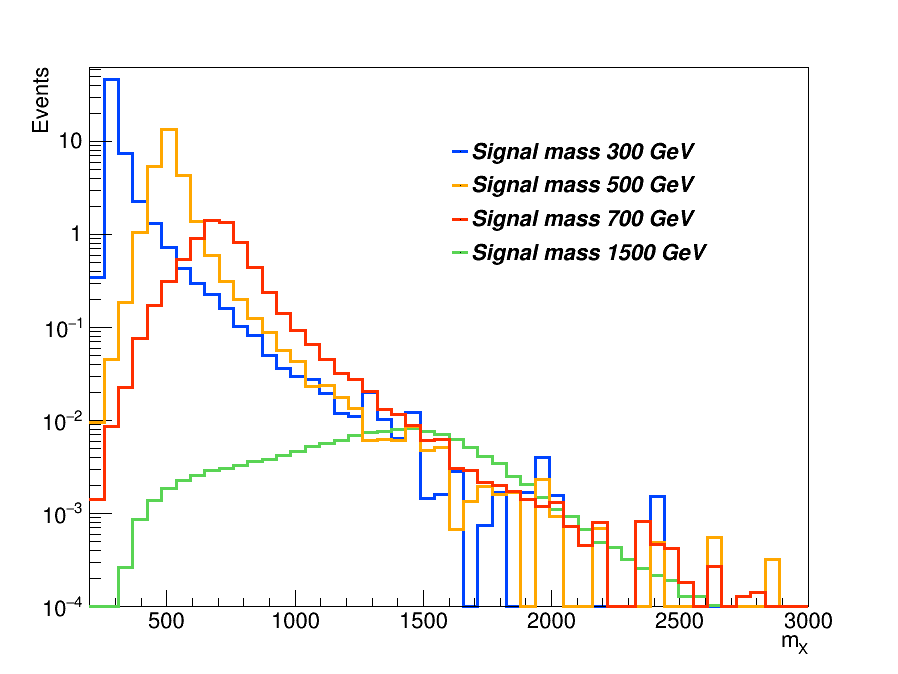
\includegraphics[width=0.45\textwidth]{../AN/Figs/Distribution_higgsLHEmass_cuts_nocuts.png}
}
\subfigure[$m_T^H$]{
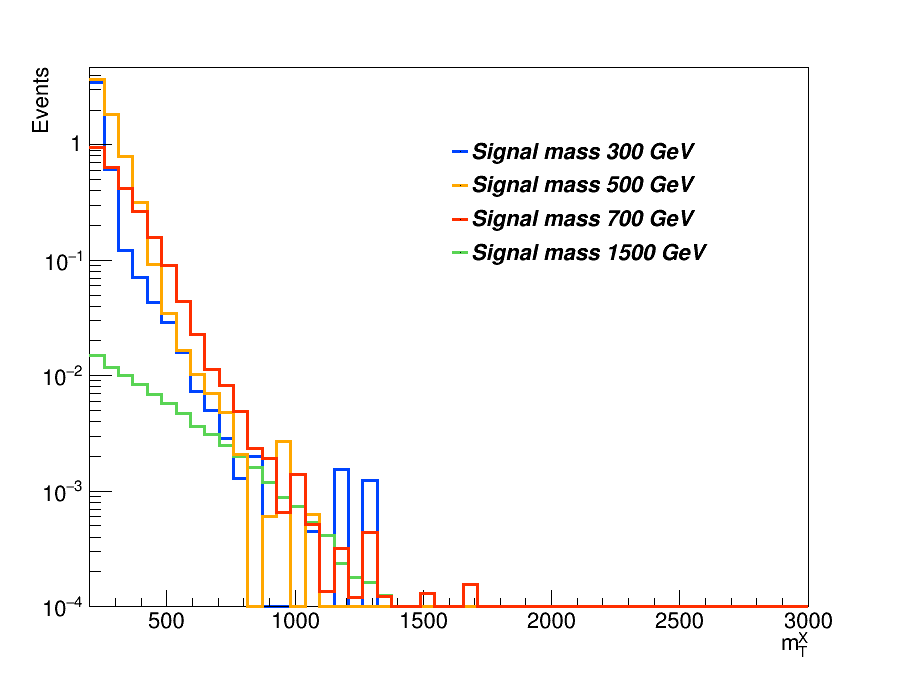
\includegraphics[width=0.45\textwidth]{../AN/Figs/Distribution_mth_cuts_nocuts.png}
}
\\
\subfigure[$m_{\ell \ell}$]{
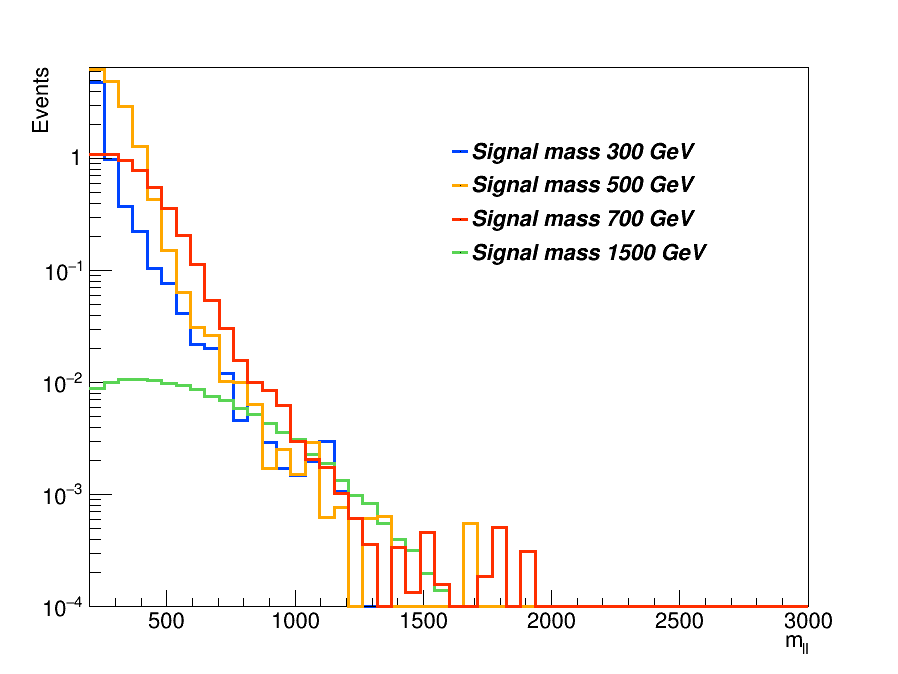
\includegraphics[width=0.45\textwidth]{../AN/Figs/Distribution_mll_cuts_nocuts.png}
}
\subfigure[$m_T^I$]{
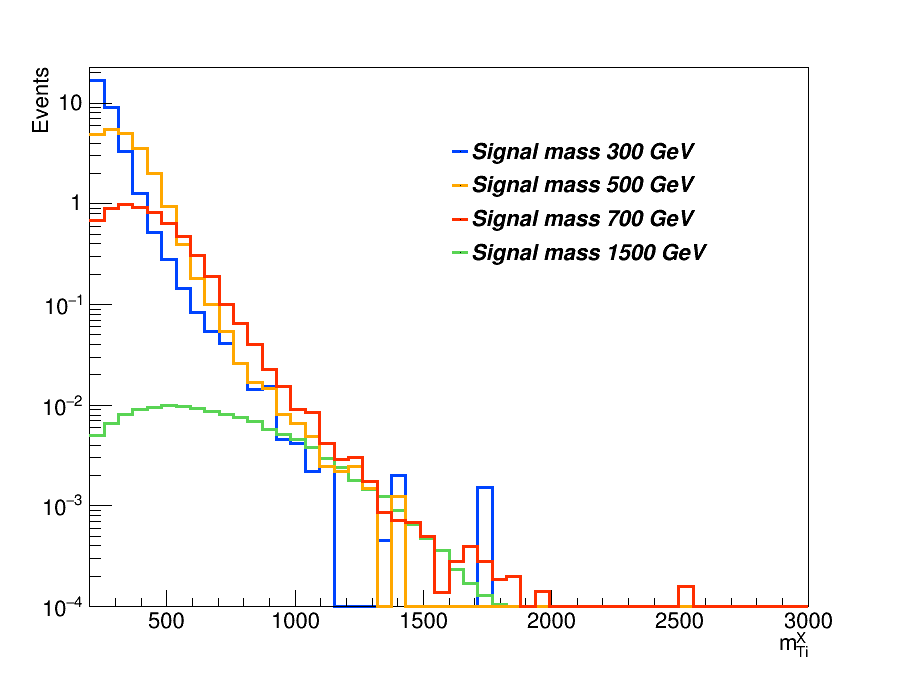
\includegraphics[width=0.45\textwidth]{../AN/Figs/Distribution_mTi_cuts_nocuts.png}
}
\caption{
    Distributions of the generated mass (no possible reconstruction), $m_T^H$, $m_{\ell \ell}$ and  $m_T^I$
    variables for different $X$ mass hypothesis. It is clear that the most discriminating variable is $m_T^I$. }
    \label{fig:mt_nocuts}
\end{figure}

\begin{figure*}[htbp]
\centering
 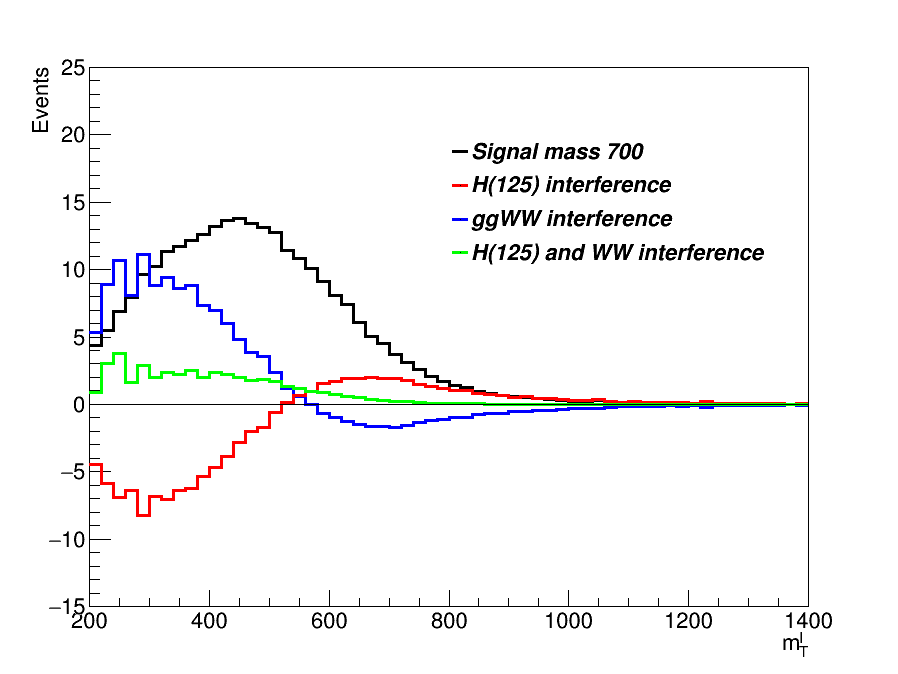
\includegraphics[width=0.6\textwidth]{../Cap5/nocut_mti_700_sign}
\caption{ The $m_T^I$ distribution at generator level for a $X$ resonances at 700 GeV produced via gluon-gluon fusion. In red the interference between the high
mass signal and the Higgs boson. In blue the interference between the high mass signal
and the background. In green the total interference i.e. high mass signal, Higgs bison and
background.       }
    \label{nocut_mti_700_sign}
\end{figure*}
 \clearpage

% ---- ---- ---- ---- ---- ---- ---- ---- ---- ---- ---- ---- ---- ---- ---- ---- ----
\newpage
\section{Opposite Flavor final state}\label{sec:OF}
\subsection*{General overview}

The events are subdivided in signal and control regions. The signal events are expected to fill  mainly to first one. Instead the second one are expected to be fill 
up by backgrounds events and they are used to normalized the backgrounds shape.\\
\newline
To avoid a possible bias of the experimenter in the process of developing the analysis
strategy and optimizing the selection requirements, firstly a blind analysis has been performed
by defining a background-only sideband control region and only looking at data events
falling in such a region. Precisely, the control region is defined according to  selection
criteria that exclude the signal events. 
Data in the signal region, i.e.  were not examined until the event selection
criteria were settled, only relying on Monte Carlo simulations for what concerns signal. 
In this way, the analysis strategy has been decided looking at the simulated events. 
Only when data distributions in signal-depleted regions confirmed the robustness of the analysis, data in
signal region were inspected. For these reasons, the agreement between data and Monte Carlo was
checked on a sideband region.




\subsection*{Signal region}
The events are requested to pass single or double lepton triggers, and exactly one electron and
one muon are requested to be reconstructed in the event. 
One of the two leptons is requested to have a $p_T$ greater than 25 GeV , the other is
requested to have  $p_T$ greater than 20 GeV and both leptons are requested to be well identified
and isolated, to reject non-prompt leptons and leptons coming from QCD sources. To suppress
background processes with three or more leptons in the final state, such as ZZ, WZ, Z$\gamma$, W$\gamma$
or triboson production, no additional identified and isolated lepton with $p_T >$  10 GeV should
be reconstructed. The low dilepton invariant mass region dominated by QCD production of
leptons is not considered in the analysis and $m_{\ell \ell}$  is requested to
be higher than 50 GeV to reduce the SM Higgs boson ($m_H$=125 GeV)
contamination. A moderate cut on the missing-transverse-energy is applied (MET $>$ 20 GeV) due to the
presence of neutrinos in the final state. Since a high mass
signal is searched a cut on $m_T^I >$ 100 GeV is applied.
A cut on the transverse momentum ($p_T^{\ell \ell} >$30 GeV) and on the $m_T^H
>$ 60 GeV are applied against $DY\rightarrow{}\tau\tau$ background. 
Finally, against the top background, all jets above 20 GeV are requested not
to be identified as b-jets according to the cMVAv2 tagger, loose WP.
The full selection, defined as the ``WW opposite-flavour selection'', is summarized:

\begin{itemize}
\item Two isolated leptons with different charge and flavor ( $\mu^{\pm}
e^{\mp}$);
\item $p_T$ of the leading lepton $>$ 25 GeV;
\item $p_T$ of the trailing lepton $>$ 20 GeV;
\item Third lepton veto: veto events if a third lepton with $p_T  >$ 10 GeV;
\item  $m_{\ell \ell} >$ 50 GeV, to reduce H(125) contamination;
\item MET $>$ 20 GeV;
\item $m_T^I >$ 100 GeV;
\item $p_T^{\ell \ell} >$30 GeV;
\item  $m_T^H >$ 60 GeV;
\item  no b-tagged (cMVAv2 loose WP) jets with $p_T >$  20 GeV;
\end{itemize}
Events passing the ``WW opposite-flavour selection'' are categorized according to the jet
multiplicity, counting jets above 30 GeV, to enhance the sensitivity,
especially against the top background. 

\begin{itemize}
\item {\bf 0 jet}, no jets are required in the event;
\item {\bf 1 jet}, exacly 1 jet is required in the event;
\item {\bf 2 jet}, exacly 2 jets are required in the event and in addition the condition $\Delta \eta_{jj} < 3.5$ {\bf or} $m_{jj} <$ 500 GeV;
\item {\bf VBF}, exacly 2 jets are required in the event and in addition the condition $\Delta \eta_{jj} > 3.5$ {\bf and} $m_{jj} >$ 500 GeV;
\end{itemize}
where the 2 jet and VBF regions are mutually exclusive by construction.
To extract high mass boson signals in these four categories, the  strategy  is followed: the $m_T^I$ distribution is fitted as the sum of
signal and background templates. Different binnings have been chosen for the  $m_T^I$ distributions in the
different categories. The binning was chosen to have  at least 10
top Monte Carlo events in each bin of the template. The chosen bins are: 
\begin{itemize}
\item  {\bf 0/1/2 jet}, [100,150,200,250,300,350,400,450,500,550,600,650,700,750,800,900,1000,2000]
\item {\bf VBF}, [100,150,200,250,300,350,400,500,700,1000,2000]
\end{itemize}
where the first number represents the lower edge of the first bin while the other numbers represent the upper edges. The last bin is an overflow bin.
The  $m_T^I$ distributions for the signal regions are presented in the four categories in Figs.~\ref{fig:mti_sigOF_Un_log}.

\begin{figure}[htbp]
\centering
\subfigure[0 jet]{
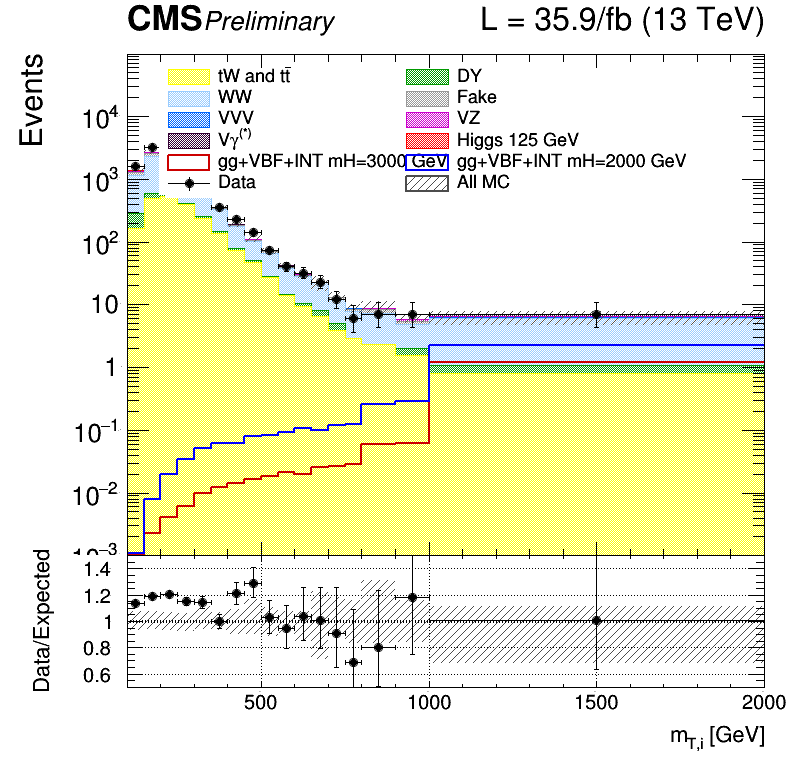
\includegraphics[width=0.45\textwidth]{../Cap5/log_cratio_hwwhm_13TeV_of0j_mTi.png}
}
\subfigure[1 jet]{
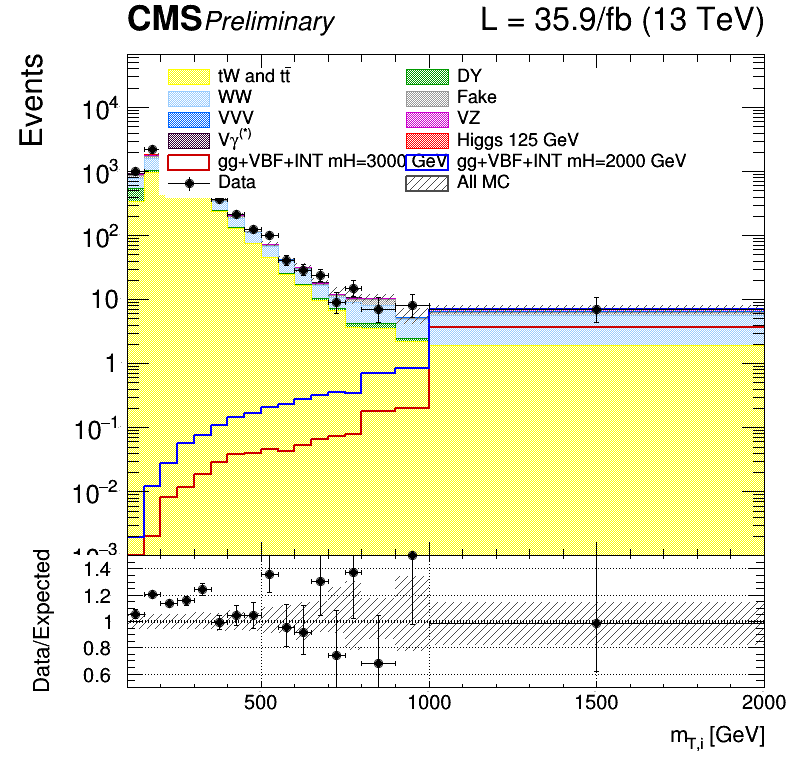
\includegraphics[width=0.45\textwidth]{../Cap5/log_cratio_hwwhm_13TeV_of1j_mTi.png}
}
\\
\subfigure[2 jet]{
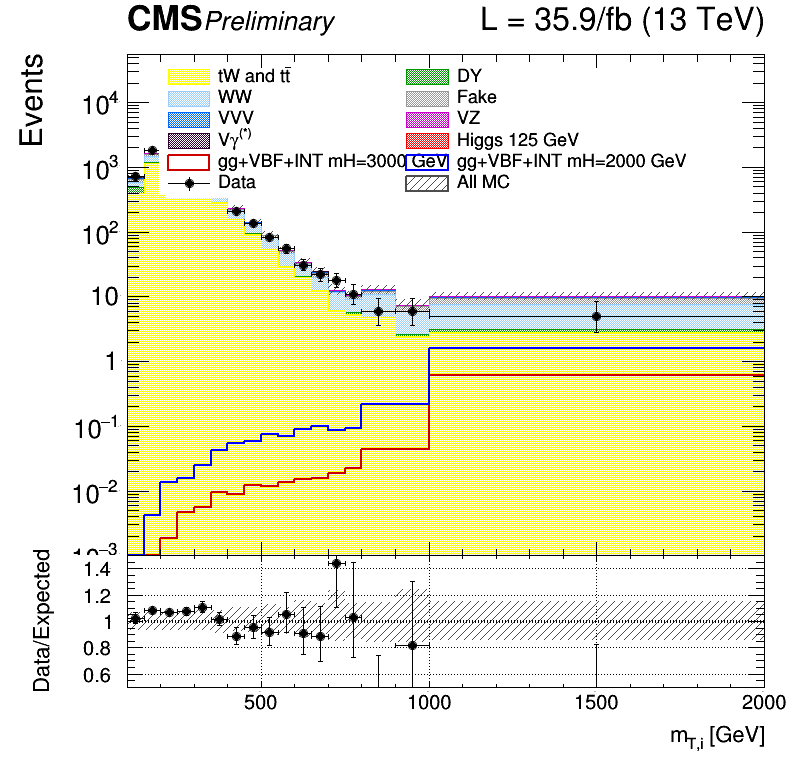
\includegraphics[width=0.45\textwidth]{../Cap5/log_cratio_hwwhm_13TeV_of2j_mTi.png}
}
\subfigure[VBF]{
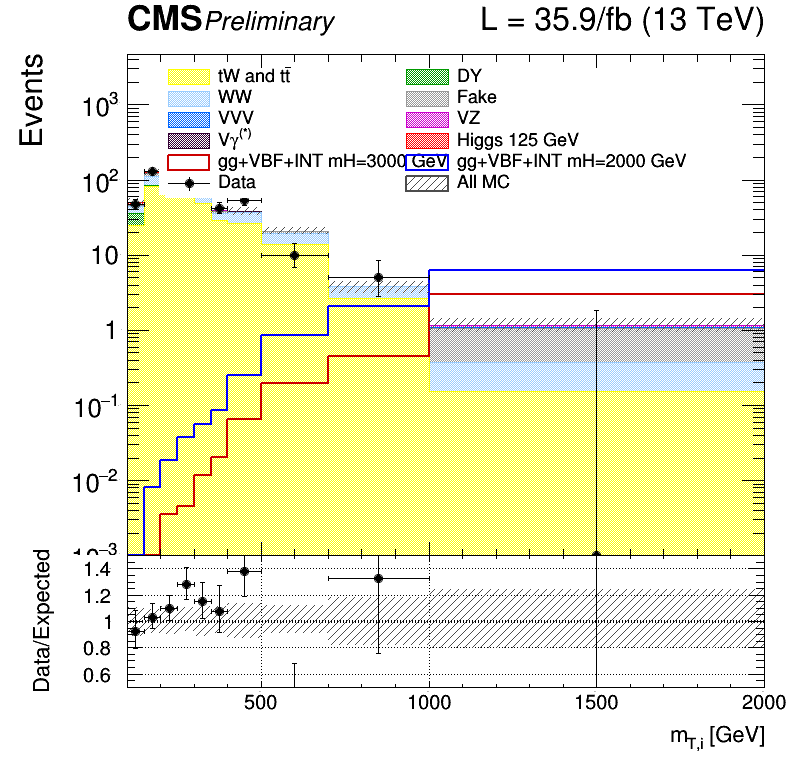
\includegraphics[width=0.45\textwidth]{../Cap5/log_cratio_hwwhm_13TeV_ofVBF_mTi_VBF}
}
\caption{Unblinding distributions  $m_T^I$ in the signal region for 0, 1, 2 and VBF categories. The signal hypothesis corresponding to $m_X $ of 2 and 3 TeV.}
    \label{fig:mti_sigOF_Un_log}
\end{figure}

\newpage
\subsection*{Drell-Yan $\tau\tau$ control region}
To normalize the Drell-Yan $\tau\tau$ background to the data, control regions
have been defined, as close as possible to the signal region, but enriched in
Z $\rightarrow \tau^+ \tau^-$. In particular, the ``WW OF selection'' is used with
inverted $m_T^H$ cut, i.e. $m_T^H<60$. In addition a cut on the invariant mass
of the two leptons 50 GeV $< m_{\ell \ell} <$ 80 GeV is requested to exclude
possible contribution from non-prompt leptons (low limit) and from  $t \bar{t}$ (high
limit).
For each signal category, a corresponding Drell-Yan $\tau\tau$ control
regions is defined. We thus have 4 total  Drell-Yan $\tau\tau$ control
regions, for 0 jets, 1 jets, 2 jets and VBF.
The control plots for several variables in a Drell-Yan enriched phase space
for the four jets categories are shown in Figs.~\ref{fig:CR_DY_OF_0},
~\ref{fig:CR_DY_OF_1}, ~\ref{fig:CR_DY_OF_2}, ~\ref{fig:CR_DY_OF_VBF}.
In general there is a good agreement between data and MC.\\
\begin{figure}[htbp]
\centering
\subfigure[$m_T^I$]{
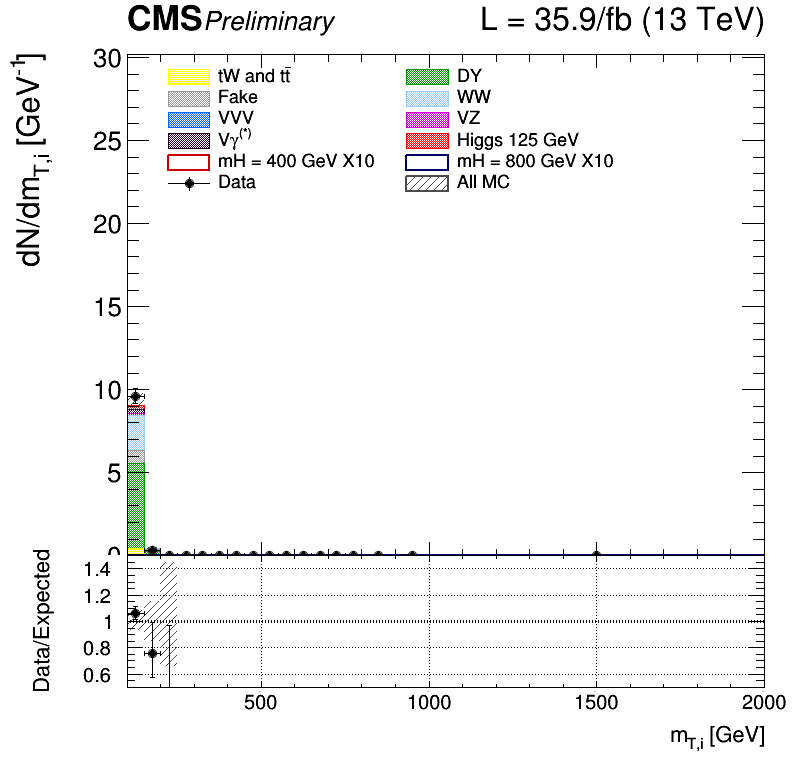
\includegraphics[width=0.45\textwidth]{../AN/Figs/OF_CR_Blind/cratio_hww2l2v_13TeV_dytt_of0j_mTi.png}
}
\subfigure[$m_T^H$]{
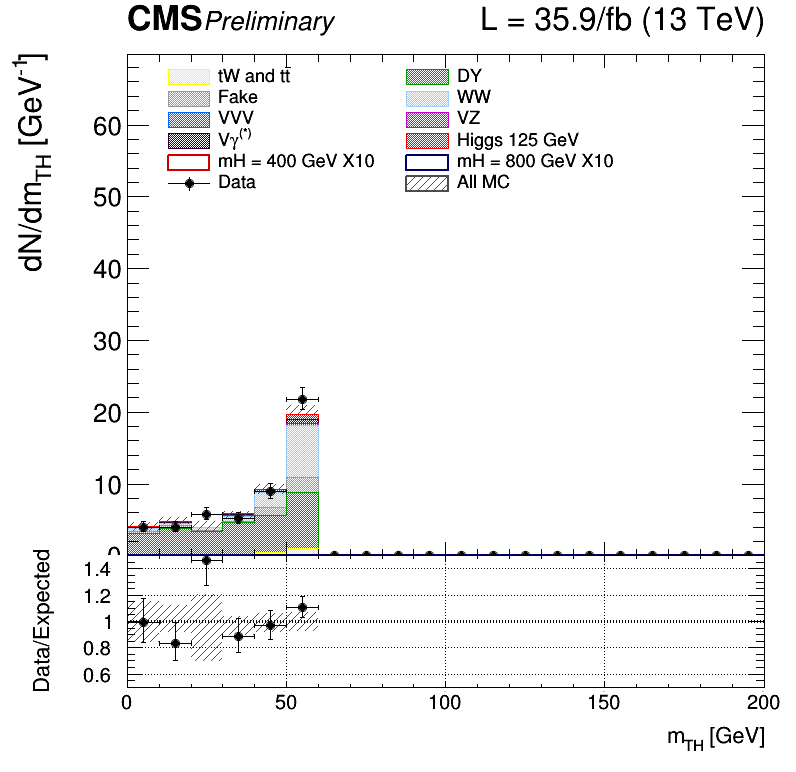
\includegraphics[width=0.45\textwidth]{../AN/Figs/OF_CR_Blind/cratio_hww2l2v_13TeV_dytt_of0j_mth_DY.png}
}                                              
\\                                             
\subfigure[$m_{jj}$]{                             
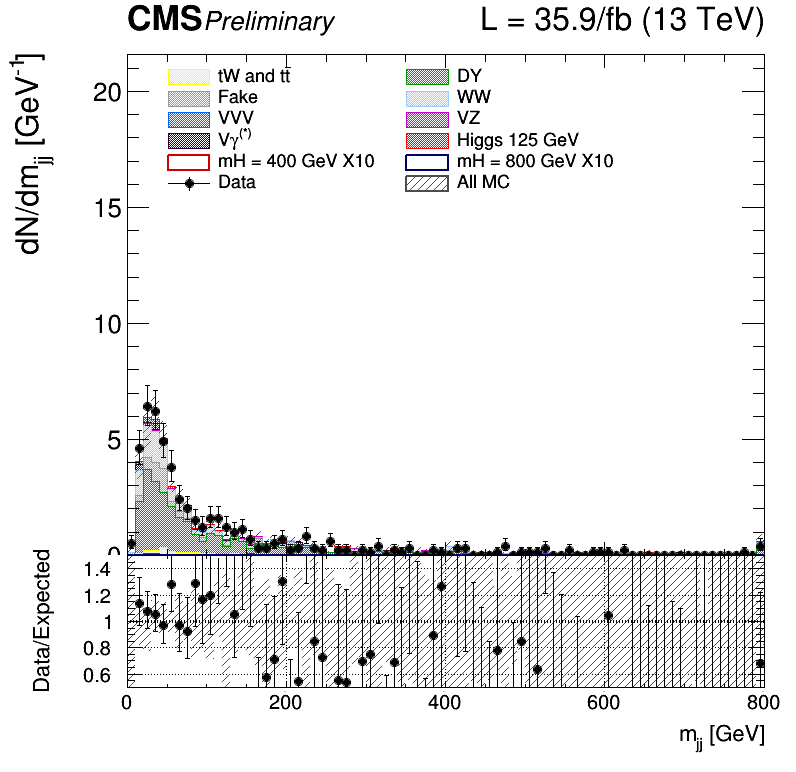
\includegraphics[width=0.45\textwidth]{../AN/Figs/OF_CR_Blind/cratio_hww2l2v_13TeV_dytt_of0j_mjj.png}
}                                              
\subfigure[$m_{\ell \ell}$]{                               
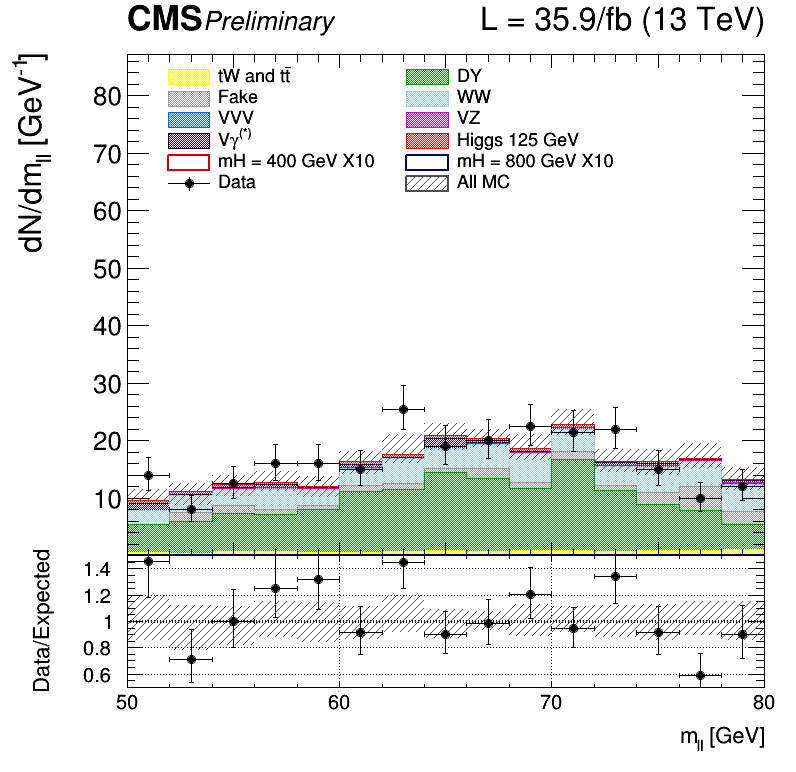
\includegraphics[width=0.45\textwidth]{../AN/Figs/OF_CR_Blind/cratio_hww2l2v_13TeV_dytt_of0j_mll_DY.png}
}\\

\subfigure[$p_T$ leading lepton]{                             
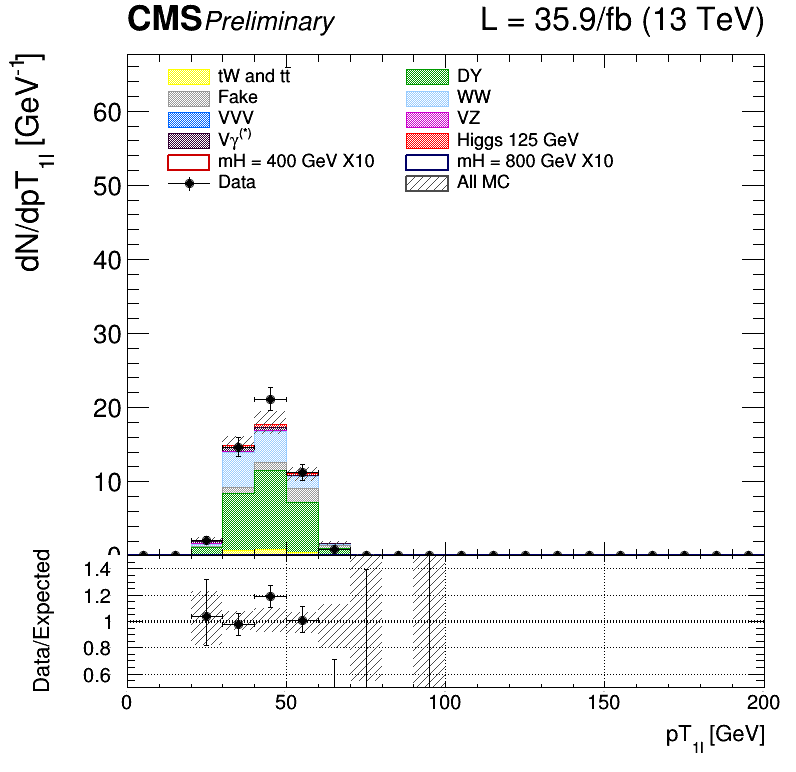
\includegraphics[width=0.45\textwidth]{../AN/Figs/OF_CR_Blind/cratio_hww2l2v_13TeV_dytt_of0j_std_vector_lepton_pt[0].png}
}                                              
\subfigure[$p_T^{\ell \ell}$]{                               
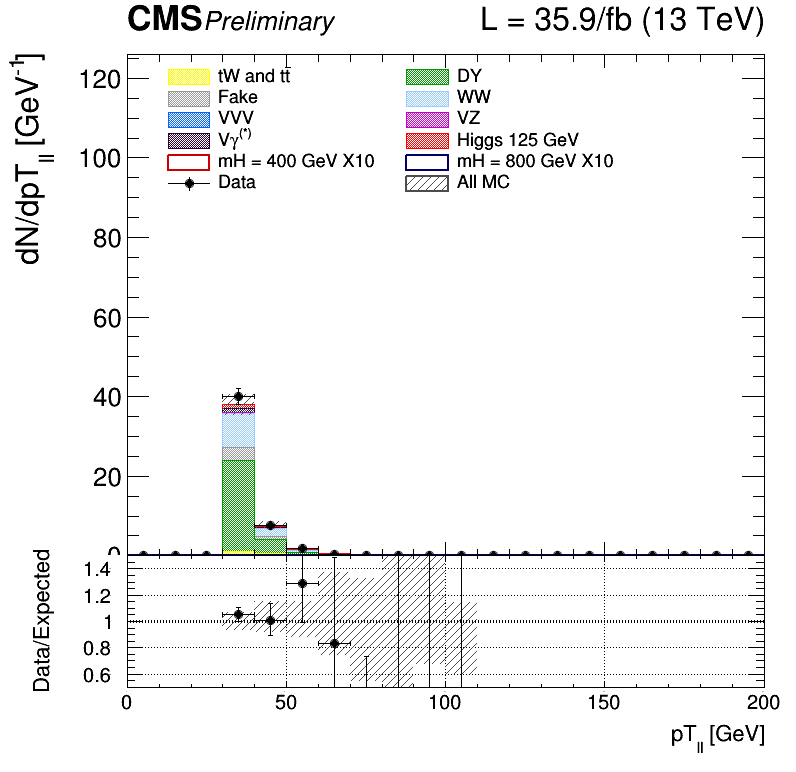
\includegraphics[width=0.45\textwidth]{../AN/Figs/OF_CR_Blind/cratio_hww2l2v_13TeV_dytt_of0j_ptll.png}
}\\

\caption{Control plots for several variables in a Drell-Yan enriched phase space for events with 0 jet.}
    \label{fig:CR_DY_OF_0}
\end{figure}


\begin{figure}[htbp]
\centering
\subfigure[$m_T^I$]{
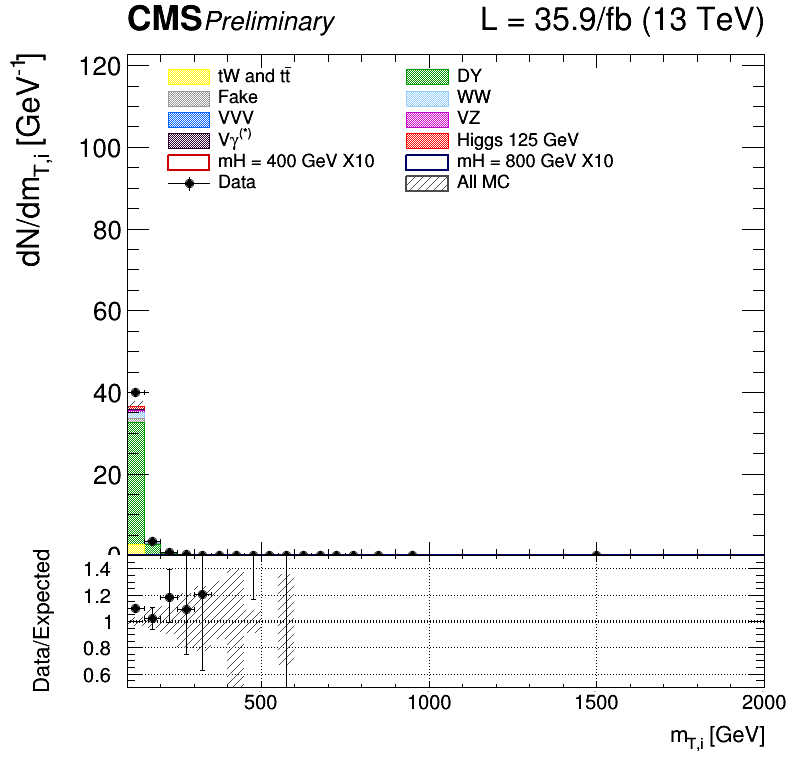
\includegraphics[width=0.45\textwidth]{../AN/Figs/OF_CR_Blind/cratio_hww2l2v_13TeV_dytt_of1j_mTi.png}
}
\subfigure[$m_T^H$]{
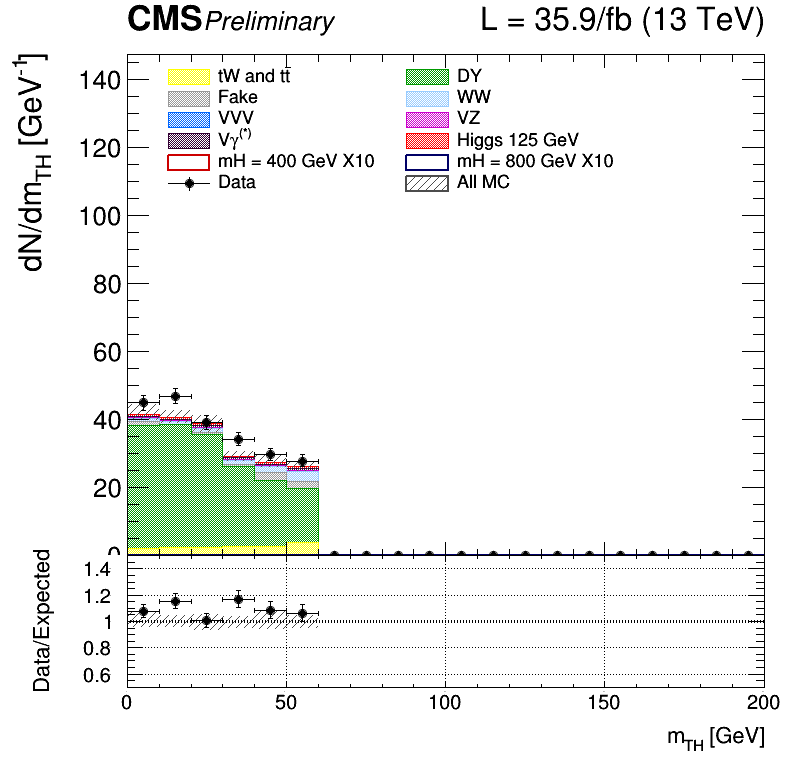
\includegraphics[width=0.45\textwidth]{../AN/Figs/OF_CR_Blind/cratio_hww2l2v_13TeV_dytt_of1j_mth_DY.png}
}                                              
\\                                             
\subfigure[$m_{jj}$]{                             
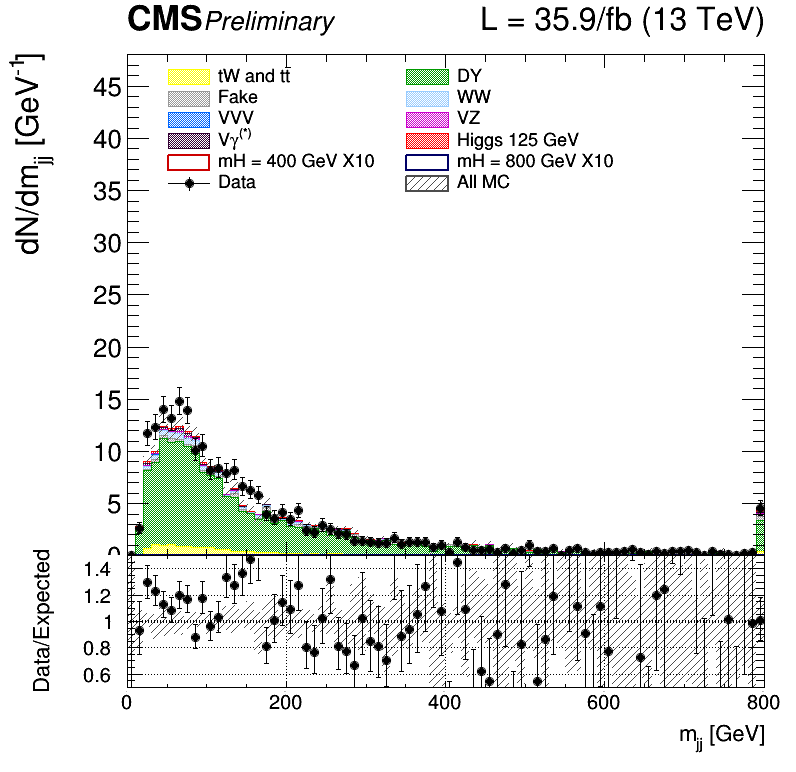
\includegraphics[width=0.45\textwidth]{../AN/Figs/OF_CR_Blind/cratio_hww2l2v_13TeV_dytt_of1j_mjj.png}
}                                              
\subfigure[$m_{\ell \ell}$]{                               
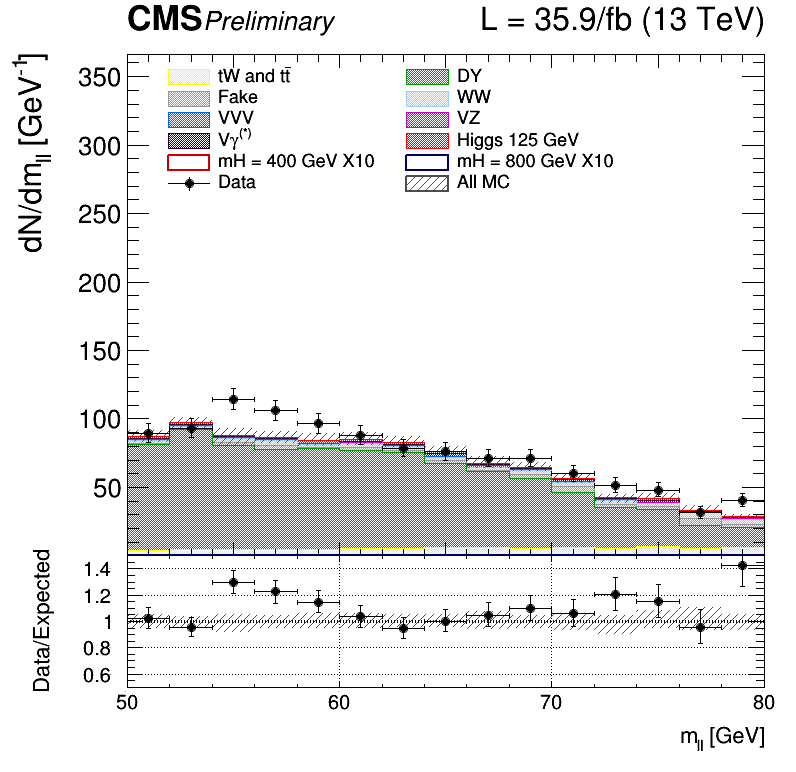
\includegraphics[width=0.45\textwidth]{../AN/Figs/OF_CR_Blind/cratio_hww2l2v_13TeV_dytt_of1j_mll_DY.png}
}\\

\subfigure[$p_T$ leading lepton]{                             
\includegraphics[width=0.45\textwidth]{../AN/Figs/OF_CR_Blind/cratio_hww2l2v_13TeV_dytt_of1j_std_vector_lepton_pt[0].png}
}                                              
\subfigure[$p_T^{\ell \ell}$]{                               
\includegraphics[width=0.45\textwidth]{../AN/Figs/OF_CR_Blind/cratio_hww2l2v_13TeV_dytt_of1j_ptll.png}
}\\

\caption{Control plots for several variables in a Drell-Yan enriched phase space for events with 1 jet.}
    \label{fig:CR_DY_OF_1}
\end{figure}

\begin{figure}[htbp]
\centering
\subfigure[$m_T^I$]{
\includegraphics[width=0.45\textwidth]{../AN/Figs/OF_CR_Blind/cratio_hww2l2v_13TeV_dytt_of2j_mTi.png}
}
\subfigure[$m_T^H$]{
\includegraphics[width=0.45\textwidth]{../AN/Figs/OF_CR_Blind/cratio_hww2l2v_13TeV_dytt_of2j_mth_DY.png}
}                                              
\\                                             
\subfigure[$m_{jj}$]{                             
\includegraphics[width=0.45\textwidth]{../AN/Figs/OF_CR_Blind/cratio_hww2l2v_13TeV_dytt_of2j_mjj.png}
}                                              
\subfigure[$m_{\ell \ell}$]{                               
\includegraphics[width=0.45\textwidth]{../AN/Figs/OF_CR_Blind/cratio_hww2l2v_13TeV_dytt_of2j_mll_DY.png}
}\\

\subfigure[$p_T$ leading lepton]{                             
\includegraphics[width=0.45\textwidth]{../AN/Figs/OF_CR_Blind/cratio_hww2l2v_13TeV_dytt_of2j_std_vector_lepton_pt[0].png}
}                                              
\subfigure[$p_T^{\ell \ell}$]{                               
\includegraphics[width=0.45\textwidth]{../AN/Figs/OF_CR_Blind/cratio_hww2l2v_13TeV_dytt_of2j_ptll.png}
}\\

\caption{Control plots for several variables in a Drell-Yan enriched phase space for events with 2 jet.}
    \label{fig:CR_DY_OF_2}
\end{figure}




\begin{figure}[htbp]
\centering
\subfigure[$m_T^I$]{
\includegraphics[width=0.45\textwidth]{../AN/Figs/OF_CR_Blind/cratio_hww2l2v_13TeV_dytt_of2j_vbf_mTi.png}
}
\subfigure[$m_T^H$]{
\includegraphics[width=0.45\textwidth]{../AN/Figs/OF_CR_Blind/cratio_hww2l2v_13TeV_dytt_of2j_vbf_mth_DY.png}
}                                              
\\                                             
\subfigure[$m_{jj}$]{                             
\includegraphics[width=0.45\textwidth]{../AN/Figs/OF_CR_Blind/cratio_hww2l2v_13TeV_dytt_of2j_vbf_mjj_DY_VBF.png}
}                                              
\subfigure[$m_{\ell \ell}$]{                               
\includegraphics[width=0.45\textwidth]{../AN/Figs/OF_CR_Blind/cratio_hww2l2v_13TeV_dytt_of2j_vbf_mll_DY.png}
}\\

\subfigure[$p_T$ leading lepton]{                             
\includegraphics[width=0.45\textwidth]{../AN/Figs/OF_CR_Blind/cratio_hww2l2v_13TeV_dytt_of2j_vbf_std_vector_lepton_pt[0].png}
}                                              
\subfigure[$p_T^{\ell \ell}$]{                               
\includegraphics[width=0.45\textwidth]{../AN/Figs/OF_CR_Blind/cratio_hww2l2v_13TeV_dytt_of2j_vbf_ptll.png}
}\\

\caption{Control plots for several variables in a Drell-Yan enriched phase space for events for VBF.}
    \label{fig:CR_DY_OF_VBF}
\end{figure}



\newpage
\subsection*{Top control region}
Similarly to the Drell-Yan $\tau\tau$ case, control regions are defined for the Top
background, and they are used to normalize the top background to data.
The ``WW OF selection'' is used with inversion of the veto on b-jets. In
particular the following conditions are imposed to select a top enriched
control region for each of the 4 signal regions:
\begin{itemize}
\item {\bf 0 jet}, at least one b-tagged jet with 20 $< p_T <$ 30 GeV is required;
\item {\bf 1 jet}, exactly one b-tagged jet with $p_T$ above 30 GeV is required;
\item {\bf 2 jet}, exacly 2 jets with at least one of them b-tagged and in addition the condition $\Delta \eta_{jj} < 3.5$ {\bf or} $m_{jj} <$ 500 GeV;
\item {\bf VBF}, exacly 2 jets with at least one of them b-tagged and in addition the condition $\Delta \eta_{jj} > 3.5$ {\bf and} $m_{jj} >$ 500 GeV.
\end{itemize}
A jet is considered b-tagged if its cMVAv2 score is above the threshold
defining the loose working point.
The control plots for several variables in a top enriched phase space for events are shown in the Fig.~ Figs.~\ref{fig:Top_0j},~\ref{fig:Top_1j},~\ref{fig:Top_2j},~\ref{fig:Top_VBF}. The last bin in the distribution is the overflow.
\begin{figure}[htbp]
\centering
\subfigure[$m_T^I$]{
\includegraphics[width=0.45\textwidth]{../AN/Figs/OF_CR_Blind/cratio_hww2l2v_13TeV_top_of0j_mTi.png}
}
\subfigure[$m_T^H$]{
\includegraphics[width=0.45\textwidth]{../AN/Figs/OF_CR_Blind/cratio_hww2l2v_13TeV_top_of0j_mth.png}
}                                              
\\                                             
\subfigure[$m_{jj}$]{                             
\includegraphics[width=0.45\textwidth]{../AN/Figs/OF_CR_Blind/cratio_hww2l2v_13TeV_top_of0j_mjj.png}
}                                              
\subfigure[$m_{\ell \ell}$]{                               
\includegraphics[width=0.45\textwidth]{../AN/Figs/OF_CR_Blind/cratio_hww2l2v_13TeV_top_of0j_mll.png}
}\\

\subfigure[$p_T$ leading lepton]{                             
\includegraphics[width=0.45\textwidth]{../AN/Figs/OF_CR_Blind/cratio_hww2l2v_13TeV_top_of0j_std_vector_lepton_pt[0].png}
}                                              
\subfigure[$p_T^{\ell \ell}$]{                               
\includegraphics[width=0.45\textwidth]{../AN/Figs/OF_CR_Blind/cratio_hww2l2v_13TeV_top_of0j_ptll.png}
}\\

\caption{Control plots for several variables in the Top enriched phase space for events with 0 jet.}
    \label{fig:Top_0j}
\end{figure}




\begin{figure}[htbp]
\centering
\subfigure[$m_T^I$]{
\includegraphics[width=0.45\textwidth]{../AN/Figs/OF_CR_Blind/cratio_hww2l2v_13TeV_top_of1j_mTi.png}
}
\subfigure[$m_T^H$]{
\includegraphics[width=0.45\textwidth]{../AN/Figs/OF_CR_Blind/cratio_hww2l2v_13TeV_top_of1j_mth.png}
}                                              
\\                                             
\subfigure[$m_{jj}$]{                             
\includegraphics[width=0.45\textwidth]{../AN/Figs/OF_CR_Blind/cratio_hww2l2v_13TeV_top_of1j_mjj.png}
}                                              
\subfigure[$m_{\ell \ell}$]{                               
\includegraphics[width=0.45\textwidth]{../AN/Figs/OF_CR_Blind/cratio_hww2l2v_13TeV_top_of1j_mll.png}
}\\

\subfigure[$p_T$ leading lepton]{                             
\includegraphics[width=0.45\textwidth]{../AN/Figs/OF_CR_Blind/cratio_hww2l2v_13TeV_top_of1j_std_vector_lepton_pt[0].png}
}                                              
\subfigure[$p_T^{\ell \ell}$]{                               
\includegraphics[width=0.45\textwidth]{../AN/Figs/OF_CR_Blind/cratio_hww2l2v_13TeV_top_of1j_ptll.png}
}\\

\caption{Control plots for several variables in the Top enriched phase space for events with 1 jet.}
    \label{fig:Top_1j}
\end{figure}



\begin{figure}[htbp]
\centering
\subfigure[$m_T^I$]{
\includegraphics[width=0.45\textwidth]{../AN/Figs/OF_CR_Blind/cratio_hww2l2v_13TeV_top_of2j_mTi.png}
}
\subfigure[$m_T^H$]{
\includegraphics[width=0.45\textwidth]{../AN/Figs/OF_CR_Blind/cratio_hww2l2v_13TeV_top_of2j_mth.png}
}                                              
\\                                             
\subfigure[$m_{jj}$]{                             
\includegraphics[width=0.45\textwidth]{../AN/Figs/OF_CR_Blind/cratio_hww2l2v_13TeV_top_of2j_mjj.png}
}                                              
\subfigure[$m_{\ell \ell}$]{                               
\includegraphics[width=0.45\textwidth]{../AN/Figs/OF_CR_Blind/cratio_hww2l2v_13TeV_top_of2j_mll.png}
}\\

\subfigure[$p_T$ leading lepton]{                             
\includegraphics[width=0.45\textwidth]{../AN/Figs/OF_CR_Blind/cratio_hww2l2v_13TeV_top_of2j_std_vector_lepton_pt[0].png}
}                                              
\subfigure[$p_T^{\ell \ell}$]{                               
\includegraphics[width=0.45\textwidth]{../AN/Figs/OF_CR_Blind/cratio_hww2l2v_13TeV_top_of2j_ptll.png}
}\\

\caption{Control plots for several variables in the Top enriched phase space for events with 2 jet.}
    \label{fig:Top_2j}
\end{figure}



\begin{figure}[htbp]
\centering
\subfigure[$m_T^I$]{
\includegraphics[width=0.45\textwidth]{../AN/Figs/OF_CR_Blind/cratio_hww2l2v_13TeV_top_VBF_mTi.png}
}
\subfigure[$m_T^H$]{
\includegraphics[width=0.45\textwidth]{../AN/Figs/OF_CR_Blind/cratio_hww2l2v_13TeV_top_VBF_mth.png}
}                                              
\\                                             
\subfigure[$m_{jj}$]{                             
\includegraphics[width=0.45\textwidth]{../AN/Figs/OF_CR_Blind/cratio_hww2l2v_13TeV_top_VBF_mjj_DY_VBF.png}
}                                              
\subfigure[$m_{\ell \ell}$]{                               
\includegraphics[width=0.45\textwidth]{../AN/Figs/OF_CR_Blind/cratio_hww2l2v_13TeV_top_VBF_mll.png}
}\\

\subfigure[$p_T$ leading lepton]{                             
\includegraphics[width=0.45\textwidth]{../AN/Figs/OF_CR_Blind/cratio_hww2l2v_13TeV_top_VBF_std_vector_lepton_pt[0].png}
}                                              
\subfigure[$p_T^{\ell \ell}$]{                               
\includegraphics[width=0.45\textwidth]{../AN/Figs/OF_CR_Blind/cratio_hww2l2v_13TeV_top_VBF_ptll.png}
}\\

\caption{Control plots for several variables in the Top enriched phase space for events in VBF region.}
    \label{fig:Top_VBF}
\end{figure}


\clearpage

% ---- ---- ---- ---- ---- ---- ---- ---- ---- ---- ---- ---- ---- ---- ---- ---- ----
\newpage
\section{Same Flavor final state}\label{sec:SF}
The analysis if the same-flavour final state $\mathrm{W^+W^-}\to \mu^{\pm}
\mu^{\mp}  2\nu$ and  $\mathrm{W^+W^-}\to e^{\pm} e^{\mp}  2\nu$ is described.
\subsection*{Signal region}
Events are requested to pass single or double lepton triggers and all the
physics objects definitions are the same as in the OF analysis.
The final state consists of two well identified electrons or two muons with
$p_T >$ 20 GeV, opposite charge, and large missing transverse energy from the undetected neutrinos.\\
In addition to the backgrounds described for the OF final state, the
background from $\mathrm{DY}\to \mu^{+} \mu^{-}$ and
$\mathrm{DY}\to e^{+} e^{-}$ is very large in this final state.
Indeed, due to this very large background, the SF analysis only targets the
VBF topology, where the DY background is suppressed by the tight 
jet requirements. In addition, an invariant mass of the two leptons larger
than 120~\GeV is requested.
The full selection, defined as the ``WW same flavour selection'', is :
\begin{itemize}
\item Two isolated leptons with same flavor and opposite charge ($\mu ^{\pm} \mu^{\mp}$ and $e^{\pm} e^{\mp}$);
\item $p_T$ of the leading and trailing lepton $>$ 20 GeV;
\item Third lepton veto: veto events if a third lepton with $p_T  >$ 10 GeV;
\item  $m_{\ell \ell} >$ 120 GeV 
\item $p_T^{\ell \ell} >$30 GeV;
\item MET $>$ 50 GeV;
\item $m_T^I >$ 100 GeV;
\item At lest 2 jets non b-tagged (according to cMVAv2 loose WP) with $p_T >$ 30 GeV.
\item $\Delta \eta_{jj} > 3.5$;
\item $m_{jj} >$ 500 GeV;;
\end{itemize}
Similarly to the opposite-flavour analysis, the signal is extracted from a template fit of
the $m_T^I$ distribution.
The $m_T^I$ distributions has the following binning:
\begin{itemize}
\item {\bf VBF}, [100,150,200,250,300,350,400,450,500,600,700,1000];
\end{itemize}
where the first number represents the lower edge of the first bin while the other numbers represent the upper edges. The last bin is an overflow bin. 
The binning has been chosen in order to have at least 10 expected Top-backgrounds event and at least 10  expected  Drell-Yan events in each bin of the template.\\
The distributions for the signal region of $m_T^I$ variable is shown in  Fig.~\ref{fig:mti_sigOF_Un_log} 
\begin{figure}[htbp]
\centering
\subfigure[ee]{
\includegraphics[width=0.45\textwidth]{../AN/Figs/unblinding/plot_SR/plotHWWhighMass_SF_ee_postfit_300/cratio_hwwhm_13TeV_sfVBF_ee_mTi.png}
}
\subfigure[mm]{
\includegraphics[width=0.45\textwidth]{../AN/Figs/unblinding/plot_SR/plotHWWhighMass_SF_mm_postfit_300/cratio_hwwhm_13TeV_sfVBF_mm_mTi.png}
}
\\
\subfigure[ee]{
\includegraphics[width=0.45\textwidth]{../AN/Figs/unblinding/plot_SR/plotHWWhighMass_SF_ee_postfit_300/log_cratio_hwwhm_13TeV_sfVBF_ee_mTi.png}
}
\subfigure[mm]{
\includegraphics[width=0.45\textwidth]{../AN/Figs/unblinding/plot_SR/plotHWWhighMass_SF_mm_postfit_300/log_cratio_hwwhm_13TeV_sfVBF_mm_mTi.png}
}
\caption{Unblinding distributions  $m_T^I$ in the signal region for $ee$ and $\mu \mu$ categories in linear and log scale. The signal hypothesis corresponding to $m_X $ of 300 GeV.}
    \label{fig:mti_sigOF_Un}
\end{figure}




\newpage

\subsection*{Drell-Yan control region}
The main background for the SF analysis is the DY. 
A control region has been defined, as close as possible to the signal one to
be used for the normalization of the DY background, separately for electrons
an muons.
The control region is defined by the ``WW same flavour selection'', except for the
$m_{\ell \ell}$ requirement which is changed to 70 GeV $ <m_{\ell \ell} <$ 120
GeV to include the Z boson.
The missing transverse energy distribution in the data shows discrepancies respect to Monte Carlo simulation  in ee and $\mu \mu$ Drell-Yan control regions. A correction is applied re-weighting all the simulated samples with a weight per event which depends on the MET value. 
The weight is evaluated as the ratio between data, one subtracted all backgrounds except the DY, and the Drell-Yan itself, in each bins of the distribution, separately for ee and $\mu \mu$ categories. The weight is assumed to be linear as function of the MET value.\\
This kind of re-weighting allows to correct for shape differences between data and MC, , Fig. \ref{fig:dy_met}.
The control plots for several variables in a Drell-Yan enriched phase space
for the ee and $\mu \mu$ are shown in Figs.~\ref{fig:mll_sigSF_CR_DY_ee} for
the dielectron case and Figs.~\ref{fig:mll_sigSF_CR_DY_mm} for the dimuon
case. In general there is a good agreement between data and MC.

\newpage

\begin{figure}[htbp]
\centering
\subfigure[ee before the re-weight]{
\includegraphics[width=0.45\textwidth]{../AN/Figs/METrw/cratio_hww2l2v_13TeV_dy_e_e_2j_VBF_metPfType1.png}
}
\subfigure[$\mu \mu$  before the re-weight]{
\includegraphics[width=0.45\textwidth]{../AN/Figs/METrw/cratio_hww2l2v_13TeV_dy_mu_mu_2j_VBF_metPfType1.png}
}                                              

\subfigure[ee  after the re-weight]{
\includegraphics[width=0.45\textwidth]{../AN/Figs/SF_CR_Blind/cratio_hww2l2v_13TeV_dy_e_e_2j_VBF_metPfType1.png}
}
\subfigure[$\mu \mu$  after the re-weight]{
\includegraphics[width=0.45\textwidth]{../AN/Figs/SF_CR_Blind/cratio_hww2l2v_13TeV_dy_mu_mu_2j_VBF_metPfType1.png}
}                   

\caption{MET control plots for Drell-Yan for ee categories in \textit{a} and for $\mu \mu$ in \textit{b} before the re-weight. In \textit{c} and  \textit{d} the same 
distribution after the correction.}
    \label{fig:dy_met}                                             

\end{figure}




\newpage

\begin{figure}[htbp]
\centering
\subfigure[$m_T^I$]{
\includegraphics[width=0.45\textwidth]{../AN/Figs/SF_CR_Blind/cratio_hww2l2v_13TeV_dy_e_e_2j_VBF_mTi.png}
}
\subfigure[$m_T^H$]{
\includegraphics[width=0.45\textwidth]{../AN/Figs/SF_CR_Blind/cratio_hww2l2v_13TeV_dy_e_e_2j_VBF_mth.png}
}                                              
\\                                             
\subfigure[$m_{jj}$]{                             
\includegraphics[width=0.45\textwidth]{../AN/Figs/SF_CR_Blind/cratio_hww2l2v_13TeV_dy_e_e_2j_VBF_mjj_DY.png}
}                                              
\subfigure[$m_{\ell \ell}$]{                               
\includegraphics[width=0.45\textwidth]{../AN/Figs/SF_CR_Blind/cratio_hww2l2v_13TeV_dy_e_e_2j_VBF_mll.png}
}\\

\subfigure[$p_T$ leading lepton]{                             
\includegraphics[width=0.45\textwidth]{../AN/Figs/SF_CR_Blind/cratio_hww2l2v_13TeV_dy_e_e_2j_VBF_std_vector_lepton_pt[0].png}
}                                              
\subfigure[$p_T^{\ell \ell}$]{                               
\includegraphics[width=0.45\textwidth]{../AN/Figs/SF_CR_Blind/cratio_hww2l2v_13TeV_dy_e_e_2j_VBF_ptll.png}
}\\

\caption{Control plots for several variables in a Drell-Yan enriched phase space for ee.}
    \label{fig:mll_sig}
\end{figure}

\newpage

\begin{figure}[htbp]
\centering
\subfigure[$m_T^I$]{
\includegraphics[width=0.45\textwidth]{../AN/Figs/SF_CR_Blind/cratio_hww2l2v_13TeV_dy_e_e_2j_VBF_mTi.png}
}
\subfigure[$m_T^H$]{
\includegraphics[width=0.45\textwidth]{../AN/Figs/SF_CR_Blind/cratio_hww2l2v_13TeV_dy_e_e_2j_VBF_mth.png}
}                                              
\\                                             
\subfigure[$m_{jj}$]{                             
\includegraphics[width=0.45\textwidth]{../AN/Figs/SF_CR_Blind/cratio_hww2l2v_13TeV_dy_e_e_2j_VBF_mjj_DY.png}
}                                              
\subfigure[$m_{\ell \ell}$]{                               
\includegraphics[width=0.45\textwidth]{../AN/Figs/SF_CR_Blind/cratio_hww2l2v_13TeV_dy_e_e_2j_VBF_mll.png}
}\\

\subfigure[$p_T$ leading lepton]{                             
\includegraphics[width=0.45\textwidth]{../AN/Figs/SF_CR_Blind/cratio_hww2l2v_13TeV_dy_e_e_2j_VBF_std_vector_lepton_pt[0].png}
}                                              
\subfigure[$p_T^{\ell \ell}$]{                               
\includegraphics[width=0.45\textwidth]{../AN/Figs/SF_CR_Blind/cratio_hww2l2v_13TeV_dy_e_e_2j_VBF_ptll.png}
}\\

\caption{Control plots for several variables in a Drell-Yan enriched phase space for ee.}
    \label{fig:mll_sigSF_CR_DY_ee}
\end{figure}


\newpage

\begin{figure}[h]
\centering
\subfigure[$m_T^I$]{
\includegraphics[width=0.45\textwidth]{../AN/Figs/SF_CR_Blind/cratio_hww2l2v_13TeV_dy_mu_mu_2j_VBF_mTi.png}
}
\subfigure[$m_T^H$]{
\includegraphics[width=0.45\textwidth]{../AN/Figs/SF_CR_Blind/cratio_hww2l2v_13TeV_dy_mu_mu_2j_VBF_mth.png}
}                                              
\\                                             
\subfigure[$m_{jj}$]{                             
\includegraphics[width=0.45\textwidth]{../AN/Figs/SF_CR_Blind/cratio_hww2l2v_13TeV_dy_mu_mu_2j_VBF_mjj_DY.png}
}                                              
\subfigure[$m_{\ell \ell}$]{                               
\includegraphics[width=0.45\textwidth]{../AN/Figs/SF_CR_Blind/cratio_hww2l2v_13TeV_dy_mu_mu_2j_VBF_mll.png}
}\\

\subfigure[$p_T$ leading lepton]{                             
\includegraphics[width=0.45\textwidth]{../AN/Figs/SF_CR_Blind/cratio_hww2l2v_13TeV_dy_mu_mu_2j_VBF_std_vector_lepton_pt[0].png}
}                                              
\subfigure[$p_T^{\ell \ell}$]{                               
\includegraphics[width=0.45\textwidth]{../AN/Figs/SF_CR_Blind/cratio_hww2l2v_13TeV_dy_mu_mu_2j_VBF_ptll.png}
}\\

\caption{Control plots for several variables in a Drell-Yan enriched phase space for $\mu \mu$.}
    \label{fig:mll_sigSF_CR_DY_mm}
\end{figure}

\newpage
\clearpage
\subsection*{Top control region}
A top-enriched control region is defined to normalize the top backgrounds,
separately for electrons and muons.
The ``WW SF selection'' is required with the inversion of the b-tagging
requirement, i.e. the two jets are both requested to be b-tagged according to
cMVAv2 loose WP.
The control plots for several variables in a top enriched phase space for events are shown in
the Figs.~\ref{fig:mll_sigSF_CR_top_ee} for the dielectron case and
\ref{fig:mll_sigSF_CR_top_mm} for the dimuon case. Good agreement is observed
between data and MC.


\begin{figure}[htbp]
\centering
\subfigure[$m_T^I$]{
\includegraphics[width=0.45\textwidth]{../AN/Figs/SF_CR_Blind/cratio_hww2l2v_13TeV_top_e_e_2j_VBF_mTi.png}
}
\subfigure[$m_T^H$]{
\includegraphics[width=0.45\textwidth]{../AN/Figs/SF_CR_Blind/cratio_hww2l2v_13TeV_top_e_e_2j_VBF_mth.png}
}                                              
\\                                             
\subfigure[$m_{jj}$]{                             
\includegraphics[width=0.45\textwidth]{../AN/Figs/SF_CR_Blind/cratio_hww2l2v_13TeV_top_e_e_2j_VBF_mjj_DY.png}
}                                              
\subfigure[$m_{\ell \ell}$]{                               
\includegraphics[width=0.45\textwidth]{../AN/Figs/SF_CR_Blind/cratio_hww2l2v_13TeV_top_e_e_2j_VBF_mll_DY.png}
}\\

\subfigure[$p_T$ leading lepton]{                             
\includegraphics[width=0.45\textwidth]{../AN/Figs/SF_CR_Blind/cratio_hww2l2v_13TeV_top_e_e_2j_VBF_std_vector_lepton_pt[0].png}
}                                              
\subfigure[$p_T^{\ell \ell}$]{                               
\includegraphics[width=0.45\textwidth]{../AN/Figs/SF_CR_Blind/cratio_hww2l2v_13TeV_top_e_e_2j_VBF_njet.png}
}\\

\caption{Control plots for several variables in a Top enriched phase space for ee.}
    \label{fig:mll_sigSF_CR_top_ee}
\end{figure}




\begin{figure}[htbp]
\centering
\subfigure[$m_T^I$]{
\includegraphics[width=0.45\textwidth]{../AN/Figs/SF_CR_Blind/cratio_hww2l2v_13TeV_top_mu_mu_2j_VBF_mTi.png}
}
\subfigure[$m_T^H$]{
\includegraphics[width=0.45\textwidth]{../AN/Figs/SF_CR_Blind/cratio_hww2l2v_13TeV_top_mu_mu_2j_VBF_mth.png}
}                                              
\\                                             
\subfigure[$m_{jj}$]{                             
\includegraphics[width=0.45\textwidth]{../AN/Figs/SF_CR_Blind/cratio_hww2l2v_13TeV_top_mu_mu_2j_VBF_mjj_DY.png}
}                                              
\subfigure[$m_{\ell \ell}$]{                               
\includegraphics[width=0.45\textwidth]{../AN/Figs/SF_CR_Blind/cratio_hww2l2v_13TeV_top_mu_mu_2j_VBF_mll_DY.png}
}\\

\subfigure[$p_T$ leading lepton]{                             
\includegraphics[width=0.45\textwidth]{../AN/Figs/SF_CR_Blind/cratio_hww2l2v_13TeV_top_mu_mu_2j_VBF_std_vector_lepton_pt[0].png}
}                                              
\subfigure[$p_T^{\ell \ell}$]{                               
\includegraphics[width=0.45\textwidth]{../AN/Figs/SF_CR_Blind/cratio_hww2l2v_13TeV_top_mu_mu_2j_VBF_njet.png}
}\\

\caption{Control plots for several variables in a Top enriched phase space for $\mu \mu$.}
    \label{fig:mll_sigSF_CR_top_mm}
\end{figure}



\clearpage

% ---- ---- ---- ---- ---- ---- ---- ---- ---- ---- ---- ---- ---- ---- ---- ---- ----
\newpage
\section{2HDM and MSSM interpretations}\label{sec:2HDM}
In this section the interpretation of this analysis in a Two-Higgs-doublet model (2HDM) and in some scenarios of the Minimal Supersymmetric extension to the Standard Model (MSSM) is described. \\


\subsection{Introduction to 2HDM and MSSM}

The 2HDM is a well motivated extension of the SM. It contains two Higgs doublets, from which a total of five Higgs bosons are predicted: Two CP-even bosons $h$ and $H$, a CP-odd boson $A$ and two charged bosons $H^\pm$. In most theories, $h$ exhibits the features of the SM Higgs boson, while $H$ is a CP-even Higgs boson at a higher mass. In this study, limits are calculated on the production cross section of the Higgs boson $H$ multiplied with the branching fraction of the decay into two $W$ bosons.\newline
The 2HDM comprises many free parameters. Two of these are of particular interest:
\begin{itemize}
\item $\tan\beta$: The ratio $\frac{v_u}{v_d}$ of the vacuum expectation values of the two Higgs doublets.
\item $\alpha$: The mixing angle of the two scalar Higgs bosons $h$ and $H$.
\end{itemize}
The quantity $\cos(\beta-\alpha)$ is also of interest, as the coupling of the heavy scalar Higgs boson $H$ to two vector bosons is proportional to this factor. In the decoupling limit, which occurs at $\cos(\beta-\alpha)=0$, all couplings become SM-like.\newline
A 2HDM of type-2 is considered in this analysis. Here up-type quarks couple to one doublet, while down-type quarks and leptons couple to the other doublet. The MSSM is a type-2 2HDM. On tree level only two parameters are left free. By convention, these parameters are chosen to be $\tan\beta$ and $m_{A}$, the mass of the pseudoscalar Higgs boson. The exclusion limits can be set in a two-dimensional plane as a function of these two parameters. Due to higher order diagrams additional free parameters occur. Benchmark scenarios are then used in order to constrain these parameters. Here two MSSM scenarios are used: The $m_{h}^{mod+}$ scenario and the hMSSM scenario \cite{Carena:2013ytb}.\newline
The analysis follows the same steps as described in sections \ref{sec:OF} and \ref{sec:SF}.

\subsection{Statistical inference}

The necessary model predictions for these scenarios are provided by the LHC Higgs Cross Section Working Group \cite{bsmhiggsxsecs}. For both MSSM scenarios the ggF cross sections have been computed with SusHi (v.1.4.1)\cite{Harlander:2012pb}. These cross sections include NLO supersymmetric QCD corrections and NNLO QCD corrections for the top quark contribution in the effective theory of a heavy top quark, as well as electroweak effects by light quarks. The masses of the Higgs bosons, their mixing, the branching fractions and the effective Yukawa couplings in the $m_{h}^{mod+}$ scenario are all calculated with FeynHiggs (v.2.10.2)\cite{Heinemeyer:1998yj, Heinemeyer:1998np, Degrassi:2002fi, Frank:2006yh, Hahn:2013ria}. For the hMSSM scenario the branching fractions are obtained from HDECAY (v.6.40)\cite{Djouadi:1997yw, Djouadi:2006bz}. The results for general 2HDM are obtained using the ggF cross sections computed with SusHi (v.1.5.0) and the branching fractions from 2HDMC (v.1.7.0)\cite{Rathsman:2011yv}. The VBF cross sections are calculated using an approximation. The BSM Higgs production cross sections for VBF, which are provided for different masses by the LHC Higgs Cross Section Working Group \cite{bsmhiggsxsecs2}, are taken and multiplied by $\cos^{2}(\beta-\alpha)$, resulting in VBF cross sections for a heavy CP-even Higgs boson.\newline
The exclusion limits obtained for the MSSM scenarios are displayed in the $m_{A}$-$\tan\beta$ plane. A fine grid is chosen in this plane, and for each point of this grid a maximum likelihood fit is performed after the $m_{A}$ and/or $\tan\beta$ dependent values of the model, such as cross sections and masses of the Higgs bosons are calculated. These fits are done using the asymptotic method. Performing a maximum likelihood fit in this manner is equivalent to a hypothesis test, where the signal hypothesis is tested against the SM-and-background hypothesis. The signal hypothesis for a combination of $m_{A}$ and $\tan\beta$ is excluded at $95\,\%$ confidence level. In the two-dimensional plane this limit is determined from interpolation between the points of the grid. The limits in the more general 2HDM are obtained in the same way, although a different parameter is chosen in place of $m_{A}$.
\clearpage

% ---- ---- ---- ---- ---- ---- ---- ---- ---- ---- ---- ---- ---- ---- ---- ---- ----
\newpage

\section{Systematic uncertainties}\label{sec:systematics}
Systematic uncertainties are introduced as nuisance parameters in the fit and can affect the
normalization and the shape of the different contributions.

Statistical uncertainties from MC simulated events are taken into account.
Systematic uncertainties are represented by individual nuisance parameters with log-normal or
shape-based distributions. The uncertainties affect the overall normalization of the signal and
backgrounds as well as the shape of the predictions across the distribution of the observables.
Correlations between systematic uncertainties in different categories and final states are taken
into account. Systematic uncertainties play an especially important role in this analysis where
no strong mass peak is expected due to the presence of undetected neutrinos in the final state.
Below we describe in detail sources and quantities of systematics in this analysis and their
effects on the signal and background processes.
A list of the most important background uncertainties is given below.


\subsection*{Background normalization uncertainties}
One of the most important sources of systematic uncertainty is the normalization of the backgrounds that are estimated on data control samples whenever is possible. The signal extraction is performed subtracting the estimated backgrounds to the event counts in data. The amount of uncertainty depends on the considered background:
\begin{itemize}
\item  jet-induced background: normalization and kinematic shapes are derived from a
data control region and both normalization and shape systematic uncertainties are
considered. A conservative 30$\%$ uncertainty on the fake rate is assumed correlated across the different analysis regions. The contribution to the uncertainty in the signal region due to the limited electron statistics in the background enriched control regions is about 10\%, while the contribution due
to the limited muon statistics 3\%. 
\item WW background: The normalization of the WW background is performed independently in each jet multiplicity via the rateParam feature of combine. 
A WW electroweak (VBS) sample is used in addition to the standard WW sample in
the phase spaces with at least two jets, where its contribution becomes non neglgible.
The uncertainty in the cross section for this process is evaluated using the variations
of the renormalization and factorization QCD scales, as well as the PDF variations,
and amounts to 11\%.
\item $\bar{t}t$ and tW backgrounds: Top events are estimated with b-tagging in data control regions. The two top background enriched control regions are defined as additional categories in the fit while the kinematic shapes are taken from the simulation corrected for the b-tagging discriminant scale factors. The top normalization is correlated between the top control region and the Higgs signal categories separately in
the different jet multiplicities, and these normalizations are left unconstrained using the rateParam feature of combine. 
\item Drell-Yan background: The Drell-Yan background enters the different flavor analysis via the leptonic decays of the $\tau$ leptons from $Z \gamma^* \to \tau \tau$. In the different flavor
analyses the normalization of these background is controlled via the rateParam
feature of combine and with a dedicated control region in each jet bin category. 

\item $W \gamma^*$ background: The kinematic shape of this background is predicted by simulation, normalized to its data-driven estimate, and constrained within the respective
uncertainty, which is 25\%.
\item WZ : The kinematic shapes of this backgrounds are predicted by simulation and
normalized to their theoretical predictions in the different and same flavour analysis.

\item $ Z \gamma^*$  : The kinematic shapes of this backgrounds are predicted by simulation and
normalized to their theoretical predictions in the different and same flavor analysis.

\item ZZ: The kinematic shapes of this backgrounds are predicted by simulation and nor-
malized to their theoretical predictions in the different and same flavor analysis.

\end{itemize}




\subsection*{Experimental uncertainties}
Effects from experimental uncertainties are studied by applying a scaling and/or smearing of
certain variables of the physics objects, followed by a subsequent recalculation of all the correlated variables. This is done for MC simulation, to account for possible systematic mismeasurements of the data. All experimental sources except luminosity are treated both as normalization and shape uncertainties. For background with a data-driven normalization estimation,
the shape uncertainty is considered only. The following experimental systematic sources have
been taken into account.

\begin{itemize}
\item Luminosity: The uncertainty determined by the CMS luminosity monitoring is 2.3\% for 13 TeV data.
\item Lepton trigger systematics: Lepton trigger systematics are of the order of less than 1\%. 
These uncertainties are computed by varying the tag selection
as well as the Z window in the tag and probe method used to compute the corresponding scale factors.
\item Lepton reconstruction and identification efficiency:
The lepton reconstruction and identification efficiencies are measured with the tag
and probe method in data. To correct for the difference in the lepton identification
efficiencies between data and MC, data/MC scale factors dependent on \pt and $\eta$ are
applied to the MC. The resulting uncertainty in the signal region is  1\% for electrons
and 2\% for muon.
\item Muon momentum and electron energy scale:  Uncertainties on both the scale and resolution individually amount to  0.6-1\% for electrons 
and  0.2\% for muons. 

\item MET miss modelling: The MET miss measurement is affected by the possible mismeasurement of individual particles addressed above, 
as well as the additional contributions from the pile-up interactions. The effect of the missing transverse momentum resolution on the event selection is studied by propagating each component of the MET uncertainty to the absolute value and direction of MET.

\item Jet energy scale (JES) uncertainties: We estimate this uncertainty
applying the official jet uncertainties on the JES  and compute the variation of the selection efficiency. JES uncertainty affects the
rates in the signal region at the level of  10\%.

\item b-jet misidentification modelling: The uncertainties on the selection of non-b jets is taken into account by looking at
the b-jet misidentification efficiency. The uncertainties on these scale factors need to be taken into account, and are of the
order of a few percent.
\end{itemize}





\subsection*{ Theoretical uncertainties}
\begin{itemize}
\item PDF and higher-order corrections (renormalization and factorization scale): PDF
uncertainties and the missing knowledge on higher-order corrections, evaluated by
means of scale variation, directly affect the cross section, as well as the acceptance
of a simulated process. The uncertainties that arise from using different PDF sets
were obtained by reweighting events with different PDF sets.

\item Underlying event and parton shower modelling: The underlying event (UE) and
parton shower (PS) modelling uncertainties are estimated by comparing samples
interfaced with different parton showers (Pythia vs Herwig) and UE tunes

\item Single top tW and tt ratio: The ratio between the single top and top pair cross section
is varied by the uncertainty on the ratio between their cross sections, calculated con-
sidering scale variations,

\item A QCD and PDF scales for the signal samples at different masses. The uncertainties are taken from the Yellow Report 3 and the same values are used both for the large width hypothesis and for different values of $C'$. The effect of QCD and PDF scale uncertainties on the analysis selection has aslo been taken into account.

\item The categorization of events based on jet multiplicity introduces additional uncertainties related to higher order corrections. These uncertainties are associated to the ggH production mode and are evaluated independently following the recipe described in~\cite{Boughezal:2013oha} and are 5.6\% for the 0-jet and  13\% for the 1-jet and 20\% for the 2-jet and VBF categories.




\end{itemize}



The top background shape is estimated from simulation and corrected using a data driven b-tagging scale factor. The normalization is measured in a top quark enriched control region obtained inverting the b-veto requirement of the signal region. Three control regions are defined, one for each jet bin category. 
A nuisance parameter is added to take into account the effect of the parton shower uncertainty on th top backgorund. \\
The DY background shape is also estimated from simulation and analogously to the Top background, the DY normalization is measured with a data driven technique in three control regions enriched in DY events.\\
A dedicated nuisances for MET reweighting in DY control region is introduced in SF analysis. It is evaluate separately for ee and $\mu \mu$ categories. 
The uncertainty is quote as maximum and minimum best-fit lines of the linear fit.

 \clearpage

% ---- ---- ---- ---- ---- ---- ---- ---- ---- ---- ---- ---- ---- ---- ---- ---- ----

\section{Fully leptonic results}

\subsection*{Electroweak singlet}
The final binned fit is performed using the $m_T^I$ histogram for all signals and the number of events for the backgrounds.
For the oppiste-flavour and same-flavour analysis, for every categories and for every mass point from
200\GeV up to 3\TeV the significance  and the 95\% CL
upper exclusion limit are calculated.
The expected final limit from the combination of the OF and SF analysis are shown in Fig.~\ref{fig:lim_OFSF_comb}. 
This limit represent a 	considerable improvement respect to the high mass search done with 2015 data and the expected limits is compatible with the ATLAS results for a similar analysis, Sec~\ref{NSP} .\\
\begin{figure}[htb]
\centering
\includegraphics[width=0.65\textwidth]{../AN/Figs/unblinding/Limits/c2_FullComb_unbl.png}
\caption{95$\%$ CL exclusion limits,  on the production ggH and VBF cross section times branching fraction as a function of the mass for the  combination of the two analysis OF and SF, in the full mass range.   The red  line represent the predicted cross-section for EW high mass bosons.}
\label{fig:lim_OFSF_comb}
\end{figure}


\subsection*{2HDM results}
In Fig. ~\ref{fig:MSSM} the exclusion limits are shown for the $m_h^{mod+}$ scenario on the left and the hMSSM scenario on the right. The dashed line marks the limit, while the green area shows the side of the limit that is excluded. The bands surrounding the limit indicate the $\pm 1,2\sigma$ contours. For both scenarios the region at low values of $m_{A}$ and $\tan\beta$ is excluded. These results complement well with the exclusion limit given by the MSSM $H\rightarrow\tau\tau$ analysis, where the sensitivity is lower for low $m_{A}$ and $\tan\beta$.

\begin{figure}[htb]
\centering
\subfigure[$m_h^{mod+}$]{
\includegraphics[width=0.45\textwidth]{../AN/Figs/unblinding/2HDM/mhmodp.png}
}
\subfigure[hMSSM]{
\includegraphics[width=0.45\textwidth]{../AN/Figs/unblinding/2HDM/hmssm.png}
}

\caption{95$\%$ CL exclusion limits on the MSSM $m_h^{mod+}$ scenario (left) and the hMSSM scenario (right).}
    \label{fig:MSSM}
\end{figure}

In Fig. ~\ref{fig:2HDM1} and ~\ref{fig:2HDM2} the exclusion limits are shown for a 2HDM. The limits in ~\ref{fig:2HDM1} for both a type-1 and type-2 2HDM is displayed in a $\cos(\beta-\alpha)$-$\tan\beta$ plane, in which the neutral heavy Higgs boson masses are $m_{H}=m_{A}=200$, $300$, $500\,$GeV and the convention $\sin(\beta-\alpha) > 0$ is used. The plots in Fig. ~\ref{fig:2HDM2} show the limit in the $m_{H}$-$\tan\beta$ plane. Here it is again assumed that $m_{H}=m_{A}$ and $\sin(\beta-\alpha) > 0$, but here the relationship between $\beta$ and $\alpha$ is $\cos(\beta-\alpha)=0.1$. The exclusion limits seen here are larger compared to those produced in the similar analysis by ATLAS. A possible reason may be the choice of the discriminating variable $m_{T}^{I}$ or the different categorization.

\begin{figure}[htb]
\centering
\subfigure[Type-1, $m_{H}=200\,$GeV]{
\includegraphics[width=0.45\textwidth]{../AN/Figs/unblinding/2HDM/thdm_cosba_t1_200.png}
}
\subfigure[Type-2, $m_{H}=200\,$GeV]{
\includegraphics[width=0.45\textwidth]{../AN/Figs/unblinding/2HDM/thdm_cosba_t2_200.png}
}
\\
\subfigure[Type-1, $m_{H}=300\,$GeV]{
\includegraphics[width=0.45\textwidth]{../AN/Figs/unblinding/2HDM/thdm_cosba_t1_300.png}
}
\subfigure[Type-2, $m_{H}=300\,$GeV]{
\includegraphics[width=0.45\textwidth]{../AN/Figs/unblinding/2HDM/thdm_cosba_t2_300.png}
}
\\
\subfigure[Type-1, $m_{H}=500\,$GeV]{
\includegraphics[width=0.45\textwidth]{../AN/Figs/unblinding/2HDM/thdm_cosba_t1_500.png}
}
\subfigure[Type-2, $m_{H}=500\,$GeV]{
\includegraphics[width=0.45\textwidth]{../AN/Figs/unblinding/2HDM/thdm_cosba_t2_500.png}
}
\caption{95$\%$ CL exclusion limits on a 2HDM with $\cos(\beta-\alpha)$ on the x-axis. Limits are shown for a type-1 and type-2 2HDM for different masses $m_{H}=200$, $300$, $500\,$GeV.}
    \label{fig:2HDM1}
\end{figure}

\begin{figure}[htb]
\centering
\subfigure[Type-1, $\cos(\beta-\alpha)=0.1$]{
\includegraphics[width=0.45\textwidth]{../AN/Figs/unblinding/2HDM/thdm_mh_t1.png}
}
\subfigure[Type-2, $\cos(\beta-\alpha)=0.1$]{
\includegraphics[width=0.45\textwidth]{../AN/Figs/unblinding/2HDM/thdm_mh_t2.png}
}

\caption{95$\%$ CL exclusion limits on a 2HDM with $m_{H}$ on the x-axis. Limits are shown for a type-1 and type-2 2HDM for $\cos(\beta-\alpha)=0.1$.}
    \label{fig:2HDM2}
\end{figure}

\section{Results for the combination of fully- and semi-leptonic analysis}
No evidence for an excess of events with respect to the SM predictions is observed and thus, exclusion
limits in the product of the cross section production of an hypothetical signal times the BR of the decay
to two W bosons is evaluated.
For every mass point from 200 GeV up to 3 TeV the 95\% CL upper exclusion limit are calculated in the
hypothesis that the searched signal has the same width of a SM Higgs boson of corresponding mass.
The expected and observed exclusion limits on the sum of gluon-gluon fusion and VBF cross sections times branching
fraction, assuming that the ratio of cross sections between the two production processes is the same as in
the SM, is shown in Fig.~\ref{lim_superC}, corresponding to the combination of the fully-leptonic and semi-leptonicanalysis.
This result represents a very big improvements in for the high mass searches. 
In addition it enhances the upper limits of a factor of $\sim$10 at low mass and $\sim$100 at high mass the ATLAS limits evaluated at $\sqrt{s}=13$ TeV using partially 2016 data, Fig.~\ref{ATLAS-CONF-2016-074_fig}.
The value of upper limit are comparable with the results obtained in CMS for $X \to ZZ$ with final state ($4\ell$, $2\ell 2\nu$ and $2\ell 2q$) \cite{Sirunyan:2018qlb}.\\
\newline
The production of the $X$ resonance has been considered to be either in gluon gluon fusion and in Vector
Boson Fusion with the assumption of the SM fraction. 
However a scan of the fraction of VBF mechanism
production ( $f_{VBF}$ ) is performed to evaluate the upper limits. 
So that parameter, is the fraction of the EW production cross section with respect to the total cross section and the gluon-gluon fusion cross
section is $\sigma_X \times ( 1-  f_{VBF} )$ . Three different values of  $f_{VBF}$ are studied:   $f_{VBF}$ free to floating, $f_{VBF}=$ 0 and $f_{VBF}=$ 1. 
The upper limits for three cases are shown in Fig.~\ref{wwe}  for the combination of the two different analysis.
\begin{figure}[htb]
\centering
\includegraphics[width=0.65\textwidth]{../Cap6/all}
\caption{Expected and observed exclusion limits at 95\% CL on the sum of ggH and VBF cross
sections times branching fraction for the combination of all the analysis categories as a function
of the resonance mass. The black dotted line corresponds to the central expected value while
the yellow and green bands represent the $\pm 1 \sigma$ and $\pm 2 \sigma$ uncertainties respectively.}
\label{lim_superC}
\end{figure}
\begin{figure}[htb]
\centering
\subfigure[ $f_{VBF}=$ free to float ]{
\includegraphics[width=0.45\textwidth]{../Cap6/vbfX}
}
\subfigure[ $f_{VBF}=$0 ]{
\includegraphics[width=0.45\textwidth]{../Cap6/vbf0}
}
\subfigure[ $f_{VBF}=$ 1]{
\includegraphics[width=0.45\textwidth]{../Cap6/vbf1}
}
\caption{95\ CL exclusion limits, on the production gluon-gluon fusion and VBF cross section times branching 
for differents $f_{VBF}$ fraction. The red line represent the predicted cross-section for EW high
mass bosons in the free floating case (a), only the predicted vector boson cross-section in
 $f_{VBF}$ case (b) and only the predicted gluon-gluon fusion cross-section in $f_{VBF}$ case (c).}
    \label{wwe}
\end{figure}
 \clearpage

\section{Appendix A}\label{sec:AppA}

\begin{figure}[htbp]
\centering
\subfigure[Simulated LHE signals]{
\includegraphics[width=0.45\textwidth]{Figs/Distribution_higgsLHEmass_cuts_0jet.png}
}
\subfigure[$m_T^H$]{
\includegraphics[width=0.45\textwidth]{Figs/Distribution_mth_cuts_0jet.png}
}
\\
\subfigure[$m_{\ell \ell}$]{
\includegraphics[width=0.45\textwidth]{Figs/Distribution_mll_cuts_0jet.png}
}
\subfigure[$m_T^V$]{
\includegraphics[width=0.45\textwidth]{Figs/Distribution_mTi_cuts_0jet.png}
}
\caption{
    Distributions of the LHE-signals, $m_T^H$, $m_{\ell \ell}$ and  $m_T^V$ variables at generator level for different Higgs mass hypothesis, in 0-jet category.}
   
\end{figure}

\begin{figure}[htbp]
\centering
\subfigure[Simulated LHE signals]{
\includegraphics[width=0.45\textwidth]{Figs/Distribution_higgsLHEmass_cuts_1jet.png}
}
\subfigure[$m_T^H$]{
\includegraphics[width=0.45\textwidth]{Figs/Distribution_mth_cuts_1jet.png}
}
\\
\subfigure[$m_{\ell \ell}$]{
\includegraphics[width=0.45\textwidth]{Figs/Distribution_mll_cuts_1jet.png}
}
\subfigure[$m_T^V$]{
\includegraphics[width=0.45\textwidth]{Figs/Distribution_mTi_cuts_1jet.png}
}
\caption{
    Distributions of the LHE-signals, $m_T^H$, $m_{\ell \ell}$ and  $m_T^V$ variables at generator level for different Higgs mass hypothesis, in 1-jet category.}
    
\end{figure}


\begin{figure}[htbp]
\centering
\subfigure[Simulated LHE signals]{
\includegraphics[width=0.45\textwidth]{Figs/Distribution_higgsLHEmass_cuts_2jet.png}
}
\subfigure[$m_T^H$]{
\includegraphics[width=0.45\textwidth]{Figs/Distribution_mth_cuts_2jet.png}
}
\\
\subfigure[$m_{\ell \ell}$]{
\includegraphics[width=0.45\textwidth]{Figs/Distribution_mll_cuts_2jet.png}
}
\subfigure[$m_T^V$]{
\includegraphics[width=0.45\textwidth]{Figs/Distribution_mTi_cuts_2jet.png}
}
\caption{
    Distributions of the LHE-signals, $m_T^H$, $m_{\ell \ell}$ and  $m_T^V$ variables at generator level for different Higgs mass hypothesis,in 2-jet category.}
    
\end{figure}




\begin{figure}[htbp]
\centering
\subfigure[Simulated LHE signals]{
\includegraphics[width=0.45\textwidth]{Figs/Distribution_higgsLHEmass_cuts_VBF2jet.png}
}
\subfigure[$m_T^H$]{
\includegraphics[width=0.45\textwidth]{Figs/Distribution_mth_cuts_VBF2jet.png}
}
\\
\subfigure[$m_{\ell \ell}$]{
\includegraphics[width=0.45\textwidth]{Figs/Distribution_mll_cuts_VBF2jet.png}
}
\subfigure[$m_T^V$]{
\includegraphics[width=0.45\textwidth]{Figs/Distribution_mTi_cuts_VBF2jet.png}
}
\caption{
    Distributions of the LHE-signals, $m_T^H$, $m_{\ell \ell}$ and  $m_T^V$ variables at generator level for different Higgs mass hypothesis, in VBF category.}
    
\end{figure}

 \clearpage

\section{Appendix B}\label{sec:AppB}

\begin{figure}[htbp]
\centering
\subfigure[Simulated LHE signals]{
\includegraphics[width=0.45\textwidth]{Figs/higgsLHEmass700_cuts_0jet.png}
}
\subfigure[$m_T^H$]{
\includegraphics[width=0.45\textwidth]{Figs/mth700_cuts_0jet.png}
}
\\
\subfigure[$m_{\ell \ell}$]{
\includegraphics[width=0.45\textwidth]{Figs/mll700_cuts_0jet.png}
}
\subfigure[$m_T^V$]{
\includegraphics[width=0.45\textwidth]{Figs/mTi700_cuts_0jet.png}
}
\caption{
    Distributions of the LHE-signals, $m_T^H$, $m_{\ell \ell}$ and  $m_T^V$ variables at generator level for different  different values of $C'$, in 0-jet category.}
   
\end{figure}

\begin{figure}[htbp]
\centering
\subfigure[Simulated LHE signals]{
\includegraphics[width=0.45\textwidth]{Figs/higgsLHEmass700_cuts_1jet.png}
}
\subfigure[$m_T^H$]{
\includegraphics[width=0.45\textwidth]{Figs/mth700_cuts_1jet.png}
}
\\
\subfigure[$m_{\ell \ell}$]{
\includegraphics[width=0.45\textwidth]{Figs/mll700_cuts_1jet.png}
}
\subfigure[$m_T^V$]{
\includegraphics[width=0.45\textwidth]{Figs/mTi700_cuts_1jet.png}
}
\caption{
    Distributions of the LHE-signals, $m_T^H$, $m_{\ell \ell}$ and  $m_T^V$ variables at generator level for different values of $C'$, in 1-jet category.}
    
\end{figure}


\begin{figure}[htbp]
\centering
\subfigure[Simulated LHE signals]{
\includegraphics[width=0.45\textwidth]{Figs/higgsLHEmass700_cuts_2jet.png}
}
\subfigure[$m_T^H$]{
\includegraphics[width=0.45\textwidth]{Figs/mth700_cuts_2jet.png}
}
\\
\subfigure[$m_{\ell \ell}$]{
\includegraphics[width=0.45\textwidth]{Figs/mll700_cuts_2jet.png}
}
\subfigure[$m_T^V$]{
\includegraphics[width=0.45\textwidth]{Figs/mTi700_cuts_2jet.png}
}
\caption{
    Distributions of the LHE-signals, $m_T^H$, $m_{\ell \ell}$ and  $m_T^V$ variables at generator level for different values of $C'$, in 2-jet category.}
    
\end{figure}




\begin{figure}[htbp]
\centering
\subfigure[Simulated LHE signals]{
\includegraphics[width=0.45\textwidth]{Figs/higgsLHEmass700_cuts_VBF2jet.png}
}
\subfigure[$m_T^H$]{
\includegraphics[width=0.45\textwidth]{Figs/mth700_cuts_VBF2jet.png}
}
\\
\subfigure[$m_{\ell \ell}$]{
\includegraphics[width=0.45\textwidth]{Figs/mll700_cuts_VBF2jet.png}
}
\subfigure[$m_T^V$]{
\includegraphics[width=0.45\textwidth]{Figs/mTi700_cuts_VBF2jet.png}
}
\caption{
    Distributions of the LHE-signals, $m_T^H$, $m_{\ell \ell}$ and  $m_T^V$ variables at generator level for different values of $C'$, in VBF category.}
    
\end{figure}

 \clearpage

\section{Appendix C}\label{sec:AppC}

Below the the number of events for the OF analysis for the different Signal and Control regions
\includepdf[pages={1-}]{Table_pdf/table_new.pdf}
 \clearpage

\section{Appendix D}\label{sec:AppD}

Below the the number of events for the SF analysis for the different Signal and Control regions.

Electron-Electron region
\includepdf[pages={1-}]{Table_pdf/Table_NEW_ee.pdf}

Muon-Muon region
\includepdf[pages={1-}]{Table_pdf/table_new_mm.pdf}
 \clearpage

\section{Appendix D}\label{sec:AppD}

Impact for $mu=0$ for each categorirs in the OF-SF anlysis and for the combination for two masses points 300 GeV and 2000 GeV.

The asymmetrical behavior in the fit is due because mu has value larger than zero.

Impact for OF 0jet, 300 GeV.
\includepdf[pages={1}]{impact_mu0/impacts_300_0jet_expect0.pdf}

Impact for OF 1jet, 300 GeV.
\includepdf[pages={1}]{impact_mu0/impacts_300_1jet_expect0.pdf}

Impact for OF 2jet, 300 GeV.
\includepdf[pages={1}]{impact_mu0/impacts_300_2jet_expect0.pdf}

Impact for OF VBF, 300 GeV.
\includepdf[pages={1}]{impact_mu0/impacts_300_VBF_expect0.pdf}




Impact for OF 0jet, 2000 GeV.
\includepdf[pages={1}]{impact_mu0/impacts_2000_0jet_expect0.pdf}

Impact for OF 1jet, 2000 GeV.
\includepdf[pages={1}]{impact_mu0/impacts_2000_1jet_expect0.pdf}

Impact for OF 2jet, 2000 GeV.
\includepdf[pages={1}]{impact_mu0/impacts_2000_2jet_expect0.pdf}

Impact for OF VBF, 2000 GeV.
\includepdf[pages={1}]{impact_mu0/impacts_2000_VBF_expect0.pdf}



Impact for SF ee VBF, 300 GeV.
\includepdf[pages={1}]{impact_mu0/impacts_300_ee_expect0.pdf}

Impact for SF mm VBF, 300 GeV.
\includepdf[pages={1}]{impact_mu0/impacts_300_mm_expect0.pdf}


Impact for SF ee VBF, 2000 GeV.
\includepdf[pages={1}]{impact_mu0/impacts_2000_ee_expect0.pdf}

Impact for SF mm VBF, 2000 GeV.
\includepdf[pages={1}]{impact_mu0/impacts_2000_mm_expect0.pdf}


Impact for OF and SF combination, 300 GeV.
\includepdf[pages={1}]{impact_mu0/impacts_300_fullCombined_expect0.pdf}


Impact for OF and SF combination, 2000 GeV.
\includepdf[pages={1}]{impact_mu0/impacts_2000_fullCombined_expect0.pdf}






 \clearpage

\begin{acknowledgments}
\hyphenation{Bundes-ministerium Forschungs-gemeinschaft Forschungs-zentren} We congratulate our colleagues in the CERN accelerator departments for the excellent performance of the LHC and thank the technical and administrative staffs at CERN and at other CMS institutes for their contributions to the success of the CMS effort. In addition, we gratefully acknowledge the computing centers and personnel of the Worldwide LHC Computing Grid for delivering so effectively the computing infrastructure essential to our analyses. Finally, we acknowledge the enduring support for the construction and operation of the LHC and the CMS detector provided by the following funding agencies: the Austrian Federal Ministry of Science, Research and Economy and the Austrian Science Fund; the Belgian Fonds de la Recherche Scientifique, and Fonds voor Wetenschappelijk Onderzoek; the Brazilian Funding Agencies (CNPq, CAPES, FAPERJ, and FAPESP); the Bulgarian Ministry of Education and Science; CERN; the Chinese Academy of Sciences, Ministry of Science and Technology, and National Natural Science Foundation of China; the Colombian Funding Agency (COLCIENCIAS); the Croatian Ministry of Science, Education and Sport, and the Croatian Science Foundation; the Research Promotion Foundation, Cyprus; the Ministry of Education and Research, Estonian Research Council via IUT23-4 and IUT23-6 and European Regional Development Fund, Estonia; the Academy of Finland, Finnish Ministry of Education and Culture, and Helsinki Institute of Physics; the Institut National de Physique Nucl\'eaire et de Physique des Particules~/~CNRS, and Commissariat \`a l'\'Energie Atomique et aux \'Energies Alternatives~/~CEA, France; the Bundesministerium f\"ur Bildung und Forschung, Deutsche Forschungsgemeinschaft, and Helmholtz-Gemeinschaft Deutscher Forschungszentren, Germany; the General Secretariat for Research and Technology, Greece; the National Scientific Research Foundation, and National Innovation Office, Hungary; the Department of Atomic Energy and the Department of Science and Technology, India; the Institute for Studies in Theoretical Physics and Mathematics, Iran; the Science Foundation, Ireland; the Istituto Nazionale di Fisica Nucleare, Italy; the Ministry of Science, ICT and Future Planning, and National Research Foundation (NRF), Republic of Korea; the Lithuanian Academy of Sciences; the Ministry of Education, and University of Malaya (Malaysia); the Mexican Funding Agencies (CINVESTAV, CONACYT, SEP, and UASLP-FAI); the Ministry of Business, Innovation and Employment, New Zealand; the Pakistan Atomic Energy Commission; the Ministry of Science and Higher Education and the National Science Centre, Poland; the Funda\c{c}\~ao para a Ci\^encia e a Tecnologia, Portugal; JINR, Dubna; the Ministry of Education and Science of the Russian Federation, the Federal Agency of Atomic Energy of the Russian Federation, Russian Academy of Sciences, and the Russian Foundation for Basic Research; the Ministry of Education, Science and Technological Development of Serbia; the Secretar\'{\i}a de Estado de Investigaci\'on, Desarrollo e Innovaci\'on and Programa Consolider-Ingenio 2010, Spain; the Swiss Funding Agencies (ETH Board, ETH Zurich, PSI, SNF, UniZH, Canton Zurich, and SER); the Ministry of Science and Technology, Taipei; the Thailand Center of Excellence in Physics, the Institute for the Promotion of Teaching Science and Technology of Thailand, Special Task Force for Activating Research and the National Science and Technology Development Agency of Thailand; the Scientific and Technical Research Council of Turkey, and Turkish Atomic Energy Authority; the National Academy of Sciences of Ukraine, and State Fund for Fundamental Researches, Ukraine; the Science and Technology Facilities Council, UK; the US Department of Energy, and the US National Science Foundation.

Individuals have received support from the Marie-Curie program and the European Research Council and EPLANET (European Union); the Leventis Foundation; the A. P. Sloan Foundation; the Alexander von Humboldt Foundation; the Belgian Federal Science Policy Office; the Fonds pour la Formation \`a la Recherche dans l'Industrie et dans l'Agriculture (FRIA-Belgium); the Agentschap voor Innovatie door Wetenschap en Technologie (IWT-Belgium); the Ministry of Education, Youth and Sports (MEYS) of the Czech Republic; the Council of Science and Industrial Research, India; the HOMING PLUS program of Foundation for Polish Science, cofinanced from European Union, Regional Development Fund; the Compagnia di San Paolo (Torino); the Consorzio per la Fisica (Trieste); MIUR project 20108T4XTM (Italy); the Thalis and Aristeia programs cofinanced by EU-ESF and the Greek NSRF; and the National Priorities Research Program by Qatar National Research Fund.
\end{acknowledgments}
%% **DO NOT REMOVE BIBLIOGRAPHY**
\bibliography{auto_generated}   % will be created by the tdr script.

%
% Below is a multi-column format to display the standard PTDR symbols.
% Feel free to delete the lines from here to the end and the pdefs.tex file once you start modifying the template. The actual definitions are
% pulled in by the \def\Fileversion$#1: #2 ${\gdef\fileversion{#2}}
\def\Filedate$#1: #2-#3-#4 #5 ${\gdef\filedate{#2/#3/#4}}
\Fileversion$Revision: 422586 $
\Filedate$Date: 2017-08-27 16:26:38 +0200(dom, 27 ago 2017) $
%%%%%%%%%%%%%%%%%%%%%%%%%%%%%%%%%%%%%%%%%%%%%%%%%%%%%%%%%%%%%%%%%%%%
%
%  CMS Common definitions style file
%
%  N.B. use of \newcommand rather than \newcommand means
%       that a definition is ignored if already specified
%
%                                              L. Taylor 18 Feb 2005
%%%%%%%%%%%%%%%%%%%%%%%%%%%%%%%%%%%%%%%%%%%%%%%%%%%%%%%%%%%%%%%%%%%%
\NeedsTeXFormat{LaTeX2e}
\ProvidesPackage{ptdr-definitions}[\filedate\space CMS Additional Macro Definitions (\fileversion)]
\RequirePackage{xspace}
\RequirePackage{amsmath}

% Some shorthand
% turn off italics
\newcommand {\etal}{\mbox{et al.}\xspace} %et al. - no preceding comma
\newcommand {\ie}{\mbox{i.e.}\xspace}     %i.e.
\newcommand {\eg}{\mbox{e.g.}\xspace}     %e.g.
\newcommand {\etc}{\mbox{etc.}\xspace}     %etc.
\newcommand {\vs}{\mbox{\sl vs.}\xspace}      %vs.
\newcommand {\mdash}{\ensuremath{\mathrm{-}}} % for use within formulas

% some terms whose definition we may change
\newcommand {\Lone}{Level-1\xspace} % Level-1 or L1 ?
\newcommand {\Ltwo}{Level-2\xspace}
\newcommand {\Lthree}{Level-3\xspace}

% Some software programs (alphabetized)
\newcommand{\ACERMC} {\textsc{AcerMC}\xspace}
\newcommand{\ALPGEN} {{\textsc{alpgen}}\xspace}
\newcommand{\BLACKHAT} {{\textsc{BlackHat}}\xspace}
\newcommand{\CALCHEP} {{\textsc{CalcHEP}}\xspace}
\newcommand{\CHARYBDIS} {{\textsc{charybdis}}\xspace}
\newcommand{\CMKIN} {\textsc{cmkin}\xspace}
\newcommand{\CMSIM} {{\textsc{cmsim}}\xspace}
\newcommand{\CMSSW} {{\textsc{cmssw}}\xspace}
\newcommand{\COBRA} {{\textsc{cobra}}\xspace}
\newcommand{\COCOA} {{\textsc{cocoa}}\xspace}
\newcommand{\COMPHEP} {\textsc{CompHEP}\xspace}
\newcommand{\EVTGEN} {{\textsc{evtgen}}\xspace}
\newcommand{\FAMOS} {{\textsc{famos}}\xspace}
\newcommand{\FASTJET} {{\textsc{FastJet}}\xspace}
\newcommand{\FEWZ} {{\textsc{fewz}}\xspace}
\newcommand{\GARCON} {\textsc{garcon}\xspace}
\newcommand{\GARFIELD} {{\textsc{garfield}}\xspace}
\newcommand{\GEANE} {{\textsc{geane}}\xspace}
\newcommand{\GEANTfour} {{\textsc{Geant4}}\xspace}
\newcommand{\GEANTthree} {{\textsc{geant3}}\xspace}
\newcommand{\GEANT} {{\textsc{geant}}\xspace}
\newcommand{\HDECAY} {\textsc{hdecay}\xspace}
\newcommand{\HERWIG} {{\textsc{herwig}}\xspace}
\newcommand{\HERWIGpp} {{\textsc{herwig++}}\xspace}
\newcommand{\POWHEG} {{\textsc{powheg}}\xspace}
\newcommand{\HIGLU} {{\textsc{higlu}}\xspace}
\newcommand{\HIJING} {{\textsc{hijing}}\xspace}
\newcommand{\IGUANA} {\textsc{iguana}\xspace}
\newcommand{\ISAJET} {{\textsc{isajet}}\xspace}
\newcommand{\ISAPYTHIA} {{\textsc{isapythia}}\xspace}
\newcommand{\ISASUGRA} {{\textsc{isasugra}}\xspace}
\newcommand{\ISASUSY} {{\textsc{isasusy}}\xspace}
\newcommand{\ISAWIG} {{\textsc{isawig}}\xspace}
\newcommand{\MADGRAPH} {\textsc{MadGraph}\xspace}
\newcommand{\MCATNLO} {\textsc{mc@nlo}\xspace}
\newcommand{\MCFM} {\textsc{mcfm}\xspace}
\newcommand{\MILLEPEDE} {{\textsc{millepede}}\xspace}
\newcommand{\ORCA} {{\textsc{orca}}\xspace}
\newcommand{\OSCAR} {{\textsc{oscar}}\xspace}
\newcommand{\PHOTOS} {\textsc{photos}\xspace}
\newcommand{\PROSPINO} {\textsc{prospino}\xspace}
\newcommand{\PYTHIA} {{\textsc{pythia}}\xspace}
\newcommand{\SHERPA} {{\textsc{sherpa}}\xspace}
\newcommand{\TAUOLA} {\textsc{tauola}\xspace}
\newcommand{\TOPREX} {\textsc{TopReX}\xspace}
\newcommand{\XDAQ} {{\textsc{xdaq}}\xspace}
\newcommand{\MGvATNLO}{\MADGRAPH{}5\_a\MCATNLO}


%  Experiments
\newcommand {\DZERO}{D0\xspace}     %etc.


% Measurements and units...

\newcommand{\de}{\ensuremath{^\circ}}
\newcommand{\ten}[1]{\ensuremath{\times \text{10}^\text{#1}}}
\newcommand{\unit}[1]{\ensuremath{\text{\,#1}}\xspace}
\newcommand{\mum}{\ensuremath{\,\mu\text{m}}\xspace}
\newcommand{\micron}{\ensuremath{\,\mu\text{m}}\xspace}
\newcommand{\cm}{\ensuremath{\,\text{cm}}\xspace}
\newcommand{\mm}{\ensuremath{\,\text{mm}}\xspace}
\newcommand{\mus}{\ensuremath{\,\mu\text{s}}\xspace}
\newcommand{\keV}{\ensuremath{\,\text{ke\hspace{-.08em}V}}\xspace}
\newcommand{\MeV}{\ensuremath{\,\text{Me\hspace{-.08em}V}}\xspace}
\newcommand{\MeVns}{\ensuremath{\text{Me\hspace{-.08em}V}}\xspace} % no leading thinspace
\newcommand{\GeV}{\ensuremath{\,\text{Ge\hspace{-.08em}V}}\xspace}
\newcommand{\GeVns}{\ensuremath{\text{Ge\hspace{-.08em}V}}\xspace} % no leading thinspace
\newcommand{\gev}{\GeV}
\newcommand{\TeV}{\ensuremath{\,\text{Te\hspace{-.08em}V}}\xspace}
\newcommand{\TeVns}{\ensuremath{\text{Te\hspace{-.08em}V}}\xspace} % no leading thinspace
\newcommand{\PeV}{\ensuremath{\,\text{Pe\hspace{-.08em}V}}\xspace}
\newcommand{\keVc}{\ensuremath{{\,\text{ke\hspace{-.08em}V\hspace{-0.16em}/\hspace{-0.08em}}c}}\xspace}
\newcommand{\MeVc}{\ensuremath{{\,\text{Me\hspace{-.08em}V\hspace{-0.16em}/\hspace{-0.08em}}c}}\xspace}
\newcommand{\GeVc}{\ensuremath{{\,\text{Ge\hspace{-.08em}V\hspace{-0.16em}/\hspace{-0.08em}}c}}\xspace}
\newcommand{\GeVcns}{\ensuremath{{\text{Ge\hspace{-.08em}V\hspace{-0.16em}/\hspace{-0.08em}}c}}\xspace} % no leading thinspace
\newcommand{\TeVc}{\ensuremath{{\,\text{Te\hspace{-.08em}V\hspace{-0.16em}/\hspace{-0.08em}}c}}\xspace}
\newcommand{\keVcc}{\ensuremath{{\,\text{ke\hspace{-.08em}V\hspace{-0.16em}/\hspace{-0.08em}}c^\text{2}}}\xspace}
\newcommand{\MeVcc}{\ensuremath{{\,\text{Me\hspace{-.08em}V\hspace{-0.16em}/\hspace{-0.08em}}c^\text{2}}}\xspace}
\newcommand{\GeVcc}{\ensuremath{{\,\text{Ge\hspace{-.08em}V\hspace{-0.16em}/\hspace{-0.08em}}c^\text{2}}}\xspace}
\newcommand{\GeVccns}{\ensuremath{{\text{Ge\hspace{-.08em}V\hspace{-0.16em}/\hspace{-0.08em}}c^\text{2}}}\xspace} % no leading thinspace
\newcommand{\TeVcc}{\ensuremath{{\,\text{Te\hspace{-.08em}V\hspace{-0.16em}/\hspace{-0.08em}}c^\text{2}}}\xspace}

\newcommand{\pbinv} {\mbox{\ensuremath{\,\text{pb}^\text{$-$1}}}\xspace}
\newcommand{\fbinv} {\mbox{\ensuremath{\,\text{fb}^\text{$-$1}}}\xspace}
\newcommand{\nbinv} {\mbox{\ensuremath{\,\text{nb}^\text{$-$1}}}\xspace}
\newcommand{\mubinv} {\ensuremath{\,\mu\mathrm{b}^{-1}}\xspace}
\newcommand{\mbinv} {\ensuremath{\,\mathrm{mb}^{-1}}\xspace}
\newcommand{\percms}{\ensuremath{\,\text{cm}^\text{$-$2}\,\text{s}^\text{$-$1}}\xspace}
\newcommand{\lumi}{\ensuremath{\mathcal{L}}\xspace}
\newcommand{\Lumi}{\ensuremath{\mathcal{L}}\xspace}%both upper and lower
%
% Need a convention here:
\newcommand{\LvLow}  {\ensuremath{\mathcal{L}=\text{10}^\text{32}\,\text{cm}^\text{$-$2}\,\text{s}^\text{$-$1}}\xspace}
\newcommand{\LLow}   {\ensuremath{\mathcal{L}=\text{10}^\text{33}\,\text{cm}^\text{$-$2}\,\text{s}^\text{$-$1}}\xspace}
\newcommand{\lowlumi}{\ensuremath{\mathcal{L}=\text{2}\times \text{10}^\text{33}\,\text{cm}^\text{$-$2}\,\text{s}^\text{$-$1}}\xspace}
\newcommand{\LMed}   {\ensuremath{\mathcal{L}=\text{2}\times \text{10}^\text{33}\,\text{cm}^\text{$-$2}\,\text{s}^\text{$-$1}}\xspace}
\newcommand{\LHigh}  {\ensuremath{\mathcal{L}=\text{10}^\text{34}\,\text{cm}^\text{$-$2}\,\text{s}^\text{$-$1}}\xspace}
\newcommand{\hilumi} {\ensuremath{\mathcal{L}=\text{10}^\text{34}\,\text{cm}^\text{$-$2}\,\text{s}^\text{$-$1}}\xspace}

% Physics symbols ...

\newcommand{\PT}{\ensuremath{p_{\mathrm{T}}}\xspace}
\newcommand{\pt}{\ensuremath{p_{\mathrm{T}}}\xspace}
\newcommand{\ET}{\ensuremath{E_{\mathrm{T}}}\xspace}
\newcommand{\HT}{\ensuremath{H_{\mathrm{T}}}\xspace}
\newcommand{\et}{\ensuremath{E_{\mathrm{T}}}\xspace}
\newcommand{\Em}{\ensuremath{E\hspace{-0.6em}/}\xspace}
\newcommand{\Pm}{\ensuremath{p\hspace{-0.5em}/}\xspace}
\newcommand{\PTm}{\ensuremath{{p}_\mathrm{T}\hspace{-1.02em}/\kern 0.5em}\xspace}
\newcommand{\PTslash}{\PTm}
\newcommand{\ETm}{\ensuremath{E_{\mathrm{T}}^{\text{miss}}}\xspace}
\newcommand{\MET}{\ETm}
\newcommand{\ETmiss}{\ETm}
\newcommand{\ptmiss}{\ensuremath{\pt^\text{miss}}\xspace}
\newcommand{\ETslash}{\ensuremath{E_{\mathrm{T}}\hspace{-1.1em}/\kern0.45em}\xspace}
\newcommand{\VEtmiss}{\ensuremath{{\vec E}_{\mathrm{T}}^{\text{miss}}}\xspace}
\newcommand{\ptvec}{\ensuremath{{\vec p}_{\mathrm{T}}}\xspace}
\newcommand{\ptvecmiss}{\ensuremath{{\vec p}_{\mathrm{T}}^{\kern1pt\text{miss}}}\xspace}
\newcommand{\tauh}{\ensuremath{\PGt_\mathrm{h}}\xspace}

% roman face derivative
\newcommand{\dd}[2]{\ensuremath{\frac{\cmsSymbolFace{d} #1}{\cmsSymbolFace{d} #2}}}
\newcommand{\ddinline}[2]{\ensuremath{\cmsSymbolFace{d} #1/\cmsSymbolFace{d} #2}}
\newcommand{\rd}{\ensuremath{\cmsSymbolFace{d}}}
\newcommand{\re}{\ensuremath{\cmsSymbolFace{e}}}
% absolute value
\newcommand{\abs}[1]{\ensuremath{\lvert #1 \rvert}}



\ifthenelse{\boolean{cms@italic}}{\newcommand{\cmsSymbolFace}{\relax}}{\newcommand{\cmsSymbolFace}{\mathrm}}

% Particle names which track the italic/non-italic face convention
\newcommand{\zp}{\ensuremath{\cmsSymbolFace{Z}^\prime}\xspace} % plain Z'
\newcommand{\JPsi}{\ensuremath{\cmsSymbolFace{J}\hspace{-.08em}/\hspace{-.14em}\psi}\xspace} % J/Psi (no mass)
\newcommand{\Z}{\ensuremath{\cmsSymbolFace{Z}}\xspace} % plain Z (no superscript 0)
\newcommand{\ttbar}{\ensuremath{\cmsSymbolFace{t}\overline{\cmsSymbolFace{t}}}\xspace} % t-tbar

% Extensions for missing names in PENNAMES % note no xspace, to match syntax in PENNAMES
\newcommand{\cPgn}{\ensuremath{\nu}} % generic neutrino
\providecommand{\Pgn}{\ensuremath{\nu}} % generic neutrino
\newcommand{\cPagn}{\ensuremath{\overline{\nu}}} % generic neutrino
\providecommand{\Pagn}{\ensuremath{\overline{\nu}}} % generic neutrino
\newcommand{\cPgg}{\ensuremath{\gamma}} % gamma
\newcommand{\cPJgy}{\ensuremath{\cmsSymbolFace{J}\hspace{-.08em}/\hspace{-.14em}\psi}} % J/Psi (no mass)
\newcommand{\cPZ}{\ensuremath{\cmsSymbolFace{Z}}} % plain Z (no superscript 0)
\newcommand{\cPZpr}{\ensuremath{\cmsSymbolFace{Z}'}} % plain Z'
\newcommand{\cPqt}{\ensuremath{\cmsSymbolFace{t}}} % t for t quark
\newcommand{\cPqb}{\ensuremath{\cmsSymbolFace{b}}} % b for b quark
\newcommand{\cPqc}{\ensuremath{\cmsSymbolFace{c}}} % c for c quark
\newcommand{\cPqs}{\ensuremath{\cmsSymbolFace{s}}} % s for s quark
\newcommand{\cPqu}{\ensuremath{\cmsSymbolFace{u}}} % u for u quark
\newcommand{\cPqd}{\ensuremath{\cmsSymbolFace{d}}} % d for d quark
\newcommand{\cPq}{\ensuremath{\cmsSymbolFace{q}}} % generic quark
\newcommand{\cPg}{\ensuremath{\cmsSymbolFace{g}}} % generic gluon
\newcommand{\cPG}{\ensuremath{\cmsSymbolFace{G}}} % Graviton
\newcommand{\cPaqt}{\ensuremath{\overline{\cmsSymbolFace{t}}}} % t for t anti-quark
\newcommand{\cPaqb}{\ensuremath{\overline{\cmsSymbolFace{b}}}} % b for b anti-quark
\newcommand{\cPaqc}{\ensuremath{\overline{\cmsSymbolFace{c}}}} % c for c anti-quark
\newcommand{\cPaqs}{\ensuremath{\overline{\cmsSymbolFace{s}}}} % s for s anti-quark
\newcommand{\cPaqu}{\ensuremath{\overline{\cmsSymbolFace{u}}}} % u for u anti-quark
\newcommand{\cPaqd}{\ensuremath{\overline{\cmsSymbolFace{d}}}} % d for d anti-quark
\newcommand{\cPaq}{\ensuremath{\overline{\cmsSymbolFace{q}}}} % generic anti-quark
\newcommand{\cPKstz}{\ensuremath{\cmsSymbolFace{K}^{\ast0}}\xspace} %note has xspace
% future symbols from heppennames2
\providecommand{\PGp}{\ensuremath{\pi}\xspace} % pi
\providecommand{\PGpp}{\ensuremath{\pi^+}\xspace} % pi
\providecommand{\PGpm}{\ensuremath{\pi^-}\xspace} % pi
\providecommand{\PGpz}{\ensuremath{\pi^0}\xspace} % pi
\providecommand{\PGr}{\ensuremath{\rho}\xspace} % pi
\providecommand{\PDast}{\ensuremath{\cmsSymbolFace{D}^\ast}\xspace} % D star
\providecommand{\PH}{\ensuremath{\cmsSymbolFace{H}}\xspace} % plain Higgs
\providecommand{\Ph}{\ensuremath{\cmsSymbolFace{h}}\xspace} % SUSY Higgs
\providecommand{\Pa}{\ensuremath{\cmsSymbolFace{a}}\xspace}
\providecommand{\PSA}{\ensuremath{\cmsSymbolFace{A}}\xspace} %pseudoscalar A Higgs
\providecommand{\PJGy}{\ensuremath{\cmsSymbolFace{J}\hspace{-.08em}/\hspace{-.14em}\psi}\xspace} % J/Psi (no mass)
\providecommand{\PBzs}{\ensuremath{\cmsSymbolFace{B}^0_\cmsSymbolFace{s}}\xspace} % B^0_s
\providecommand{\Pg}{\ensuremath{\cmsSymbolFace{g}}\xspace} % generic gluon
\providecommand{\PSg}{\ensuremath{\widetilde{\cmsSymbolFace{g}}}\xspace} % gluino
\providecommand{\PSQ}{\ensuremath{\widetilde{\cmsSymbolFace{q}}}\xspace} % squark
\providecommand{\PSGm}{\ensuremath{\widetilde{\mu}}\xspace} % smuon
\providecommand{\PSe}{\ensuremath{\widetilde{\cmsSymbolFace{e}}}\xspace} % selectron
\providecommand{\PASQ}{\ensuremath{\overline{\widetilde{\cmsSymbolFace{q}}}}\xspace} % anti quark
\providecommand{\PXXA}{\ensuremath{\cmsSymbolFace{A}}\xspace} % axion
\providecommand{\PXXG}{\ensuremath{\cmsSymbolFace{G}}\xspace} % graviton
\providecommand{\PXXSG}{\ensuremath{\widetilde{\PXXG}}\xspace} % gravitino
\providecommand{\PSGcp}{\ensuremath{\widetilde{\chi}^+}\xspace} % lightest positive chargino
\providecommand{\PSGcm}{\ensuremath{\widetilde{\chi}^-}\xspace} % lightest negative chargino
\providecommand{\PSGc}{\ensuremath{\widetilde{\chi}}\xspace} % neutralino
\providecommand{\PSGcz}{\ensuremath{\widetilde{\chi}^0}\xspace} % neutralino with superscript 0
\providecommand{\PSGczDo}{\ensuremath{\widetilde{\chi}^{0}_{1}}\xspace} % neutralino
\providecommand{\PSGcmDo}{\ensuremath{\widetilde{\chi}^{-}_{1}}\xspace} % neutralino
\providecommand{\PSGczDt}{\ensuremath{\widetilde{\chi}^{0}_{2}}\xspace} % neutralino
\providecommand{\PSGcpm}{\ensuremath{\widetilde{\chi}^\pm}\xspace} % neutralino
\providecommand{\PSGcpmDo}{\ensuremath{\widetilde{\chi}^\pm_{1}}\xspace} % neutralino
\providecommand{\PSGcpDo}{\ensuremath{\widetilde{\chi}^{+}_{1}}\xspace} % neutralino
\providecommand{\Pl}{\ensuremath{\cmsSymbolFace{l}}\xspace} % non-ell lepton
\providecommand{\PAl}{\ensuremath{\overline{\cmsSymbolFace{l}}}\xspace} % non-ell anti-lepton
\providecommand{\PGnl}{\ensuremath{\nu_\cmsSymbolFace{l}}\xspace} % lepton neutrino
\providecommand{\PAGnl}{\ensuremath{\overline{\nu}_\cmsSymbolFace{l}}\xspace} % anti-lepton neutrino
\providecommand{\PQtpr}{\ensuremath{\cmsSymbolFace{t}^{\prime}}\xspace} % t'
\providecommand{\PAQtpr}{\ensuremath{\bar{\cmsSymbolFace{t}}^\prime}\xspace} % t'-bar; needs to be converted to overline-requires rework a la heppennames
\providecommand{\PQbpr}{\ensuremath{\cmsSymbolFace{b}^{\prime}}\xspace} % b'
\providecommand{\PAQbpr}{\ensuremath{\bar{\cmsSymbolFace{b}}^\prime}\xspace} % b'-bar; needs same as anti-t'
\providecommand{\PGg}{\ensuremath{\gamma}\xspace} % gamma
\providecommand{\PKzS}{\ensuremath{\cmsSymbolFace{K}^0_\cmsSymbolFace{S}}\xspace} % K short
\providecommand{\PBs}{\ensuremath{\cmsSymbolFace{B}_\cmsSymbolFace{s}}\xspace} % B sub s
\providecommand{\PSQu}{\ensuremath{\widetilde{\cmsSymbolFace{u}}}\xspace}
\providecommand{\PSQd}{\ensuremath{\widetilde{\cmsSymbolFace{d}}}\xspace}
\providecommand{\PSQc}{\ensuremath{\widetilde{\cmsSymbolFace{c}}}\xspace}
\providecommand{\PSQs}{\ensuremath{\widetilde{\cmsSymbolFace{s}}}\xspace}
\providecommand{\PSQt}{\ensuremath{\widetilde{\cmsSymbolFace{t}}}\xspace} % stop
\providecommand{\PSQb}{\ensuremath{\widetilde{\cmsSymbolFace{b}}}\xspace}
\providecommand{\PASQt}{\ensuremath{\overline{\widetilde{\cmsSymbolFace{t}}}}\xspace} % anti stop
\providecommand{\PASQb}{\ensuremath{\overline{\widetilde{\cmsSymbolFace{b}}}}\xspace} % anti sbottom
\providecommand{\PSGt}{\ensuremath{\widetilde{\tau}}\xspace} % stau
\providecommand{\PZ}{\ensuremath{\cmsSymbolFace{Z}}\xspace} % may have some confusion with the \xspace...
\providecommand{\PZpr}{\ensuremath{\cmsSymbolFace{Z}'}\xspace} % plain Z' using prime
\renewcommand{\PWpr}{\ensuremath{\cmsSymbolFace{W}'}\xspace} % use prime like pennames2
\providecommand{\PGn}{\ensuremath{\nu}\xspace} % generic neutrino
\providecommand{\PAGn}{\ensuremath{\overline{\nu}}\xspace} % generic neutrino
\providecommand{\PSQtDo}{\ensuremath{\widetilde{\cmsSymbolFace{t}}_1}\xspace}
\providecommand{\PSQtDt}{\ensuremath{\widetilde{\cmsSymbolFace{t}}_2}\xspace}
\providecommand{\PQt}{\ensuremath{\cmsSymbolFace{t}}\xspace} % t
\providecommand{\PAQt}{\ensuremath{\overline{\cmsSymbolFace{t}}}\xspace} %
\providecommand{\PQb}{\ensuremath{\cmsSymbolFace{b}}\xspace} % b
\providecommand{\PAQb}{\ensuremath{\overline{\cmsSymbolFace{b}}}\xspace} %
\providecommand{\PGm}{\ensuremath{\mu}\xspace} % muon
\providecommand{\PGmm}{\ensuremath{\mu^-}\xspace} % muon
\providecommand{\PGmp}{\ensuremath{\mu^+}\xspace} % muon
\providecommand{\PGmpm}{\ensuremath{\mu^\pm}\xspace} % muon
\providecommand{\PGt}{\ensuremath{\tau}\xspace} % tau
\providecommand{\PAGt}{\ensuremath{\overline{\tau}}\xspace} % anti-tau
\providecommand{\PGpz}{\ensuremath{\pi^0}\xspace}
\providecommand{\PQq}{\ensuremath{\cmsSymbolFace{q}}\xspace} % quark (generic)
\providecommand{\PQd}{\ensuremath{\cmsSymbolFace{d}}\xspace} % down quark
\providecommand{\PQu}{\ensuremath{\cmsSymbolFace{u}}\xspace} % up quark
\providecommand{\PQs}{\ensuremath{\cmsSymbolFace{s}}\xspace} % top quark
\providecommand{\PQc}{\ensuremath{\cmsSymbolFace{c}}\xspace} % top quark
\providecommand{\PAQq}{\ensuremath{\overline{\cmsSymbolFace{q}}}\xspace} % quark (generic)
\providecommand{\PAQd}{\ensuremath{\overline{\cmsSymbolFace{d}}}\xspace} % down quark
\providecommand{\PAQu}{\ensuremath{\overline{\cmsSymbolFace{u}}}\xspace} % up quark
\providecommand{\PAQs}{\ensuremath{\overline{\cmsSymbolFace{s}}}\xspace} % top quark
\providecommand{\PAQc}{\ensuremath{\overline{\cmsSymbolFace{c}}}\xspace} % top quark
\providecommand{\PGne}{\ensuremath{\nu_\cmsSymbolFace{e}}\xspace} % electron neutrino
\providecommand{\PAGne}{\ensuremath{\overline{\nu}_\cmsSymbolFace{e}}\xspace} % anti-electron neutrino
\providecommand{\PGnGm}{\ensuremath{\nu_\PGm}\xspace} % muon neutrino
\providecommand{\PAGnGm}{\ensuremath{\overline{\nu}_\PGm}\xspace} % anti-muon neutrino
\providecommand{\PGnGt}{\ensuremath{\nu_\PGt}\xspace} % tau neutrino
\providecommand{\PAGnGt}{\ensuremath{\overline{\nu}_\PGt}\xspace} % anti-tau neutrino
\providecommand{\PAp}{\ensuremath{\overline{\cmsSymbolFace{p}}}\xspace} % anti-proton
\providecommand{\PAn}{\ensuremath{\overline{\cmsSymbolFace{n}}}\xspace} % anti-neutron
\providecommand{\PDz}{\ensuremath{\cmsSymbolFace{D}^0}\xspace} % D0 meson
\providecommand{\PADz}{\ensuremath{\overline{\cmsSymbolFace{D}}^0}\xspace} % anti-D0 meson
\providecommand{\PAD}{\ensuremath{\overline{\cmsSymbolFace{D}}}\xspace} % anti-D meson
\providecommand{\PAK}{\ensuremath{\overline{\cmsSymbolFace{K}}}\xspace} % anti-K meson
\providecommand{\PAKz}{\ensuremath{\overline{\cmsSymbolFace{K}}^0}\xspace} % anti-K0 meson
\providecommand{\PABz}{\ensuremath{\overline{\cmsSymbolFace{B}}^0}\xspace} % anti-B0 meson

% our extensions for pennames2
\providecommand{\Pepm}{\ensuremath{\cmsSymbolFace{e}^\pm}\xspace}
% for APS style tables
\ifthenelse{\boolean{cms@external}}{%
\newenvironment{scotch}[1]{\protect\centering\ruledtabular\tabular{#1}}{\endtabular\endruledtabular}
}{
\newenvironment{scotch}[1]{\protect\centering\tabular{#1}\hline\hline}{\hline\endtabular}
}

% SM (still to be classified)

\newcommand{\AFB}{\ensuremath{A_\text{FB}}\xspace}
\newcommand{\wangle}{\ensuremath{\sin^{2}\theta_{\text{eff}}^\text{lept}(M^2_{\Z})}\xspace}
\newcommand{\stat}{\ensuremath{\,\text{(stat)}}\xspace}
\newcommand{\syst}{\ensuremath{\,\text{(syst)}}\xspace}
\newcommand{\thy}{\ensuremath{\,\text{(theo)}}\xspace}
\newcommand{\lum}{\ensuremath{\,\text{(lumi)}}\xspace}
\newcommand{\kt}{\ensuremath{k_{\mathrm{T}}}\xspace}

\newcommand{\BC}{\ensuremath{\cmsSymbolFace{B_{c}}}\xspace}
\newcommand{\bbarc}{\ensuremath{\PQb\PAQc}\xspace}
\newcommand{\bbbar}{\ensuremath{\PQb\PAQb}\xspace}
\newcommand{\ccbar}{\ensuremath{\PQc\PAQc}\xspace}
\newcommand{\qqbar}{\ensuremath{\PQq\PAQq}\xspace}
\newcommand{\bspsiphi}{\ensuremath{\cmsSymbolFace{B_s} \to \JPsi\, \phi}\xspace}
\newcommand{\EE}{\ensuremath{\Pep\Pem}\xspace}
\newcommand{\MM}{\ensuremath{\Pgmp\Pgmm}\xspace}
\newcommand{\TT}{\ensuremath{\Pgt^{+}\Pgt^{-}}\xspace}

%%%  E-gamma definitions
\newcommand{\HGG}{\ensuremath{\cmsSymbolFace{H}\to\gamma\gamma}}
\newcommand{\GAMJET}{\ensuremath{\gamma + \text{jet}}}
\newcommand{\PPTOJETS}{\ensuremath{\Pp\Pp\to\text{jets}}}
\newcommand{\PPTOGG}{\ensuremath{\Pp\Pp\to\gamma\gamma}}
\newcommand{\PPTOGAMJET}{\ensuremath{\Pp\Pp\to\gamma + \text{jet}}}
\newcommand{\MH}{\ensuremath{M_{\PH}}}
\newcommand{\RNINE}{\ensuremath{R_\mathrm{9}}}
\newcommand{\DR}{\ensuremath{\Delta R}}





%%%%%%
% From Albert
%

\newcommand{\ga}{\ensuremath{\gtrsim}}
\newcommand{\la}{\ensuremath{\lesssim}}
%
\newcommand{\swsq}{\ensuremath{\sin^2\theta_\cmsSymbolFace{W}}\xspace}
\newcommand{\cwsq}{\ensuremath{\cos^2\theta_\cmsSymbolFace{W}}\xspace}
\newcommand{\tanb}{\ensuremath{\tan\beta}\xspace}
\newcommand{\tanbsq}{\ensuremath{\tan^{2}\beta}\xspace}
\newcommand{\sidb}{\ensuremath{\sin 2\beta}\xspace}
\newcommand{\alpS}{\ensuremath{\alpha_S}\xspace}
\newcommand{\alpt}{\ensuremath{\tilde{\alpha}}\xspace}

\newcommand{\QL}{\ensuremath{\cmsSymbolFace{Q}_\cmsSymbolFace{L}}\xspace}
\newcommand{\sQ}{\ensuremath{\widetilde{\cmsSymbolFace{Q}}}\xspace}
\newcommand{\sQL}{\ensuremath{\widetilde{\cmsSymbolFace{Q}}_\cmsSymbolFace{L}}\xspace}
\newcommand{\ULC}{\ensuremath{\cmsSymbolFace{U}_\cmsSymbolFace{L}^\cmsSymbolFace{C}}\xspace}
\newcommand{\sUC}{\ensuremath{\widetilde{\cmsSymbolFace{U}}^\cmsSymbolFace{C}}\xspace}
\newcommand{\sULC}{\ensuremath{\widetilde{\cmsSymbolFace{U}}_\cmsSymbolFace{L}^\cmsSymbolFace{C}}\xspace}
\newcommand{\DLC}{\ensuremath{\cmsSymbolFace{D}_\cmsSymbolFace{L}^\cmsSymbolFace{C}}\xspace}
\newcommand{\sDC}{\ensuremath{\widetilde{\cmsSymbolFace{D}}^\cmsSymbolFace{C}}\xspace}
\newcommand{\sDLC}{\ensuremath{\widetilde{\cmsSymbolFace{D}}_\cmsSymbolFace{L}^\cmsSymbolFace{C}}\xspace}
\newcommand{\LL}{\ensuremath{\cmsSymbolFace{L}_\cmsSymbolFace{L}}\xspace}
\newcommand{\sL}{\ensuremath{\widetilde{\cmsSymbolFace{L}}}\xspace}
\newcommand{\sLL}{\ensuremath{\widetilde{\cmsSymbolFace{L}}_\cmsSymbolFace{L}}\xspace}
\newcommand{\ELC}{\ensuremath{\cmsSymbolFace{E}_\cmsSymbolFace{L}^\cmsSymbolFace{C}}\xspace}
\newcommand{\sEC}{\ensuremath{\widetilde{\cmsSymbolFace{E}}^\cmsSymbolFace{C}}\xspace}
\newcommand{\sELC}{\ensuremath{\widetilde{\cmsSymbolFace{E}}_\cmsSymbolFace{L}^\cmsSymbolFace{C}}\xspace}
\newcommand{\sEL}{\ensuremath{\widetilde{\cmsSymbolFace{E}}_\cmsSymbolFace{L}}\xspace}
\newcommand{\sER}{\ensuremath{\widetilde{\cmsSymbolFace{E}}_\cmsSymbolFace{R}}\xspace}
\newcommand{\sFer}{\ensuremath{\widetilde{\cmsSymbolFace{f}}}\xspace}
\newcommand{\sQua}{\ensuremath{\widetilde{\cmsSymbolFace{q}}}\xspace}
\newcommand{\sUp}{\ensuremath{\widetilde{\cmsSymbolFace{u}}}\xspace}
\newcommand{\suL}{\ensuremath{\widetilde{\cmsSymbolFace{u}}_\cmsSymbolFace{L}}\xspace}
\newcommand{\suR}{\ensuremath{\widetilde{\cmsSymbolFace{u}}_\cmsSymbolFace{R}}\xspace}
\newcommand{\sDw}{\ensuremath{\widetilde{\cmsSymbolFace{d}}}\xspace}
\newcommand{\sdL}{\ensuremath{\widetilde{\cmsSymbolFace{d}}_\cmsSymbolFace{L}}\xspace}
\newcommand{\sdR}{\ensuremath{\widetilde{\cmsSymbolFace{d}}_\cmsSymbolFace{R}}\xspace}
\newcommand{\sTop}{\ensuremath{\widetilde{\cmsSymbolFace{t}}}\xspace}
\newcommand{\stL}{\ensuremath{\widetilde{\cmsSymbolFace{t}}_\cmsSymbolFace{L}}\xspace}
\newcommand{\stR}{\ensuremath{\widetilde{\cmsSymbolFace{t}}_\cmsSymbolFace{R}}\xspace}
\newcommand{\stone}{\ensuremath{\widetilde{\cmsSymbolFace{t}}_1}\xspace}
\newcommand{\sttwo}{\ensuremath{\widetilde{\cmsSymbolFace{t}}_2}\xspace}
\newcommand{\sBot}{\ensuremath{\widetilde{\cmsSymbolFace{b}}}\xspace}
\newcommand{\sbL}{\ensuremath{\widetilde{\cmsSymbolFace{b}}_\cmsSymbolFace{L}}\xspace}
\newcommand{\sbR}{\ensuremath{\widetilde{\cmsSymbolFace{b}}_\cmsSymbolFace{R}}\xspace}
\newcommand{\sbone}{\ensuremath{\widetilde{\cmsSymbolFace{b}}_1}\xspace}
\newcommand{\sbtwo}{\ensuremath{\widetilde{\cmsSymbolFace{b}}_2}\xspace}
\newcommand{\sLep}{\ensuremath{\widetilde{\cmsSymbolFace{l}}}\xspace}
\newcommand{\sLepC}{\ensuremath{\widetilde{\cmsSymbolFace{l}}^\cmsSymbolFace{C}}\xspace}
\newcommand{\sEl}{\ensuremath{\widetilde{\cmsSymbolFace{e}}}\xspace}
\newcommand{\sElC}{\ensuremath{\widetilde{\cmsSymbolFace{e}}^\cmsSymbolFace{C}}\xspace}
\newcommand{\seL}{\ensuremath{\widetilde{\cmsSymbolFace{e}}_\cmsSymbolFace{L}}\xspace}
\newcommand{\seR}{\ensuremath{\widetilde{\cmsSymbolFace{e}}_\cmsSymbolFace{R}}\xspace}
\newcommand{\snL}{\ensuremath{\widetilde{\nu}_L}\xspace}
\newcommand{\sMu}{\ensuremath{\widetilde{\mu}}\xspace}
\newcommand{\sNu}{\ensuremath{\widetilde{\nu}}\xspace}
\newcommand{\sTau}{\ensuremath{\widetilde{\tau}}\xspace}
\newcommand{\Glu}{\ensuremath{\cmsSymbolFace{g}}\xspace}
\newcommand{\sGlu}{\ensuremath{\widetilde{\cmsSymbolFace{g}}}\xspace}
\newcommand{\Wpm}{\ensuremath{\cmsSymbolFace{W}^{\pm}}\xspace}
\newcommand{\sWpm}{\ensuremath{\widetilde{\cmsSymbolFace{W}}^{\pm}}\xspace}
\newcommand{\Wz}{\ensuremath{\cmsSymbolFace{W}^{0}}\xspace}
\newcommand{\sWz}{\ensuremath{\widetilde{\cmsSymbolFace{W}}^{0}}\xspace}
\newcommand{\sWino}{\ensuremath{\widetilde{\cmsSymbolFace{W}}}\xspace}
\newcommand{\Bz}{\ensuremath{\cmsSymbolFace{B}^{0}}\xspace}
\newcommand{\sBz}{\ensuremath{\widetilde{\cmsSymbolFace{B}}^{0}}\xspace}
\newcommand{\sBino}{\ensuremath{\widetilde{\cmsSymbolFace{B}}}\xspace}
\newcommand{\Zz}{\ensuremath{\cmsSymbolFace{Z}^{0}}\xspace}
\newcommand{\sZino}{\ensuremath{\widetilde{\cmsSymbolFace{Z}}^{0}}\xspace}
\newcommand{\sGam}{\ensuremath{\widetilde{\gamma}}\xspace}
\newcommand{\chiz}{\ensuremath{\widetilde{\chi}^{0}}\xspace}
\newcommand{\chip}{\ensuremath{\widetilde{\chi}^{+}}\xspace}
\newcommand{\chim}{\ensuremath{\widetilde{\chi}^{-}}\xspace}
\newcommand{\chipm}{\ensuremath{\widetilde{\chi}^{\pm}}\xspace}
\newcommand{\Hone}{\ensuremath{\cmsSymbolFace{H}_\cmsSymbolFace{d}}\xspace}
\newcommand{\sHone}{\ensuremath{\widetilde{\cmsSymbolFace{H}}_\cmsSymbolFace{d}}\xspace}
\newcommand{\Htwo}{\ensuremath{\cmsSymbolFace{H}_\cmsSymbolFace{u}}\xspace}
\newcommand{\sHtwo}{\ensuremath{\widetilde{\cmsSymbolFace{H}}_\cmsSymbolFace{u}}\xspace}
\newcommand{\sHig}{\ensuremath{\widetilde{\cmsSymbolFace{H}}}\xspace}
\newcommand{\sHa}{\ensuremath{\widetilde{\cmsSymbolFace{H}}_\cmsSymbolFace{a}}\xspace}
\newcommand{\sHb}{\ensuremath{\widetilde{\cmsSymbolFace{H}}_\cmsSymbolFace{b}}\xspace}
\newcommand{\sHpm}{\ensuremath{\widetilde{\cmsSymbolFace{H}}^{\pm}}\xspace}
\newcommand{\hz}{\ensuremath{\cmsSymbolFace{h}^{0}}\xspace}
\newcommand{\Hz}{\ensuremath{\cmsSymbolFace{H}^{0}}\xspace}
\newcommand{\Az}{\ensuremath{\cmsSymbolFace{A}^{0}}\xspace}
\newcommand{\Hpm}{\ensuremath{\cmsSymbolFace{H}^{\pm}}\xspace}
\newcommand{\sGra}{\ensuremath{\widetilde{\cmsSymbolFace{G}}}\xspace}
%
\newcommand{\mtil}{\ensuremath{\widetilde{m}}\xspace}
%
\newcommand{\rpv}{\ensuremath{\rlap{\kern.2em/}R}\xspace}
\newcommand{\LLE}{\ensuremath{LL\bar{E}}\xspace}
\newcommand{\LQD}{\ensuremath{LQ\bar{D}}\xspace}
\newcommand{\UDD}{\ensuremath{\overline{UDD}}\xspace}
\newcommand{\Lam}{\ensuremath{\lambda}\xspace}
\newcommand{\Lamp}{\ensuremath{\lambda'}\xspace}
\newcommand{\Lampp}{\ensuremath{\lambda''}\xspace}
%
\newcommand{\spinbd}[2]{\ensuremath{\bar{#1}_{\dot{#2}}}\xspace}

\newcommand{\MD}{\ensuremath{{M_\mathrm{D}}}\xspace}% ED mass
\newcommand{\Mpl}{\ensuremath{{M_\mathrm{Pl}}}\xspace}% Planck mass
\newcommand{\Rinv} {\ensuremath{{R}^{-1}}\xspace}
\endinput
 at the beginning.
%
{
%\small%
%\providecommand{\symexamp}[2]
%{\makebox[\columnwidth]{\makebox[0.160\textwidth][l]{#1:}
%                          \makebox[0.025\textwidth][l]{~}
%                          \parbox[t]{0.26\textwidth}{#2\vspace*{-2.5mm}\hfill}}\\}
%\setlength{\columnseprule}{0.2mm}
%\ifthenelse{\boolean{cms@external}}{}{\setlength{\multicolsep}{7mm}
%%
%\vspace*{-5mm}
%\begin{multicols}{2}
%%
%\raggedcolumns%
%}
%\noindent%
%\symexamp{etal}{\etal}
\symexamp{ie}{\ie}
\symexamp{eg}{\eg}
\symexamp{etc}{\etc}
\symexamp{vs}{\vs}
\symexamp{mdash}{\mdash}
\symexamp{Lone}{\Lone}
\symexamp{Ltwo}{\Ltwo}
\symexamp{Lthree}{\Lthree}
\symexamp{ACERMC}{\ACERMC}
\symexamp{ALPGEN}{\ALPGEN}
\symexamp{CALCHEP}{\CALCHEP}
\symexamp{CHARYBDIS}{\CHARYBDIS}
\symexamp{CMKIN}{\CMKIN}
\symexamp{CMSIM}{\CMSIM}
\symexamp{CMSSW}{\CMSSW}
\symexamp{COBRA}{\COBRA}
\symexamp{COCOA}{\COCOA}
\symexamp{COMPHEP}{\COMPHEP}
\symexamp{EVTGEN}{\EVTGEN}
\symexamp{FAMOS}{\FAMOS}
\symexamp{FEWZ}{\FEWZ}
\symexamp{GARCON}{\GARCON}
\symexamp{GARFIELD}{\GARFIELD}
\symexamp{GEANE}{\GEANE}
\symexamp{GEANTfour}{\GEANTfour}
\symexamp{GEANTthree}{\GEANTthree}
\symexamp{GEANT}{\GEANT}
\symexamp{HDECAY}{\HDECAY}
\symexamp{HERWIG}{\HERWIG}
\symexamp{HERWIGpp}{\HERWIGpp}
\symexamp{POWHEG}{\POWHEG}
\symexamp{HIGLU}{\HIGLU}
\symexamp{HIJING}{\HIJING}
\symexamp{IGUANA}{\IGUANA}
\symexamp{ISAJET}{\ISAJET}
\symexamp{ISAPYTHIA}{\ISAPYTHIA}
\symexamp{ISASUGRA}{\ISASUGRA}
\symexamp{ISASUSY}{\ISASUSY}
\symexamp{ISAWIG}{\ISAWIG}
\symexamp{MADGRAPH}{\MADGRAPH}
\symexamp{MCATNLO}{\MCATNLO}
\symexamp{MCFM}{\MCFM}
\symexamp{MILLEPEDE}{\MILLEPEDE}
\symexamp{ORCA}{\ORCA}
\symexamp{OSCAR}{\OSCAR}
\symexamp{PHOTOS}{\PHOTOS}
\symexamp{PROSPINO}{\PROSPINO}
\symexamp{PYTHIA}{\PYTHIA}
\symexamp{SHERPA}{\SHERPA}
\symexamp{TAUOLA}{\TAUOLA}
\symexamp{TOPREX}{\TOPREX}
\symexamp{XDAQ}{\XDAQ}
\symexamp{DZERO}{\DZERO}
\symexamp{de}{\de}
\symexamp{ten\{x\}}{\ten{x}}
\symexamp{unit\{x\}}{\unit{x}}
\symexamp{mum}{\mum {\tiny[Most units include leading thinspace]}}
\symexamp{micron}{\micron}
\symexamp{cm}{\cm}
\symexamp{mm}{\mm}
\symexamp{mus}{\mus}
\symexamp{keV}{\keV}
\symexamp{MeV}{\MeV}
\symexamp{MeVns}{\MeVns\hspace{\fill}{\tiny[\textit{no} leading thinspace with \textit{ns} suffix]}}
\symexamp{GeV}{\GeV}
\symexamp{GeVns}{\GeVns}
\symexamp{gev}{\gev}
\symexamp{TeV}{\TeV}
\symexamp{TeVns}{\TeVns}
\symexamp{PeV}{\PeV}
\symexamp{keVc}{\keVc}
\symexamp{MeVc}{\MeVc}
\symexamp{GeVc}{\GeVc}
\symexamp{GeVcns}{\GeVcns}
\symexamp{TeVc}{\TeVc}
\symexamp{keVcc}{\keVcc}
\symexamp{MeVcc}{\MeVcc}
\symexamp{GeVcc}{\GeVcc}
\symexamp{GeVccns}{\GeVccns}
\symexamp{TeVcc}{\TeVcc}
\symexamp{pbinv}{\pbinv}
\symexamp{fbinv}{\fbinv}
\symexamp{nbinv}{\nbinv}
\symexamp{mubinv}{\mubinv}
\symexamp{percms}{\percms}
\symexamp{lumi}{\lumi}
\symexamp{Lumi}{\Lumi}
\symexamp{LvLow}{\LvLow}
\symexamp{LLow}{\LLow}
\symexamp{lowlumi}{\lowlumi}
\symexamp{LMed}{\LMed}
\symexamp{LHigh}{\LHigh}
\symexamp{hilumi}{\hilumi}
\symexamp{PT}{\PT}
\symexamp{pt}{\pt}
\symexamp{ET}{\ET}
\symexamp{HT}{\HT}
\symexamp{et}{\et}
\symexamp{Em}{\Em}
\symexamp{Pm}{\Pm}
\symexamp{PTm}{\PTm}
\symexamp{PTslash}{\PTslash}
\symexamp{ETm}{\ETm}
\symexamp{MET}{\MET}
\symexamp{ETmiss}{\ETmiss}
\symexamp{ETslash}{\ETslash}
\symexamp{VEtmiss}{\VEtmiss}
\symexamp{ptvec}{\ptvec}
\symexamp{ptvecmiss}{\ptvecmiss}
\symexamp{dd\{y\}\{x\}}{\dd{y}{x}}
\symexamp{ddinline\{y\}\{x\}}{\ddinline{y}{x}}
\symexamp{rd}{\rd}
\symexamp{re}{\re}
\symexamp{abs\{x\}}{\abs{x}}
\symexamp{zp}{\zp}
\symexamp{JPsi}{\JPsi}
\symexamp{Z}{\Z}
\symexamp{ttbar}{\ttbar}
\noindent%
\textcolor{gray}{\rule{\columnwidth}{0.2pt}}
\noindent%
Extensions to PENNAMES\\
\symexamp{cPgn}{\cPgn}
\symexamp{Pgn}{\Pgn}
\symexamp{cPagn}{\cPagn}
\symexamp{Pagn}{\Pagn}
\symexamp{cPgg}{\cPgg}
\symexamp{cPJgy}{\cPJgy}
\symexamp{cPZ}{\cPZ}
\symexamp{cPZpr}{\cPZpr}
\symexamp{cPqt}{\cPqt}
\symexamp{cPqb}{\cPqb}
\symexamp{cPqc}{\cPqc}
\symexamp{cPqs}{\cPqs}
\symexamp{cPqu}{\cPqu}
\symexamp{cPqd}{\cPqd}
\symexamp{cPq}{\cPq}
\symexamp{cPg}{\cPg}
\symexamp{cPG}{\cPG}
\symexamp{cPaqt}{\cPaqt}
\symexamp{cPaqb}{\cPaqb}
\symexamp{cPaqc}{\cPaqc}
\symexamp{cPaqs}{\cPaqs}
\symexamp{cPaqu}{\cPaqu}
\symexamp{cPaqd}{\cPaqd}
\symexamp{cPaq}{\cPaq}
\symexamp{cPKstz}{\cPKstz}
\noindent%
\textcolor{gray}{\rule{\columnwidth}{0.2pt}}
\noindent%
Future PENNAMES2\hspace{\fill}{\tiny{include \verb|\xspace|}}\\
\symexamp{PH}{\PH}
\symexamp{Ph}{\Ph}
\symexamp{PJGy}{\PJGy}
\symexamp{PBzs}{\PBzs}
\symexamp{Pg}{\Pg}
\symexamp{PSg}{\PSg}
\symexamp{PSQ}{\PSQ}
\symexamp{PXXG}{\PXXG}
\symexamp{PXXSG}{\PXXSG}
\symexamp{PSGcp}{\PSGcp}
\symexamp{PSGc}{\PSGc}
\symexamp{PSGcz}{\PSGcz}
\symexamp{PSGczDo}{\PSGczDo}
\symexamp{PSGczDt}{\PSGczDt}
\symexamp{PSGcpm}{\PSGcpm}
\symexamp{PSGcpDo}{\PSGcpDo}
\symexamp{Pl}{\Pl}
\symexamp{PAl}{\PAl}
\symexamp{PGnl}{\PGnl}
\symexamp{PAGnl}{\PAGnl}
\symexamp{PQtpr}{\PQtpr}
\symexamp{PAQtpr}{\PAQtpr}
\symexamp{PQbpr}{\PQbpr}
\symexamp{PAQbpr}{\PAQbpr}
\symexamp{PGg}{\PGg}
\symexamp{PKzS}{\PKzS}
\symexamp{PBs}{\PBs}
\symexamp{PSQu}{\PSQu}
\symexamp{PSQd}{\PSQd}
\symexamp{PSQc}{\PSQc}
\symexamp{PSQs}{\PSQs}
\symexamp{PSQt}{\PSQt}
\symexamp{PSQb}{\PSQb}
\symexamp{PASQt}{\PASQt}
\symexamp{PASQb}{\PASQb}
\symexamp{PSGt}{\PSGt}
\symexamp{PZpr}{\PZpr}
\symexamp{PGn}{\PGn}
\symexamp{PAGn}{\PAGn}
\symexamp{PSQtDo}{\PSQtDo}
\symexamp{PSQtDt}{\PSQtDt}
\symexamp{PQt}{\PQt}
\symexamp{PAQt}{\PAQt}
\symexamp{PQb}{\PQb}
\symexamp{PAQb}{\PAQb}
\symexamp{PGm}{\PGm}
\symexamp{PGt}{\PGt}
\symexamp{PQq}{\PQq}
\symexamp{PQd}{\PQd}
\symexamp{PQu}{\PQu}
\symexamp{PQs}{\PQs}
\symexamp{PQc}{\PQc}
\symexamp{PAQq}{\PAQq}
\symexamp{PAQd}{\PAQd}
\symexamp{PAQu}{\PAQu}
\symexamp{PAQs}{\PAQs}
\symexamp{PAQc}{\PAQc}
\symexamp{PGne}{\PGne}
\symexamp{PAGne}{\PAGne}
\symexamp{PGnGm}{\PGnGm}
\symexamp{PAGnGm}{\PAGnGm}
\symexamp{PGnGt}{\PGnGt}
\symexamp{PAGnGt}{\PAGnGt}
\noindent%
\textcolor{gray}{\rule{\columnwidth}{0.2pt}}\\
\symexamp{AFB}{\AFB}
\symexamp{wangle}{\wangle}
\symexamp{stat}{\stat\hspace{\fill}{\tiny[Includes leading thinspace]}}
\symexamp{syst}{\syst\hspace{\fill}{\tiny[Includes leading thinspace]}}
\symexamp{thy}{\thy\hspace{\fill}{\tiny[Includes leading thinspace]}}
\symexamp{lum}{\lum\hspace{\fill}{\tiny[Includes leading thinspace]}}
\symexamp{kt}{\kt}
\symexamp{BC}{\BC}
\symexamp{bbarc}{\bbarc}
\symexamp{bbbar}{\bbbar}
\symexamp{ccbar}{\ccbar}
\symexamp{bspsiphi}{\bspsiphi}
\symexamp{EE}{\EE}
\symexamp{MM}{\MM}
\symexamp{TT}{\TT}
\symexamp{HGG}{\HGG}
\symexamp{GAMJET}{\GAMJET}
\symexamp{PPTOJETS}{\PPTOJETS}
\symexamp{PPTOGG}{\PPTOGG}
\symexamp{PPTOGAMJET}{\PPTOGAMJET}
\symexamp{MH}{\MH}
\symexamp{RNINE}{\RNINE}
\symexamp{DR}{\DR}
\symexamp{ga}{\ga}
\symexamp{la}{\la}
\symexamp{swsq}{\swsq}
\symexamp{cwsq}{\cwsq}
\symexamp{tanb}{\tanb}
\symexamp{tanbsq}{\tanbsq}
\symexamp{sidb}{\sidb}
\symexamp{alpS}{\alpS}
\symexamp{alpt}{\alpt}
\symexamp{QL}{\QL}
\symexamp{sQ}{\sQ}
\symexamp{sQL}{\sQL}
\symexamp{ULC}{\ULC}
\symexamp{sUC}{\sUC}
\symexamp{sULC}{\sULC}
\symexamp{DLC}{\DLC}
\symexamp{sDC}{\sDC}
\symexamp{sDLC}{\sDLC}
\symexamp{LL}{\LL}
\symexamp{sL}{\sL}
\symexamp{sLL}{\sLL}
\symexamp{ELC}{\ELC}
\symexamp{sEC}{\sEC}
\symexamp{sELC}{\sELC}
\symexamp{sEL}{\sEL}
\symexamp{sER}{\sER}
\symexamp{sFer}{\sFer}
\symexamp{sQua}{\sQua}
\symexamp{sUp}{\sUp}
\symexamp{suL}{\suL}
\symexamp{suR}{\suR}
\symexamp{sDw}{\sDw}
\symexamp{sdL}{\sdL}
\symexamp{sdR}{\sdR}
\symexamp{sTop}{\sTop}
\symexamp{stL}{\stL}
\symexamp{stR}{\stR}
\symexamp{stone}{\stone}
\symexamp{sttwo}{\sttwo}
\symexamp{sBot}{\sBot}
\symexamp{sbL}{\sbL}
\symexamp{sbR}{\sbR}
\symexamp{sbone}{\sbone}
\symexamp{sbtwo}{\sbtwo}
\symexamp{sLep}{\sLep}
\symexamp{sLepC}{\sLepC}
\symexamp{sEl}{\sEl}
\symexamp{sElC}{\sElC}
\symexamp{seL}{\seL}
\symexamp{seR}{\seR}
\symexamp{snL}{\snL}
\symexamp{sMu}{\sMu}
\symexamp{sNu}{\sNu}
\symexamp{sTau}{\sTau}
\symexamp{Glu}{\Glu}
\symexamp{sGlu}{\sGlu}
\symexamp{Wpm}{\Wpm}
\symexamp{sWpm}{\sWpm}
\symexamp{Wz}{\Wz}
\symexamp{sWz}{\sWz}
\symexamp{sWino}{\sWino}
\symexamp{Bz}{\Bz}
\symexamp{sBz}{\sBz}
\symexamp{sBino}{\sBino}
\symexamp{Zz}{\Zz}
\symexamp{sZino}{\sZino}
\symexamp{sGam}{\sGam}
\symexamp{chiz}{\chiz}
\symexamp{chip}{\chip}
\symexamp{chim}{\chim}
\symexamp{chipm}{\chipm}
\symexamp{Hone}{\Hone}
\symexamp{sHone}{\sHone}
\symexamp{Htwo}{\Htwo}
\symexamp{sHtwo}{\sHtwo}
\symexamp{sHig}{\sHig}
\symexamp{sHa}{\sHa}
\symexamp{sHb}{\sHb}
\symexamp{sHpm}{\sHpm}
\symexamp{hz}{\hz}
\symexamp{Hz}{\Hz}
\symexamp{Az}{\Az}
\symexamp{Hpm}{\Hpm}
\symexamp{sGra}{\sGra}
\symexamp{mtil}{\mtil}
\symexamp{rpv}{\rpv}
\symexamp{LLE}{\LLE}
\symexamp{LQD}{\LQD}
\symexamp{UDD}{\UDD}
\symexamp{Lam}{\Lam}
\symexamp{Lamp}{\Lamp}
\symexamp{Lampp}{\Lampp}
\symexamp{MD}{\MD}
\symexamp{Mpl}{\Mpl}
\symexamp{Rinv}{\Rinv}
\\
%\ifthenelse{\boolean{cms@external}}{}{\end{multicols}}
%\clearpage

%\section{Particle symbols\label{pennames}}
%\ifthenelse{\boolean{cms@external}}{}{\vspace*{-5mm}
%\begin{multicols}{2}
%%
%\raggedcolumns%
%}
%%
%\noindent%
%\symexamp{PAz}{\PAz}
%\symexamp{PBm}{\PBm}
%\symexamp{PBpm}{\PBpm}
%\symexamp{PBp}{\PBp}
%\symexamp{PBz}{\PBz}
%\symexamp{PB}{\PB}
%\symexamp{PDiz}{\PDiz}
%\symexamp{PDm}{\PDm}
%\symexamp{PDpm}{\PDpm}
%\symexamp{PDp}{\PDp}
%\symexamp{PDstiiz}{\PDstiiz}
%\symexamp{PDstpm}{\PDstpm}
%\symexamp{PDstz}{\PDstz}
%\symexamp{PDz}{\PDz}
%\symexamp{PD}{\PD}
%\symexamp{PEz}{\PEz}
%\symexamp{PHpm}{\PHpm}
%\symexamp{PHz}{\PHz}
%\symexamp{PJgy}{\PJgy}
%\symexamp{PKeiii}{\PKeiii}
%\symexamp{PKgmiii}{\PKgmiii}
%\symexamp{PKia}{\PKia}
%\symexamp{PKii}{\PKii}
%\symexamp{PKi}{\PKi}
%\symexamp{PKm}{\PKm}
%\symexamp{PKpm}{\PKpm}
%\symexamp{PKp}{\PKp}
%\symexamp{PKsta}{\PKsta}
%\symexamp{PKstb}{\PKstb}
%\symexamp{PKstiii}{\PKstiii}
%\symexamp{PKstii}{\PKstii}
%\symexamp{PKstiv}{\PKstiv}
%\symexamp{PKstz}{\PKstz}
%\symexamp{PKst}{\PKst}
%\symexamp{PKzL}{\PKzL}
%\symexamp{PKzS}{\PKzS}
%\symexamp{PKzeiii}{\PKzeiii}
%\symexamp{PKzgmiii}{\PKzgmiii}
%\symexamp{PKz}{\PKz}
%\symexamp{PK}{\PK}
%\symexamp{PLpm}{\PLpm}
%\symexamp{PLz}{\PLz}
%\symexamp{PN}{\PN}
%\symexamp{PNa}{\PNa}
%\symexamp{PNb}{\PNb}
%\symexamp{PNc}{\PNc}
%\symexamp{PNd}{\PNd}
%\symexamp{PNe}{\PNe}
%\symexamp{PNf}{\PNf}
%\symexamp{PNg}{\PNg}
%\symexamp{PNh}{\PNh}
%\symexamp{PNi}{\PNi}
%\symexamp{PNj}{\PNj}
%\symexamp{PNk}{\PNk}
%\symexamp{PNl}{\PNl}
%\symexamp{PNm}{\PNm}
%\symexamp{PSHpm}{\PSHpm}
%\symexamp{PSHz}{\PSHz}
%\symexamp{PSWpm}{\PSWpm}
%\symexamp{PSZz}{\PSZz}
%\symexamp{PSe}{\PSe}
%\symexamp{PSgg}{\PSgg}
%\symexamp{PSgm}{\PSgm}
%\symexamp{PSgn}{\PSgn}
%\symexamp{PSgt}{\PSgt}
%\symexamp{PSgxpm}{\PSgxpm}
%\symexamp{PSgxz}{\PSgxz}
%\symexamp{PSg}{\PSg}
%\symexamp{PSq}{\PSq}
%\symexamp{PWR}{\PWR}
%\symexamp{PWm}{\PWm}
%\symexamp{PWpr}{\PWpr}
%\symexamp{PWp}{\PWp}
%\symexamp{PW}{\PW}
%\symexamp{PZLR}{\PZLR}
%\symexamp{PZgc}{\PZgc}
%\symexamp{PZge}{\PZge}
%\symexamp{PZgy}{\PZgy}
%\symexamp{PZi}{\PZi}
%\symexamp{PZz}{\PZz}
%\symexamp{PaBz}{\PaBz}
%\symexamp{PaB}{\PaB}
%\symexamp{PaDz}{\PaDz}
%\symexamp{PaD}{\PaD}
%\symexamp{PaKz}{\PaKz}
%\symexamp{PaSq}{\PaSq}
%\symexamp{PagL}{\PagL}
%\symexamp{PagOp}{\PagOp}
%\symexamp{PagSm}{\PagSm}
%\symexamp{PagSp}{\PagSp}
%\symexamp{PagSz}{\PagSz}
%\symexamp{PagXp}{\PagXp}
%\symexamp{PagXz}{\PagXz}
%\symexamp{Pagne}{\Pagne}
%\symexamp{Pagngm}{\Pagngm}
%\symexamp{Pagngt}{\Pagngt}
%\symexamp{Paii}{\Paii}
%\symexamp{Pai}{\Pai}
%\symexamp{Pap}{\Pap}
%\symexamp{Paqb}{\Paqb}
%\symexamp{Paqc}{\Paqc}
%\symexamp{Paqd}{\Paqd}
%\symexamp{Paqs}{\Paqs}
%\symexamp{Paqt}{\Paqt}
%\symexamp{Paqu}{\Paqu}
%\symexamp{Paq}{\Paq}
%\symexamp{Paz}{\Paz}
%\symexamp{Pbgcia}{\Pbgcia}
%\symexamp{Pbgciia}{\Pbgciia}
%\symexamp{Pbgcii}{\Pbgcii}
%\symexamp{Pbgci}{\Pbgci}
%\symexamp{Pbgcza}{\Pbgcza}
%\symexamp{Pbgcz}{\Pbgcz}
%\symexamp{Pbi}{\Pbi}
%\symexamp{PcgLp}{\PcgLp}
%\symexamp{PcgS}{\PcgS}
%\symexamp{PcgXp}{\PcgXp}
%\symexamp{PcgXz}{\PcgXz}
%\symexamp{Pcgcii}{\Pcgcii}
%\symexamp{Pcgci}{\Pcgci}
%\symexamp{Pcgcz}{\Pcgcz}
%\symexamp{Pcgh}{\Pcgh}
%\symexamp{Pem}{\Pem}
%\symexamp{Pep}{\Pep}
%\symexamp{Pe}{\Pe}
%\symexamp{Pfia}{\Pfia}
%\symexamp{Pfib}{\Pfib}
%\symexamp{Pfiia}{\Pfiia}
%\symexamp{Pfiib}{\Pfiib}
%\symexamp{Pfiic}{\Pfiic}
%\symexamp{Pfiid}{\Pfiid}
%\symexamp{Pfiipr}{\Pfiipr}
%\symexamp{Pfii}{\Pfii}
%\symexamp{Pfiv}{\Pfiv}
%\symexamp{Pfi}{\Pfi}
%\symexamp{Pfza}{\Pfza}
%\symexamp{Pfzb}{\Pfzb}
%\symexamp{Pfz}{\Pfz}
%\symexamp{PgD}{\PgD}
%\symexamp{PgDa}{\PgDa}
%\symexamp{PgDb}{\PgDb}
%\symexamp{PgDc}{\PgDc}
%\symexamp{PgDd}{\PgDd}
%\symexamp{PgDe}{\PgDe}
%\symexamp{PgDf}{\PgDf}
%\symexamp{PgDh}{\PgDh}
%\symexamp{PgDi}{\PgDi}
%\symexamp{PgDj}{\PgDj}
%\symexamp{PgDk}{\PgDk}
%\symexamp{PgL}{\PgL}
%\symexamp{PgLa}{\PgLa}
%\symexamp{PgLb}{\PgLb}
%\symexamp{PgLc}{\PgLc}
%\symexamp{PgLd}{\PgLd}
%\symexamp{PgLe}{\PgLe}
%\symexamp{PgLf}{\PgLf}
%\symexamp{PgLg}{\PgLg}
%\symexamp{PgLh}{\PgLh}
%\symexamp{PgLi}{\PgLi}
%\symexamp{PgLj}{\PgLj}
%\symexamp{PgLk}{\PgLk}
%\symexamp{PgLl}{\PgLl}
%\symexamp{PgLm}{\PgLm}
%\symexamp{PgO}{\PgO}
%\symexamp{PgOm}{\PgOm}
%\symexamp{PgOma}{\PgOma}
%\symexamp{PgS}{\PgS}
%\symexamp{PgSa}{\PgSa}
%\symexamp{PgSb}{\PgSb}
%\symexamp{PgSc}{\PgSc}
%\symexamp{PgSd}{\PgSd}
%\symexamp{PgSe}{\PgSe}
%\symexamp{PgSf}{\PgSf}
%\symexamp{PgSg}{\PgSg}
%\symexamp{PgSh}{\PgSh}
%\symexamp{PgSi}{\PgSi}
%\symexamp{PgSm}{\PgSm}
%\symexamp{PgSp}{\PgSp}
%\symexamp{PgSz}{\PgSz}
%\symexamp{PgU}{\PgU}
%\symexamp{PgUa}{\PgUa}
%\symexamp{PgUb}{\PgUb}
%\symexamp{PgUc}{\PgUc}
%\symexamp{PgUd}{\PgUd}
%\symexamp{PgUe}{\PgUe}
%\symexamp{PgUf}{\PgUf}
%\symexamp{PgX}{\PgX}
%\symexamp{PgXa}{\PgXa}
%\symexamp{PgXb}{\PgXb}
%\symexamp{PgXc}{\PgXc}
%\symexamp{PgXd}{\PgXd}
%\symexamp{PgXe}{\PgXe}
%\symexamp{PgXm}{\PgXm}
%\symexamp{PgXz}{\PgXz}
%\symexamp{Pgfa}{\Pgfa}
%\symexamp{Pgfiii}{\Pgfiii}
%\symexamp{Pgf}{\Pgf}
%\symexamp{Pgg}{\Pgg}
%\symexamp{Pgha}{\Pgha}
%\symexamp{Pghb}{\Pghb}
%\symexamp{Pghpr}{\Pghpr}
%\symexamp{Pgh}{\Pgh}
%\symexamp{Pgmm}{\Pgmm}
%\symexamp{Pgmp}{\Pgmp}
%\symexamp{Pgm}{\Pgm}
%\symexamp{Pgne}{\Pgne}
%\symexamp{Pgngm}{\Pgngm}
%\symexamp{Pgngt}{\Pgngt}
%\symexamp{Pgoa}{\Pgoa}
%\symexamp{Pgob}{\Pgob}
%\symexamp{Pgoiii}{\Pgoiii}
%\symexamp{Pgo}{\Pgo}
%\symexamp{Pgpa}{\Pgpa}
%\symexamp{Pgpii}{\Pgpii}
%\symexamp{Pgpm}{\Pgpm}
%\symexamp{Pgppm}{\Pgppm}
%\symexamp{Pgpp}{\Pgpp}
%\symexamp{Pgpz}{\Pgpz}
%\symexamp{Pgp}{\Pgp}
%\symexamp{Pgra}{\Pgra}
%\symexamp{Pgrb}{\Pgrb}
%\symexamp{Pgriii}{\Pgriii}
%\symexamp{Pgr}{\Pgr}
%\symexamp{Pgt}{\Pgt}
%\symexamp{Pgya}{\Pgya}
%\symexamp{Pgyb}{\Pgyb}
%\symexamp{Pgyc}{\Pgyc}
%\symexamp{Pgyd}{\Pgyd}
%\symexamp{Pgy}{\Pgy}
%\symexamp{Phia}{\Phia}
%\symexamp{Pn}{\Pn}
%\symexamp{Pp}{\Pp}
%\symexamp{Pqb}{\Pqb}
%\symexamp{Pqc}{\Pqc}
%\symexamp{Pqd}{\Pqd}
%\symexamp{Pqs}{\Pqs}
%\symexamp{Pqt}{\Pqt}
%\symexamp{Pqu}{\Pqu}
%\symexamp{Pq}{\Pq}
%\symexamp{PsDipm}{\PsDipm}
%\symexamp{PsDm}{\PsDm}
%\symexamp{PsDp}{\PsDp}
%\symexamp{PsDst}{\PsDst}
%\noindent%
%\textcolor{gray}{\rule{\columnwidth}{0.2pt}}\\
%\noindent%
%Future PENNAMES\hspace{\fill}{\tiny{include \verb|\xspace|}}\\
%\symexamp{PH}{\PH}
%\symexamp{PJGy}{\PJGy}
%\symexamp{PBzs}{\PBzs}
%\symexamp{Pg}{\Pg}
%\symexamp{PSg}{\PSg}
%\symexamp{PSQ}{\PSQ}
%\symexamp{PXXG}{\PXXG}
%\symexamp{PXXSG}{\PXXSG}
%\symexamp{PSGcp}{\PSGcp}
%\symexamp{PSGc}{\PSGc}
%\symexamp{PSGcz}{\PSGcz}
%\symexamp{PSGczDo}{\PSGczDo}
%\symexamp{PSGczDt}{\PSGczDt}
%\symexamp{PSGcpm}{\PSGcpm}
%\symexamp{Pl}{\Pl}
%\symexamp{PAl}{\PAl}
%\symexamp{PGnl}{\PGnl}
%\symexamp{PAGnl}{\PAGnl}
%\symexamp{PQtpr}{\PQtpr}
%\symexamp{PAQtpr}{\PAQtpr}
%\symexamp{PQbpr}{\PQbpr}
%\symexamp{PAQbpr}{\PAQbpr}
%\symexamp{PGg}{\PGg}
%\symexamp{PKzS}{\PKzS}
%\symexamp{PBs}{\PBs}
%\symexamp{PSQt}{\PSQt}
%\symexamp{PZpr}{\PZpr}
%\symexamp{PGn}{\PGn}
%\symexamp{PAGn}{\PAGn}
%\ifthenelse{\boolean{cms@external}}{}{\end{multicols}}
}

